% !BIB TS-program = biber

\RequirePackage[l2tabu,orthodox]{nag}

% TODO: decide if one-sided/two-sided
% \documentclass[headsepline,footsepline,footinclude=false,fontsize=11pt,paper=a4,listof=totoc,bibliography=totoc,BCOR=12mm,DIV=12]{scrbook} % two-sided
\documentclass[headsepline,footsepline,footinclude=True,oneside,draft,fontsize=11pt,paper=a4,listof=totoc,bibliography=totoc]{scrbook} % one-sided
% article
% TODO: change citation style in settings
\PassOptionsToPackage{table,svgnames,dvipsnames}{xcolor}

\usepackage{geometry}
    \geometry{
        a4paper,
        width=150mm,
        top=25mm,
        bottom=25mm,
        bindingoffset=6mm
        }

\usepackage[utf8]{inputenc}
\usepackage[T1]{fontenc}
\usepackage[sc]{mathpazo}
\usepackage[ngerman,american]{babel}
\usepackage[autostyle]{csquotes}
\usepackage[%
  backend=biber,
  url=false,
  style=ieee,
  maxnames=4,
  minnames=3,
  maxbibnames=99,
  giveninits,
  uniquename=init]{biblatex} % TODO: adapt citation style

% \usepackage[colorlinks=true, allcolors=blue]{hyperref} % Add this line for hyperlinking
\usepackage{graphicx}
%\usepackage{scrhack} % necessary for listings package
\usepackage{listings}
\usepackage{subcaption}
\usepackage{lstautogobble}
\usepackage{tikz}
\usepackage{pgfplots}
\usepackage{pgfplotstable}
\usepackage{booktabs}
\usepackage[final]{microtype}
\usepackage{caption}
\usepackage[printonlyused]{acronym}
\usepackage[hidelinks]{hyperref} % hidelinks removes colored boxes around references and links
\AtBeginDocument{
	\hypersetup{
		pdftitle=\getTitle,
		pdfauthor=\getAuthor,
	}
}
\usepackage{ifthen}
\usepackage{xcolor}
\definecolor{headergray}{RGB}{150,150,150} % Define a grayish color

\usepackage{graphicx}
    \graphicspath{{./figures/}}


  \usepackage{fancyhdr}
    \pagestyle{fancy}
    \setlength{\headheight}{15pt}
    \fancyhead{}
    \fancyfoot{}
    
    % Header
    \fancyhead[L]{\small\color{headergray}\leftmark} % Chapter name on the top left
    \fancyhead[R]{\small\color{headergray}\author} % Author name on the top right
    \renewcommand{\headrulewidth}{0.4pt}
    
    % Footer
    \fancyfoot[C]{\footnotesize\color{headergray}\emph{\getTitle}} % Title on the bottom center in italics
    \fancyfoot[LE,RO]{\small\color{headergray} Page \thepage} % Page number on the bottom right
    \renewcommand{\footrulewidth}{0.4pt}
    
    \fancypagestyle{plain}{
      \fancyhf{} % Clear header/footer
      \fancyfoot[C]{\footnotesize\color{headergray}\emph{\getTitle}} % Title on the bottom center in italics
      \fancyfoot[LE,RO]{\small\color{headergray} Page \thepage} % Page number on the bottom right
      \renewcommand{\headrulewidth}{0pt} % Remove header rule
      \renewcommand{\footrulewidth}{0.4pt} % Add footer rule
    }
    
    % Adjust the spacing between the header/footer content and the rule lines
    \setlength{\headsep}{22pt}
    \setlength{\footskip}{20pt}
    

\addto\extrasamerican{
	\def\lstnumberautorefname{Line}
	\def\chapterautorefname{Chapter}
	\def\sectionautorefname{Section}
	\def\subsectionautorefname{Subsection}
	\def\subsubsectionautorefname{Subsubsection}
}

\addto\extrasngerman{
	\def\lstnumberautorefname{Zeile}
}

% Themes
\ifthenelse{\equal{\detokenize{dark}}{\jobname}}{%
  % Dark theme
  \newcommand{\bg}{black} % background
  \newcommand{\fg}{white} % foreground
  \usepackage[pagecolor=\bg]{pagecolor}
  \color{\fg}
}{%
  % Light theme
  \newcommand{\bg}{white} % background
  \newcommand{\fg}{black} % foreground
}

\bibliography{bibliography}

\setkomafont{disposition}{\normalfont\bfseries} % use serif font for headings
\linespread{1.05} % adjust line spread for mathpazo font

% Add table of contents to PDF bookmarks
\BeforeTOCHead[toc]{{\cleardoublepage\pdfbookmark[0]{\contentsname}{toc}}}

% Define TUM corporate design colors
% Taken from http://portal.mytum.de/corporatedesign/index_print/vorlagen/index_farben
\definecolor{TUMBlue}{HTML}{0065BD}
\definecolor{TUMSecondaryBlue}{HTML}{005293}
\definecolor{TUMSecondaryBlue2}{HTML}{003359}
\definecolor{TUMBlack}{HTML}{000000}
\definecolor{TUMWhite}{HTML}{FFFFFF}
\definecolor{TUMDarkGray}{HTML}{333333}
\definecolor{TUMGray}{HTML}{808080}
\definecolor{TUMLightGray}{HTML}{CCCCC6}
\definecolor{TUMAccentGray}{HTML}{DAD7CB}
\definecolor{TUMAccentOrange}{HTML}{E37222}
\definecolor{TUMAccentGreen}{HTML}{A2AD00}
\definecolor{TUMAccentLightBlue}{HTML}{98C6EA}
\definecolor{TUMAccentBlue}{HTML}{64A0C8}

% Settings for pgfplots
\pgfplotsset{compat=newest}
\pgfplotsset{
  % For available color names, see http://www.latextemplates.com/svgnames-colors
  cycle list={TUMBlue\\TUMAccentOrange\\TUMAccentGreen\\TUMSecondaryBlue2\\TUMDarkGray\\},
}

% Settings for lstlistings
\lstset{%
  basicstyle=\ttfamily,
  columns=fullflexible,
  autogobble,
  keywordstyle=\bfseries\color{TUMBlue},
  stringstyle=\color{TUMAccentGreen},
  captionpos=b
}


% TODO: change thesis information
\newcommand*{\getUniversity}{University of Duisburg-Essen}
\newcommand*{\getFaculty}{Faculty of Engineering}
\newcommand*{\getDegree}{Computational Mechanics}
\newcommand*{\getSchool}{Computation, Information and Technology}
\newcommand*{\getTitle}{Investigating the Impact of Randomness in Reproducibility in Computer Vision}
\newcommand*{\getsubTitle}{A Study on Applications in Civil Engineering and Medicine}
\newcommand*{\getTitleGer}{Titel der Abschlussarbeit}
\newcommand*{\getAuthor}{Bahadir Eryilmaz}
\newcommand*{\getDoctype}{Master's Thesis}
\newcommand*{\getSupervisor}{Supervisor}
\newcommand*{\getAdvisor}{Advisor}
\newcommand*{\getSubmissionDate}{13.09.2023}
\newcommand*{\getSubmissionLocation}{Essen}

\usepackage{tikz}
\usepackage{pgfplots}
\usepackage{amsmath}
\usepackage{tabularx}
\usepackage{todonotes}
\usepackage{graphicx}
\usepackage{multirow}
\usepackage{colortbl}
\usepackage{array}
\usepackage{booktabs} % for better horizontal lines
\usepackage{multirow}
\usepackage{siunitx}
\usepackage{hyperref}
\usepackage{calc}


\definecolor{myred}{rgb}{1,0.8,0.8}
\definecolor{myyellow}{rgb}{1,1,0.6}
\definecolor{mygreen}{rgb}{0.8,1,0.8}





\def\whatIsIt{Master's Thesis}
\def\title{Investigating the Impact of Randomness in Reproducibility in Computer Vision}
\def\subtitle{A Study on Applications in Civil Engineering and Medicine}
\def\fakultaet{Faculty of Engineering}


\def\author{Bahadir Eryilmaz}
%\def\addrLineEins{Thesis Time Period}
\def\addrLineZwei{M.Sc. Computational Mechanics}
\def\matrikelNr{3125111}
%\def\semester{Insert Semester and Academic Year}

\def\location{Essen}
\def\date{Submitted: 25.10.2023}

\def\betreuer{Prof. Dr.-Ing. Carolin Birk}
\def\ersterGutachter{Dr. Mana Mohajer}
\def\externalSupervisor{Prof. Dr. Christin Seifert}
\def\externalDailySupervisor{M.Sc. Osman Alperen Koras}
\def\dept{The Institute for AI in Medicine} 
\def\researchgroup{Multimodal Computing and Machine Intelligence (MCMI)}

\begin{document}

% Set page numbering to avoid "destination with the same identifier has been already used" warning for cover page.
% (see https://en.wikibooks.org/wiki/LaTeX/Hyperlinks#Problems_with_Links_and_Pages).
\pagenumbering{alph}

% Enable numbering for subsubsections
\setcounter{secnumdepth}{3}

\begin{titlepage}
  % HACK for two-sided documents: ignore binding correction for cover page.
  % Adapted from Markus Kohm's KOMA-Script titlepage=firstiscover handling.
  % See http://mirrors.ctan.org/macros/latex/contrib/koma-script/scrkernel-title.dtx,
  % \maketitle macro.
  \oddsidemargin=\evensidemargin\relax
  \textwidth=\dimexpr\paperwidth-2\evensidemargin-2in\relax
  \hsize=\textwidth\relax

  \centering

  \IfFileExists{logos/tum-\fg.pdf}{%
    \includegraphics[height=20mm]{logos/tum-\fg.pdf}
  }{%
    \vspace*{20mm}
  }

  \vspace{5mm}
  {\huge\MakeUppercase{ International Master of Computational Mechanics} \par}

  \vspace{5mm}
  {\large\MakeUppercase{\getUniversity{}} \par}

  \vspace{15mm}
  {\Large \getDoctype{} in \getDegree{} \par}

  \vspace{10mm}
  {\huge\bfseries \getTitle{} \par}
  \vspace{0.5cm}
  {\Large\getsubTitle{} \par}

  \vspace{10mm}
  {\LARGE \getAuthor{}}

  \IfFileExists{logos/faculty-\fg.pdf}{%
    \vfill{}
    \includegraphics[height=20mm]{logos/faculty-\fg.pdf}
  }{}
\end{titlepage}


\frontmatter{}


% !TeX root = main.tex

\begin{titlepage}
	\vspace*{-6em}
	\hspace{-3.5em}
	\centering
	
\includegraphics[scale=0.3]{logos/ude.jpg}
	\vspace*{\fill}
			
	\begin{center}
		{\Large\bfseries \whatIsIt}\\
		\vspace*{\fill}
		%Thesis Title\\
		%\vspace*{\fill}
		{\huge\bfseries \title} \\
		\vspace{0.5cm}
		{\large\bfseries \subtitle} \\
		\vspace*{\fill}
		\fakultaet\\
		University of Duisburg-Essen\\
		%\vspace*{\fill}
		%\\
		\vspace*{\fill}
		\author \\
		%\addrLineEins\\
		\addrLineZwei\\
		Matriculation Number: \matrikelNr \\
  		\date \\
	\end{center}
	
	\vspace*{\fill}
	
	\begin{tabular}{|l|}
            \hline
		Supervisor: \betreuer\\
		Second Reviewer: \ersterGutachter\\

		External Supervisor: \externalSupervisor\\
		External Daily Supervisor: \externalDailySupervisor\\
            \dept  \\
		\researchgroup \\

  \hline
	\end{tabular}
	
\end{titlepage}
\clearpage
\thispagestyle{empty}
\null
\newpage

\clearpage
\thispagestyle{empty}
\null\vfill

\begin{quote}

\textit{\fontfamily{ppl}\selectfont I dedicate this scientific work to Rüstem and Ayşe Eryılmaz, my beloved father and mother. Their unwavering support from afar became my anchor and strength, guiding me through every challenge. This work is a testament to their enduring belief in me.}

\end{quote}

\vfill\null
\newpage

\clearpage
\thispagestyle{empty}
\null
\newpage
\thispagestyle{empty}

% \vspace*{\fill}

\begin{center}
\textbf{\Large Declaration}
\end{center}

\vspace{15mm}

\noindent
I hereby declare that this \MakeLowercase{\getDoctype{}} is my original work, and I have appropriately acknowledged and cited all sources and materials used.

\vspace{15mm}

\noindent
Location: \getSubmissionLocation{} \hfill Date: \getSubmissionDate{}

\vspace{15mm}

\noindent
Signature: \underline{\hspace{6cm}} \hfill Name: \getAuthor{}

\cleardoublepage{}


\addcontentsline{toc}{chapter}{Acknowledgments}
\thispagestyle{empty}

\vspace*{20mm}

\begin{center}
    {\usekomafont{sectioning}\usekomafont{section} Acknowledgments}
\end{center}

\vspace{10mm}
The genesis of this work traces back to February 2023, when initial discussions with Prof. Dr. Christin Seifert, M.Sc. Van Bach Nguyen, and Dr. Jörg Schlötterer laid the foundation for the research topic at hand. The spark was ignited from an attempt by M.Sc. Shreyasi Pathak to reproduce the findings of another paper, which, due to inherent randomness, yielded incomplete reproduction. Prof. Seifert presented this challenge, which we, through collective discussions, refined into a compelling Master’s thesis topic. The involvement of Prof. Dr.-Ing. habil. Carolin Birk post-April, brought a collaborative yet guiding light to the journey and constructive feedback throughout.\\

My profound gratitude to Prof. Dr. Christin Seifert, who ignited the spark for this research by offering me the topic and establishing the research environment. Her feedback significantly shaped the course of this thesis, with a substantial review towards the end that greatly contributed to the final shape of this work.\\

I am deeply thankful to Prof. Dr.-Ing. habil. Carolin Birk for her supervision and continuous support throughout this research journey. Her trust in my abilities provided the confidence and framework necessary for me to undertake this academic endeavor. Her insightful feedback and valuable contributions were instrumental in enhancing the quality and rigor of this work.\\

My sincere appreciation goes to M.Sc. Osman Alperen Koras, my daily supervisor, for his consistent guidance, support, and constructive feedback at every level of depth. Being the first point of contact for any issues regarding this thesis, his extensive feedback has been indispensable in navigating the intricacies of this research.\\

Special thanks are due to Dr. Jörg Schlötterer for his invaluable assistance in crafting the experimental design. His expertise and timely feedback ensured the robustness of our research methodology, thereby substantially contributing to the research design.\\

I am also grateful to M.Sc. Van Bach Nguyen for his significant contributions during the initial phases of the thesis, which were crucial in specializing the research problem and setting a firm foundation for the subsequent work.\\

Further appreciation goes to M.Sc. Shreyasi Pathak for her guidance on one of the critical aspects of this thesis. Her expertise and the baseline provided from her work played a key role in advancing the experiments and ensuring their success.\\

Furthermore, I extend my heartfelt gratitude to the Institute for AI in Medicine for providing access to their computer cluster, and to the entire team for their unwavering support and assistance throughout my time there. The experiments conducted for this thesis greatly benefited from their state-of-the-art hardware and facilities. Their guidance, friendship, and the collaborative environment they fostered have significantly enriched my academic experience.\\

I also extend my gratitude to Dr. Kemal Suntay from the Mathematics Department for his thorough review of this thesis. His feedback was instrumental in identifying areas for clarification, ensuring the work is comprehensible to readers with varying levels of familiarity with the subject matter. His external perspective enriched the exposition and contributed to the overall coherence of the thesis.\\

Lastly, I wish to express my thanks to the broader scientific community for their continuous efforts in advancing knowledge. Their dedication serves as an inspiration and has been the bedrock upon which this research stands.\\

\vspace{10mm}

\cleardoublepage{}

\clearpage
\thispagestyle{empty}
\null
\newpage


\chapter{\abstractname}


\textit{Purpose}: Reproducibility stands as a cornerstone in scientific research. However, in the realm of computer vision, achieving consistent results is challenging due to various factors, with CUDA-induced randomness being a prominent one. Despite CUDA's capability to facilitate high-performance execution of computer vision algorithms on GPUs, it lacks determinism across multiple runs. This thesis delves into the aftermath of CUDA-induced variability on reproducibility to understand its nature better, focusing on diverse datasets: CIFAR for image classification, a dataset pertaining to civil engineering for concrete crack detection, and a medical dataset centered on breast cancer diagnosis.\\

\textit{Methods}: To discern the influence of CUDA randomness, we thoroughly controlled other potential variability sources, including weight initialization, data shuffling, and data augmentation. This allowed us to exclusively study the effects of CUDA randomness by comparing outcomes over several runs, both in deterministic and non-deterministic CUDA settings. Additionally, an in-depth analysis of model weights was conducted to offer insights into the internal workings of the models, further corroborating our findings.\\

\textit{Results}: Our empirical investigations revealed that while achieving full determinism is feasible, it occasionally comes at the expense of performance. Interestingly, model sensitivity to CUDA randomness varied with different configurations and settings. Upholding the principles of responsible research, we also delineate the environmental implications of our experiments, emphasizing the associated carbon footprint.\\

\textit{Conclusion}: This thesis provides a rigorous evaluation of CUDA randomness and its implications on various computer vision applications. By doing so, it contributes to the advancement of reproducible research in computer vision by providing a systematic and comprehensive evaluation of CUDA randomness and its effects on different computer vision tasks and domains. Furthermore, we give recommendations to guide future research endeavors. The complex relationship between GPU utilization and the inherent randomness in Deep Learning requires further exploration.\\

\textbf{Keywords: Reproducibility, Deep Learning, Computer Vision, Randomness, Determinism}
\microtypesetup{protrusion=false}
\tableofcontents{}
\microtypesetup{protrusion=true}

\microtypesetup{protrusion=false}
\listoffigures{}
\listoftables{}
\microtypesetup{protrusion=true}

\addchap{Abbreviations}
\begin{acronym}
	\itemsep-.25\baselineskip
	\acro{CPU}[CPU]{Central Processing Unit}
	\acro{GPU}[GPU]{Graphics Processing Units }
	\acro{CNN}[CNN]{Convolutional Neural Network}
	\acro{CUDA}[CUDA]{Compute Unified Device Architecture}
	% TODO: add acronyms
\end{acronym}

\mainmatter{}


\chapter{Introduction}
% !TeX root = ../main.tex
% Add the above to each chapter to make compiling the PDF easier in some editors.

% \thechapter{Introduction}\label{chapter:introduction}


% Citation test~\parencite{latex}.

% Acronyms must be added in \texttt{main.tex} and are referenced using macros. The first occurrence is automatically replaced with the long version of the acronym, while all subsequent usages use the abbreviation.

% E.g. \texttt{\textbackslash ac\{TUM\}, \textbackslash ac\{TUM\}} $\Rightarrow$ \ac{TUM}, \ac{TUM}

% For more details, see the documentation of the \texttt{acronym} package\footnote{\url{https://ctan.org/pkg/acronym}}.

% See~\autoref{tab:sample}, \autoref{fig:sample-drawing}, \autoref{fig:sample-plot}, \autoref{fig:sample-listing}.

Deep learning, a subset of machine learning, employs neural networks to learn from data and execute tasks like computer vision -- the study enabling machines to interpret visual information such as images and videos. Recent computer vision algorithms largely harness deep learning, utilizing its multiple layers of linear and non-linear operations to extract complex features from data. These algorithms adjust network parameters via back propagation and weight optimization based on the error between predicted and actual outputs~\cite{testwebsite}. Despite their prowess, deep learning and computer vision are non-deterministic fields, with various sources of randomness and irreproducibility affecting the performance and reliability of models and algorithms~\cite{zhuang2022randomness}.\\

This chapter initiates a discussion on the role of randomness in deep learning and its impact on reproducibility. It will then transition into the use of Graphics Processing Units (GPUs) in deep learning, emphasizing the importance of investigating the randomness introduced by CUDA execution. Following this, the problem statement concerning the challenges posed by CUDA-induced randomness will be articulated, along with the research objectives aimed at addressing this issue. The chapter will also formulate the research questions that guide this thesis and provide an outline of the thesis structure to give readers an understanding of the sequence of discussions and analyses that follow.\\

\section{Randomness in Deep Learning and its Impact on Reproducibility}
Randomness plays a crucial role in deep learning world, directly influencing the reproducibility of results. It introduces an element of unpredictability into the training process of neural networks. When randomness is at play, identical input conditions can yield varying outcomes. Such variability necessitates a thorough examination of randomness to ensure reproducibility in machine learning endeavors.\\

In an ideal world, we would want deep learning algorithms to be stable, producing consistent results every time they are run with the same inputs. This stability would make it easier to compare different models, verify results, and build upon previous work. However, in practice, the inherent randomness in many aspects of deep learning—from the initialization of weights to the shuffling of training data—means that even with identical input conditions, we can observe different outcomes. This unpredictability is not just a theoretical concern. In real-world applications, it can lead to significant differences in performance, making it challenging to determine whether a new model or technique is genuinely better or just benefited from a lucky random seed.\\
\\

In the context of this thesis, we embrace the definition of reproducibility posited by Goodman et al.~\cite{goodman:2016ca}, 
which emphasizes the ability to replicate results precisely by employing identical data and tools. Reproducibility stands 
as a foundational pillar of the scientific method. It's paramount in validating results in computer vision tasks, 
especially when these results influence critical decisions, be it medical diagnoses or assessing the reliability of a structure. 
Furthermore, reproducibility can streamline computer vision tasks by obviating the need for redundant experiments to validate 
findings.
\\

However, lapses in reproducibility within computer vision can erode trust in research outcomes and diminish the perceived 
reliability of findings. To bolster the credibility of novel methodologies, it's imperative for researchers to be transparent, 
sharing essential resources like datasets, trained models, training parameters, and evaluation scripts in their publications~\cite{haibe2020transparency}. 
Such transparency facilitates replication of experiments by peers, fostering validation and furthering progress in the domain. 
Yet, even with these measures, achieving reproducibility can be fraught with challenges due to myriad factors~\cite{chenetal}.
\\

Randomness emerges as a primary culprit behind irreproducibility. While there are various sources of randomness and 
irreproducibility, this work zeroes in on the randomness inherent in deep neural networks. Such randomness can be categorized 
into two primary types: implementation-level randomness and algorithmic-level randomness~\cite{zhuang2022randomness} which we will look into it later. 
In deep learning algorithms, randomness is sometimes deliberately introduced to deter the algorithm from merely memorizing data. 
However, as highlighted earlier, the implications of unchecked randomness can be detrimental.
\\

\section{The Pervasiveness of GPUs in Deep Learning and the Imperative for Randomness Investigation}
In the deep learning, the utilization of \ac{GPU} has become increasingly prevalent due 
to their inherent advantages in handling the computational demands of complex neural networks. As delineated in a study~\cite{5452452} 
GPUs are particularly adept at managing the large matrices inherent 
in deep learning tasks, especially in the context of \ac{CNN}~\cite{lecun1995convolutional}. The study showcased that \ac{GPU} 
implementations not only outperformed their \ac{CPU} counterparts in terms of execution speed but 
also exhibited superior scalability with increasing network sizes and input dimensions. 
\\
\\
The \ac{CUDA}~\cite{ghorpade2012gpgpu}  by NVIDIA, 
a proprietary platform tailored for \ac{GPU} programming, further facilitates this by 
enabling efficient multithreading and access to diverse memory types on the \ac{GPU}. Such computational prowess underscores 
the rationale behind the growing preference for GPUs in deep learning endeavors, as they offer both speed and efficiency 
in training and inference tasks. Hence, it is crucial to investigate randomness caused by CUDA execution, given its widespread
use in deep learning community.
\\
\\
In this work, we embark on a meticulous investigation into the randomness caused by CUDA execution. 
By maintaining a controlled environment and ensuring deterministic CUDA operations, we aim to delve deep into the trade-offs 
that emerge. Our approach is holistic: we not only probe the randomness but also assess its tangible impact on 
experiments conducted across three distinct datasets. It's anticipated that varying settings will yield disparate 
performance metrics, shedding light on the intricate interplay between task performance, runtime, and computational overheads. 
This exploration serves as a precursor to a more in-depth analysis, setting the stage for understanding the broader implications 
of CUDA randomness in deep learning endeavors.

\section{Research Questions} 
From the research objectives, we can formulate a main research question and three sub-questions as follows:
\\
\\
\textbf{MQ:} \textit{What is the overarching impact of CUDA randomness on the reproducibility and performance of deep learning tasks in computer vision?}

\begin{enumerate}
    \item \textbf{SQ1:} What is the extent of performance variability when controlling for other sources of randomness, while allowing for randomness from CUDA execution to be present?
    \item \textbf{SQ2:} What is the cost of using deterministic approaches in CUDA randomness?
    \item \textbf{SQ3:} How does the randomness in Computer Vision impact the task performance and computation cost for specific applications, such as Civil Engineering and Medicine?
\end{enumerate}

\section{Problem Statement and Research Objectives} 

In the domain of deep learning, particularly within computer vision tasks, the reproducibility of experiments is paramount. 
However, the inherent non-deterministic nature introduced by CUDA, a parallel computing platform, poses challenges to achieving 
consistent and reproducible outcomes across different runs. This unpredictability, stemming from CUDA's execution, can compromise 
the reliability and validity of computer vision algorithms, making it imperative to investigate and understand the depth of its 
impact. The research objectives can be summarized as follows:


\begin{enumerate}
  \item \textbf{Empirical Examination:} To conduct a thorough empirical analysis on datasets such as CIFAR for image classification, a civil engineering dataset for concrete crack detection, and a medical dataset for breast cancer diagnosis.
  
  \item \textbf{Isolation of CUDA's Impact:} To isolate and quantify the effects of CUDA randomness by controlling other potential sources of variability in computer vision experiments.
  
  \item \textbf{Deterministic vs. Non-deterministic CUDA Execution:} To systematically compare the outcomes of computer vision algorithms under both deterministic and non-deterministic CUDA settings.
  
  \item \textbf{Analysis and Discussion:} To evaluate and discuss the results, drawing insights and implications from the findings.
  
  \item \textbf{Establishment of Guidelines:} To formulate guidelines based on the research findings, aiding practitioners in managing and mitigating the effects of CUDA randomness in deep learning tasks.
\end{enumerate}

\section{Structure} 

Starting with \textbf{Background}, this section establishes a strong foundation by explaining the important background and theoretical concepts. It ensures that readers have a clear understanding of the context, making subsequent sections more accessible and meaningful.\\

Following that, the \textbf{Literature Review} delves into the big landscape of prior work, spotlighting relevant studies and experimental findings. By understanding the existing body of knowledge, we can better appreciate the novelty and significance of the presented research.\\

The \textbf{Research Methodology} illuminates the chosen research approach, guiding readers through the methodology and design principles of the experiments. This section emphasizes the rigor and credibility of the conducted research, allowing for reproducibility and validation by peers.\\

In the \textbf{Experiment Results}, there's a transparent showcase of the raw outcomes from the experiments. All findings are summarized and presented in a meaningful manner. Observations are made to provide context, allowing readers to form their own interpretations based on the presented data.\\

The \textbf{Environmental Impact} addresses the increasingly crucial aspect of ecological responsibility. In a world grappling with environmental challenges, it's imperative to understand and report how the experiments align with sustainable practices, particularly in terms of power consumption.\\

The \textbf{Discussion} provides the interpretations to extrapolate the broader implications of the results. This section aims to connect the dots, pinpointing key takeaways, acknowledging the study's limitations, and opening the way for further research avenues that could potentially refine or expand upon the findings.\\

Finally, the \textbf{Conclusion} summarizes the main points of the thesis. It offers a concise recap of the findings and suggests how they might be applied in practical scenarios.

% \begin{table}[htpb]
%   \caption[Example table]{An example for a simple table.}\label{tab:sample}
%   \centering
%   \begin{tabular}{l l l l}
%     \toprule
%       A & B & C & D \\
%     \midrule
%       1 & 2 & 1 & 2 \\
%       2 & 3 & 2 & 3 \\
%     \bottomrule
%   \end{tabular}
% \end{table}



% \begin{figure}[htpb]
%   \centering
%   % This should probably go into a file in figures/
%   \begin{tikzpicture}[node distance=3cm]
%     \node (R0) {$R_1$};
%     \node (R1) [right of=R0] {$R_2$};
%     \node (R2) [below of=R1] {$R_4$};
%     \node (R3) [below of=R0] {$R_3$};
%     \node (R4) [right of=R1] {$R_5$};

%     \path[every node]
%       (R0) edge (R1)
%       (R0) edge (R3)
%       (R3) edge (R2)
%       (R2) edge (R1)
%       (R1) edge (R4);
%   \end{tikzpicture}
%   \caption[Example drawing]{An example for a simple drawing.}\label{fig:sample-drawing}
% \end{figure}

% \begin{figure}[htpb]
%   \centering

%   \pgfplotstableset{col sep=&, row sep=\\}
%   % This should probably go into a file in data/
%   \pgfplotstableread{
%     a & b    \\
%     1 & 1000 \\
%     2 & 1500 \\
%     3 & 1600 \\
%   }\exampleA
%   \pgfplotstableread{
%     a & b    \\
%     1 & 1200 \\
%     2 & 800 \\
%     3 & 1400 \\
%   }\exampleB
%   % This should probably go into a file in figures/
%   \begin{tikzpicture}
%     \begin{axis}[
%         ymin=0,
%         legend style={legend pos=south east},
%         grid,
%         thick,
%         ylabel=Y,
%         xlabel=X
%       ]
%       \addplot table[x=a, y=b]{\exampleA};
%       \addlegendentry{Example A};
%       \addplot table[x=a, y=b]{\exampleB};
%       \addlegendentry{Example B};
%     \end{axis}
%   \end{tikzpicture}
%   \caption[Example plot]{An example for a simple plot.}\label{fig:sample-plot}
% \end{figure}

% \begin{figure}[htpb]
%   \centering
%   \begin{tabular}{c}
%   \begin{lstlisting}[language=SQL]
%     SELECT * FROM tbl WHERE tbl.str = "str"
%   \end{lstlisting}
%   \end{tabular}
%   \caption[Example listing]{An example for a source code listing.}\label{fig:sample-listing}
% \end{figure}


\chapter{Background}
\label{chapter:02_background}


% (sources will be added later)

% ( foundatios to the thesis this chapter is.... state what it is and its importance should cover all the chapter)
This chapter provides the foundational concepts and underlying principles of the research.
It delves into the foundational concepts of Computer Vision and Deep Learning, illuminating on specific algorithms
and their underlying principles. The importance of reproducibility in scientific research is highlighted, with a particular focus 
on the challenges introduced by randomness in deep learning. This section further dissects the sources of this randomness, 
emphasizing the role of floating-point arithmetic. To provide a practical context, an overview  of
the various methods and tools utilized in this research, including optimizers, schedulers, and tracking tools, is presented. 
The aim is to ensure that readers, even those with a peripheral association with the field, can grasp the technical concepts and 
terminologies used throughout the thesis.
\section{Deep Learning}

\subsection{History of Rise of AI and Deep Learning}


Artificial Intelligence (AI) and its specialized branch, Deep Learning, trace their roots back to 1943 when Walter Pitts and Warren McCulloch~\cite{mcculloch1943logical} introduced a model based on human neural networks. This foundation led to the introduction of backpropagation in the 1960s and the development of convolutional neural networks by Kunihiko Fukushima~\cite{fukushima1980neocognitron} in the 1970s. Despite experiencing two significant setbacks known as the AI winters in the 1970s and late 1980s, the field saw major breakthroughs with the advent of support vector machines~\cite{cortes1995support} and LSTM networks~\cite{Hochreiter1995LONGST}.\\


The 21st century marked a transformative era for Deep Learning. Challenges like the Vanishing Gradient Problem~\cite{279181} were addressed, and the launch of the ImageNet database~\cite{5206848} in 2009 catalyzed advancements in image recognition. By 2011, with faster GPUs, architectures like AlexNet~\cite{NIPS2012_c399862d} emerged, outperforming traditional methods in international competitions. The pursuit of unsupervised learning was exemplified by Google Brain's Cat Experiment in 2012~\cite{google2023brain}. The inception of the Generative Adversarial Neural Network (GAN)~\cite{goodfellow2014generative} in 2014 further showcased the potential and versatility of deep neural networks.These milestones are summarized in chronological order in Table~\ref{tab:milestones}.\\

The resurgence and widespread adoption of Deep Learning in the 21st century can be attributed to two key factors: Big Data and computational power. The explosion of Big Data came first, announced by the onset of the digital age and the accumulation of massive datasets. This was closely followed by advancements in computational power, particularly the capabilities of GPUs, which made it feasible to process these large datasets. The synergy of vast amounts of data and the capability to process it efficiently enabled the Deep Learning algorithms, which had been conceptualized decades ago, to finally deliver on their potential and gain immense popularity.\\

\begin{table}[htbp]
    \centering
    \caption{Milestones in the Evolution of Neural Networks and AI}
    \label{tab:milestones}
    \begin{tabular}{|l|p{\textwidth - 3cm}|}
        \hline
        \textbf{Year} & \textbf{Milestone} \\
        \hline
        1943 & Introduction of Neural Network Model by Pitts \& McCulloch \\
        \hline
        1960s & Development of Backpropagation \\
        \hline
        1970s & First AI Winter \& Introduction of Convolutional Neural Networks by Fukushima \\
        \hline
        1985-1990s & Second AI Winter \& Advent of Support Vector Machines and LSTM \\
        \hline
        Early 2000s & Onset of the Big Data Era \\
        \hline
        2009 & Launch of ImageNet \\
        \hline
        Late 2000s & Exponential growth in GPU capabilities \\
        \hline
        2011 & Emergence of AlexNet \\
        \hline
        2012 & Google Brain's Cat Experiment \\
        \hline
        2014 & Introduction of Generative Adversarial Networks (GANs) by Ian Goodfellow \\
        \hline
    \end{tabular}
\end{table}


\subsection{Advancements and Significance of Deep Learning in the Modern Technological Landscape}
Deep learning has firmly established itself as one of the top technological advancements of the modern era. 
This technology, by emulating the structure and functionalities of the human brain through complex artificial neural networks, enables machines to 
learn and make independent decisions by processing vast data troves.\\

As illustrated in Figure~\ref{fig:trad_and_deep}, the primary distinction between traditional machine learning and deep learning lies in the approach to feature extraction. Traditional machine learning relies heavily on manual feature extraction, which necessitates human intervention to identify the most relevant features in the data before it can be used in a model. This manual step is not only labor-intensive but can also introduce biases and overlook potentially significant features, thereby constraining the model's effectiveness and scalability.\\

On the other hand, deep learning automates the feature extraction process, leveraging multi-layered neural networks to discern and extract essential features from the input data autonomously. This automation significantly accelerates the model training process and enhances the model's ability to generalize across various tasks. Moreover, as the model is exposed to more data, it can continually learn and improve, identifying intricate patterns and relationships that might elude a human analyst. The benefits of automatic feature extraction in deep learning, as depicted in Figure~\ref{fig:sources}, underscore its superiority over traditional machine learning in handling complex, high-dimensional data, and fueling innovation across a myriad of domains including image and speech recognition, medical diagnosis, and natural language processing.
\\

\begin{figure}[htbp]
    \centerline{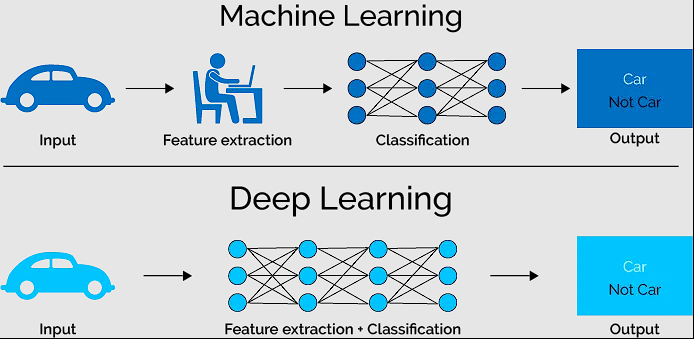
\includegraphics[scale=.75]{figures/traditional_vs_deeplearning.png}}
    \caption{Side-by-side comparison of traditional machine learning (with manual feature extraction) and deep learning (automatic feature extraction)~\cite{mahapatra2018deep}.}
    \label{fig:trad_and_deep}
    \end{figure}


The advancement of automation has only bolstered Deep Learning's relevance. 
In diverse applications, from robotic processes to customer service automation 
and even the intricate algorithms guiding self-driving vehicles, deep learning 
acts as the backbone. It provides these systems the tools to comprehend their 
environment and subsequently make informed decisions. This integration ensures 
not only unprecedented speed and efficiency but also a level of reliability and 
precision often surpassing human-driven processes.\\

Another frontier that deep learning is significantly influencing is Industry 4.0. 
This term, synonymous with the Fourth Industrial Revolution, marks the ongoing 
transformation characterized by heightened automation and data exchange in manufacturing 
technologies. It encompasses innovations like cyber-physical systems, the ever-expanding 
Internet of Things (IoT), cloud and cognitive computing. Within this ecosystem, deep learning 
emerges as a game-changer. Imagine a manufacturing setup where sensors constantly relay data 
from equipment. Deep learning models, acting on this data, can preemptively detect when a 
component might fail, ensuring timely maintenance, drastically reducing downtime, and 
invariably enhancing production efficiency.\\

To encapsulate, the significance of deep learning in our evolving technological 
landscape is huge. Whether it’s in the seemingly mundane, like fine-tuning song or movie recommendations, or in the deeply impactful, such as diagnosing ailments from medical images or forecasting calamities, deep learning prevails. 
As the world becomes increasingly data-centric, the unparalleled processing and analytical 
capabilities of deep learning models ensure that they remain not just relevant, but 
indispensable. In many ways, deep learning is not merely a trend within artificial 
intelligence; it represents an bold stride towards devising machines that think and 
learn akin to humans, yet operate on scales unfathomable to human cognition.\\

\subsection{Deep Learning Essentials}

Deep learning has become a driving force behind various state-of-the-art applications in numerous domains. The following core concepts elucidate the foundational pillars of deep learning, providing insights into its inner workings and methodologies.

\subsubsection*{Neural Networks}

\begin{figure}[htbp]
    \centering
    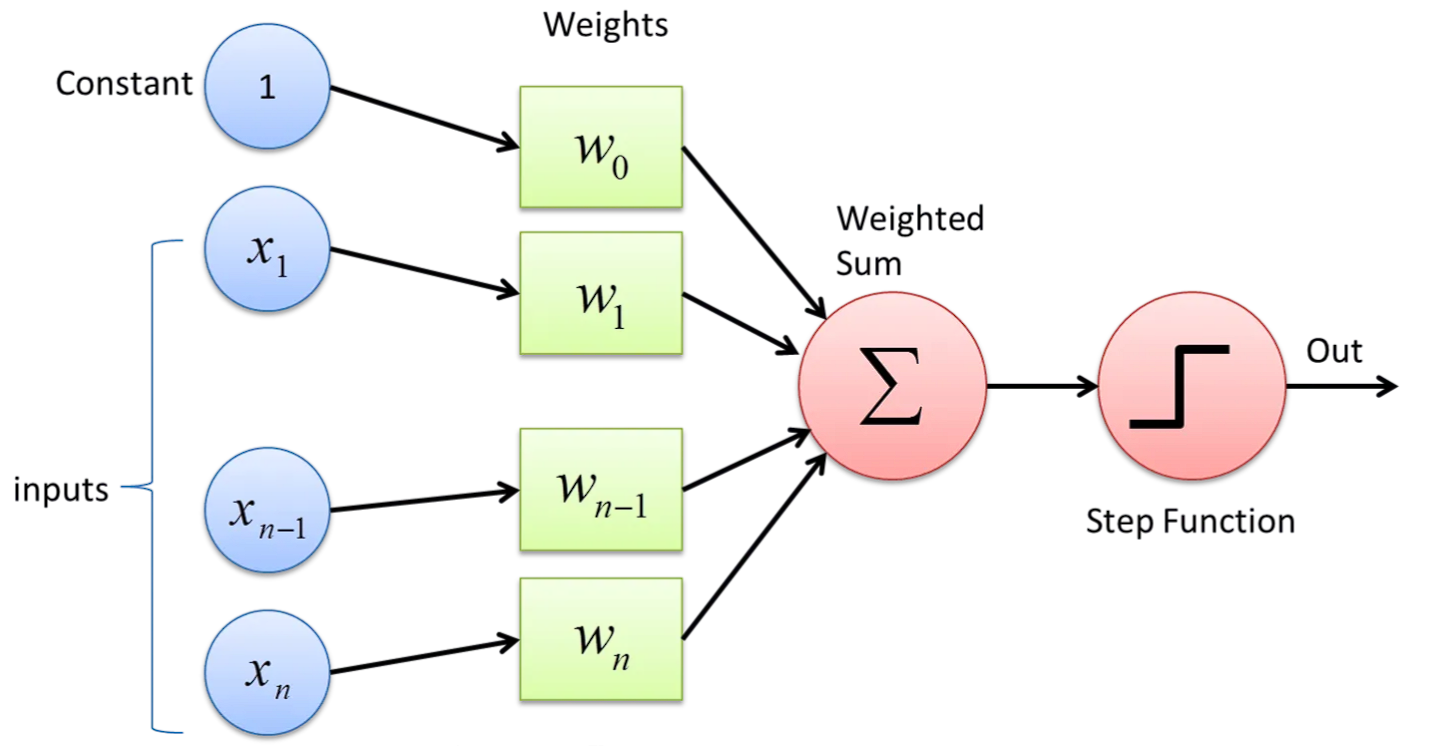
\includegraphics[width=\textwidth]{figures/perceptron.png}
    \caption{A perceptron, the basic building block of neural networks.~\cite{sharma2017perceptron} }
    \label{fig:perceptron}
\end{figure}

Neural networks are the foundational building blocks of deep learning. They are inspired by the structure and functioning of the human brain's interconnected neurons. The concept of neural networks has gained immense popularity due to their ability to learn complex patterns and representations from data. By simulating the interconnectedness of neurons, neural networks can capture hierarchical features in data, making them suitable for tasks such as image recognition, natural language processing, and more. The layers in a neural network (input, hidden, and output) allow for the extraction of progressively abstract features from the input data, enabling the model to make accurate predictions.

The fundamental unit of a neural network is a perceptron, as illustrated in Figure~\ref{fig:perceptron}. Proposed by Frank Rosenblatt in 1957, the perceptron marked the inception of automated feature extraction, a cornerstone of deep learning's superiority over traditional machine learning. Rosenblatt's seminal work, titled "The Perceptron, a Perceiving and Recognizing Automaton," showcased the initial steps towards automating the identification of essential features in data, a concept that is deeply ingrained in today's deep learning models~\cite{rosenblatt1957perceptron}.

\subsubsection*{General Structure of an Artificial Neural Network}
An Artificial Neural Network (ANN) comprises three main types of layers: the input layer, hidden layers, and the output layer. 

\begin{itemize}
    \item \textbf{Input Layer:} The input layer consists of neurons that receive the input data and pass it on to the network. Each neuron in this layer corresponds to one feature in the input data.
    \item \textbf{Hidden Layers:} The hidden layers contain neurons that perform computations and transfer information from the input layer to the output layer. The complexity of the neural network increases with the number of hidden layers and the number of neurons in each hidden layer.
    \item \textbf{Output Layer:} The output layer contains neurons that provide the final output of the network. The type of problem (e.g., binary classification, multi-class classification, regression) dictates the number of neurons in the output layer and the activation function used.
\end{itemize}

Each neuron in a layer is connected to all neurons in the previous and subsequent layers, and these connections have associated weights. The weights (\(w\)) and biases (\(b\)) are parameters that are learned from the data during training. They are crucial for the network's ability to make accurate predictions. The weights control the strength of the connection between two neurons, and the biases allow the neurons to have some flexibility in activation. During the training process, the weights and biases are adjusted to minimize the difference between the predicted output and the actual target values, making the model more accurate over time. This process is driven by the backpropagation algorithm, which computes gradients of the loss function with respect to the weights and biases. The activation function within each neuron introduces non-linearity, enabling the network to learn complex patterns. The loss function quantifies the discrepancy between the network's predictions and the actual data, guiding the optimizer in adjusting the weights and biases to minimize this loss.

The output \( y \) of a neuron is given by the equation:
\[
y = f(\mathbf{w} \cdot \mathbf{x} + b)
\]
where \( \mathbf{w} \) is the vector of weights, \( \mathbf{x} \) is the vector of inputs, \( b \) is the bias, and \( f \) is the activation function. A graphical illustration of the process within a neuron is depicted in Figure~\ref{fig:neuron_math}, showing the linear combination of weights and inputs, the addition of the bias, and the application of the activation function to produce the output.

\begin{figure}[htbp]
    \centering
    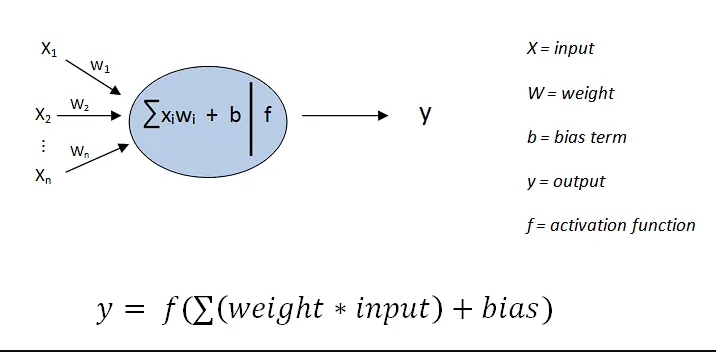
\includegraphics[width=\textwidth]{figures/weights_and_biases.png}
    \caption{Graphical representation of a neuron showing the weights, inputs, bias, and activation function.~\cite{yildirim2020activation}}
    \label{fig:neuron_math}
\end{figure}

\subsubsection*{Activation Functions}

Activation functions introduce non-linearity to the neural network, allowing it to approximate and learn complex relationships in data. Without activation functions, neural networks would only be capable of representing linear transformations, severely limiting their expressive power. ReLU, Sigmoid, and Tanh are commonly used activation functions, each with its unique properties. ReLU addresses the vanishing gradient problem, Sigmoid maps inputs to a sigmoid-shaped range suitable for binary classification, and Tanh is often used in hidden layers to map inputs to a range between -1 and 1. The mathematical expressions for these activation functions and in Figure \ref{fig:activation_functions} a graph of these functions are presented below.

\begin{itemize}
    \item \textbf{ReLU (Rectified Linear Unit):} 
    \[ f(x) = \max(0, x) \]
    
    \item \textbf{Sigmoid:} 
    \[ f(x) = \frac{1}{1 + e^{-x}} \]
    
    \item \textbf{Tanh:} 
    \[ f(x) = \tanh(x) = \frac{2}{1 + e^{-2x}} - 1 \]
\end{itemize}

\begin{figure}[h!]
\centering
\begin{tikzpicture}
\begin{axis}[
  axis lines=center,
  domain=-3:3,
  ymax=1.5,
  ymin=-1.5,
  samples=100,
  legend pos=north west
]
\addplot[blue, thick] {max(0, x)}; 
\addplot[red, thick] {1/(1 + exp(-x))}; 
\addplot[green, thick] {(2/(1 + exp(-2*x))) - 1};
\legend{ReLU, Sigmoid, Tanh}
\end{axis}
\end{tikzpicture}
\caption{Visualization of Activation Functions}
\label{fig:activation_functions}
\end{figure}


\subsubsection*{Loss Functions}

Loss functions quantify the difference between predicted and true values, providing a measure of how well the model is performing. They serve as the basis for optimization, helping the model adjust its parameters to minimize the discrepancy between predictions and ground truth. Different loss functions are used for different tasks; Mean Squared Error (MSE) is well-suited for regression tasks, while Cross-Entropy is commonly used for classification tasks. The choice of the appropriate loss function depends on the nature of the problem the neural network is tackling.

\begin{itemize}
    \item \textbf{Mean Squared Error (MSE)} for regression tasks:
    \[ L(y, \hat{y}) = \frac{1}{n} \sum_{i=1}^{n} (y_i - \hat{y}_i)^2 \]

    MSE is used for regression tasks where we predict continuous values. It's chosen because it penalizes larger errors more, it's differentiable for efficient optimization, and its convex nature aids in finding optimal solutions.
    
    \item \textbf{Cross-Entropy} for classification:
    \[ L(y, \hat{y}) = -\sum_{i} y_i \log(\hat{y}_i) \]

    Cross-Entropy is for classification tasks. It's based on probabilities, making it suitable for class probabilities interpretation. Its logarithmic nature amplifies differences between predicted and true class probabilities, aiding optimization. Also, its gradient doesn't saturate, ensuring continuous learning.

\end{itemize}


% \todo[inline]{Visualization: You can insert specific diagrams or visualizations for Loss Functions}


\subsubsection*{Optimizers}

Optimizers play a crucial role in training neural networks by adjusting the model's parameters to minimize the loss function. Gradient Descent and its variants, such as Stochastic Gradient Descent (SGD), SGD with Momentum, and Adam, are pivotal in this endeavor. These optimizers iteratively modify the model parameters, aiming to find the minima of the loss function, which in turn enhances the model's performance.

\begin{itemize}
    \item \textbf{Gradient Descent (GD):} The algorithm aims to find the minimum of a function \( F \) by iteratively moving in the direction of steepest descent, as defined by the negative of the gradient \( \nabla F \) at the current point \( \mathbf{x}_n \). The update rule is given by 
    \[ \mathbf {x}_{n+1} = \mathbf {x}_n - \gamma_n \nabla F(\mathbf {x}_n),\ n\geq 0 \]
    where \( \gamma_n \) is the learning rate at iteration \( n \).

    \item \textbf{Stochastic Gradient Descent (SGD):} Unlike GD, SGD approximates the gradient using a single training example, which can lead to faster convergence. The update for each parameter \( w \) is 
    \[ w := w - \eta \nabla Q_i(w) \]
    where \( \eta \) is the learning rate.

    \item \textbf{SGD with Momentum:} This variant accelerates SGD by adding a momentum term, which serves to dampen oscillations and speed up convergence. The update rule is:
    \[ v_t = \mu v_{t-1} - \eta \nabla Q_i(w) \]
    \[ w := w + v_t \]
    where \( \mu \) is the momentum term. (See \textit{On the importance of initialization and momentum in deep learning} by Sutskever et al.,~\cite{sutskever2013importance} for more details.).

    \item \textbf{Adam:} The update rule for the parameters \( w \) in Adam is defined as 
    \[ w_{t} = w(t-1) - \alpha \cdot \left( \frac{\hat{m_t}}{\sqrt{\hat{v_t}} + \epsilon} \right), \]
    where \( w_t \) and \( w(t-1) \) are the parameter vectors at time \( t \) and \( t-1 \) respectively, \( \alpha \) is the learning rate, \( \hat{m_t} \) and \( \hat{v_t} \) are bias-corrected estimates of the first and second moment, and \( \epsilon \) is a small constant to prevent division by zero.
\end{itemize}




\subsubsection*{Backpropagation}

Backpropagation is a fundamental algorithm for training neural networks. It is vital because it enables neural networks to learn from data by adjusting their weights and biases. The process involves calculating the gradients of the loss function with respect to each parameter using the chain rule from calculus. These gradients guide the optimization algorithm in adjusting the model's parameters to minimize the prediction error. To visually represent how backpropagation operates within a neural network, we present Figure \ref{fig:backrop} below. Backpropagation is crucial for enabling neural networks to learn complex relationships in data, as it iteratively fine-tunes the model's parameters based on the feedback provided by the gradients.

\begin{figure}[htbp]
    \centerline{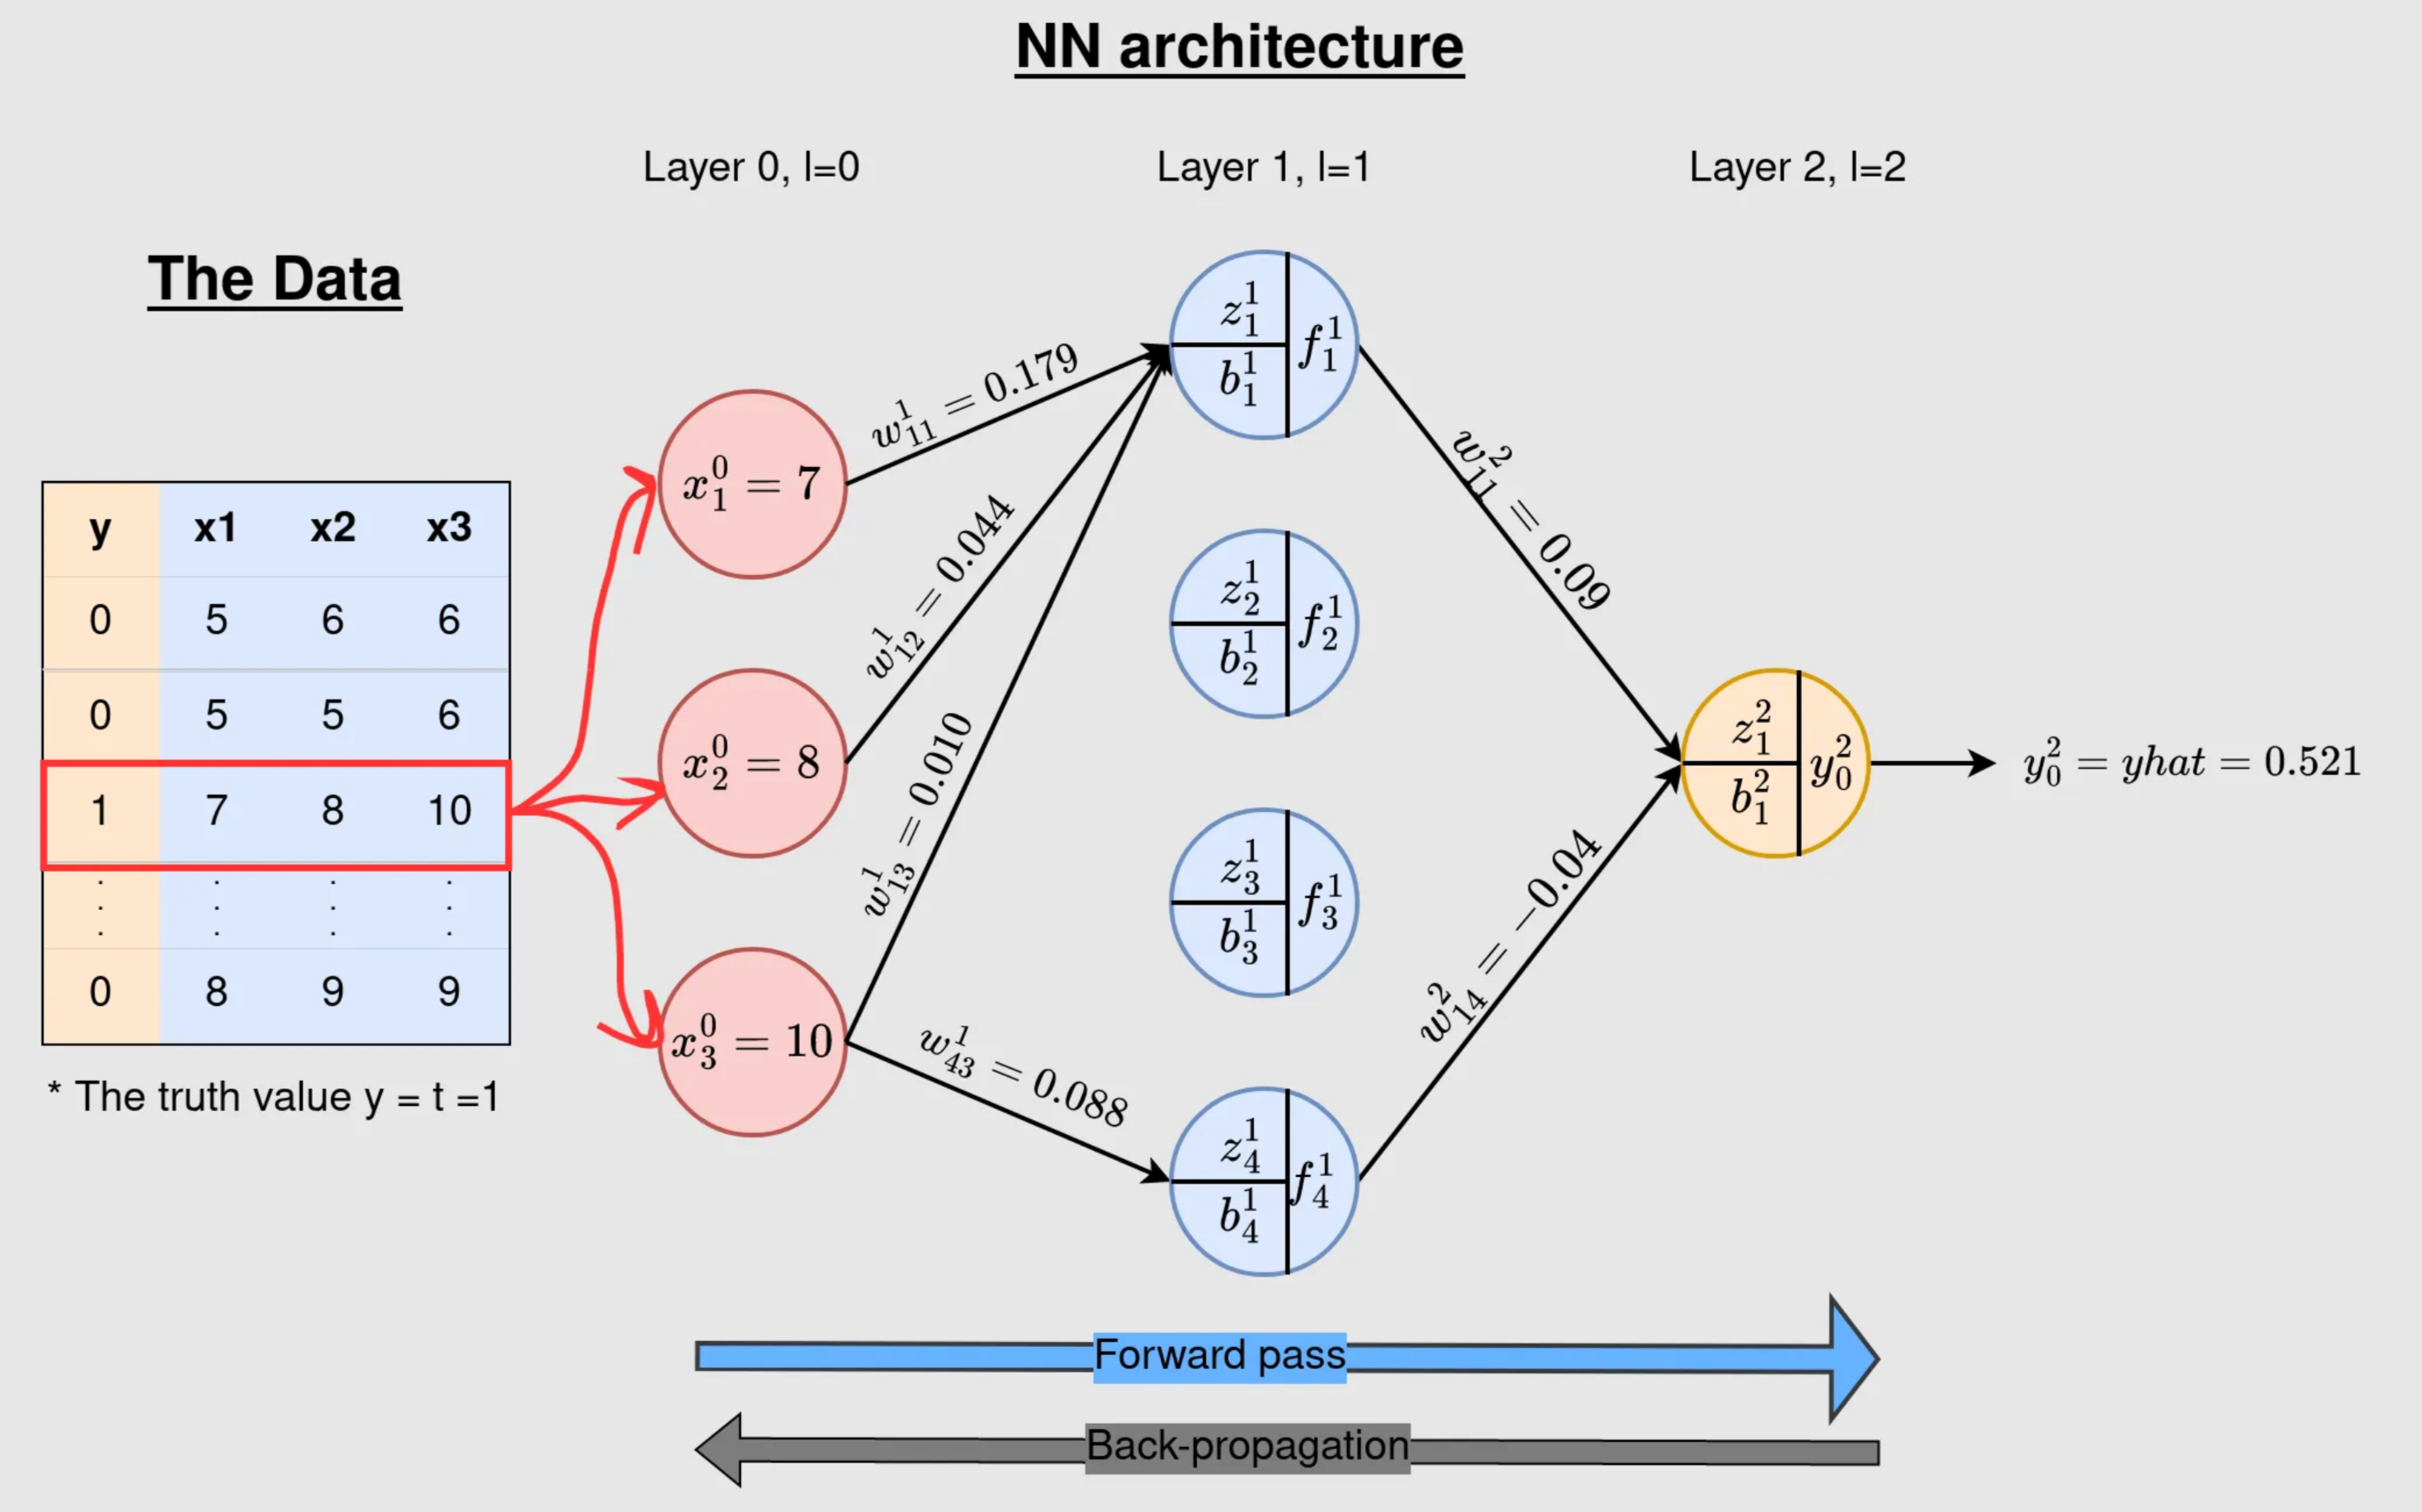
\includegraphics[scale=.29]{figures/backpropagation.png}}
    \caption{Example basic Neural Network Architecture~\cite{koech2022backpropagation} }
    \label{fig:backrop}
    \end{figure}

Following, with reference to Figure \ref{fig:backrop}, we try to explain the simple weight optimization process with backpropagation:\\

\textbf{1. Activation Function (Sigmoid):}
The sigmoid function, \( \sigma(z) \), and its derivative are given by:
\begin{align*}
\sigma(z) &= \frac{1}{1 + e^{-z}} \\
\sigma'(z) &= \sigma(z)(1 - \sigma(z))
\end{align*}

\textbf{2. Loss Function (Cross-Entropy Loss):}
For binary classification tasks, the cross-entropy loss for a predicted output \( y \) and true target \( t \) is:
\[
L(y, t) = -t \log(y) - (1 - t) \log(1 - y)
\]

\textbf{3. Gradient of the Loss:}
The gradient of the cross-entropy loss with respect to the output \( y \) is:
\[
\frac{\partial L}{\partial y} = \frac{y - t}{y(1 - y)}
\]

\textbf{4. Backpropagation:}
For a single-layer neural network, the gradient of the loss \( L \) with respect to the weight \( w \) is:
\begin{align*}
\frac{\partial L}{\partial w} &= \frac{\partial L}{\partial y} \times \frac{\partial y}{\partial z} \times \frac{\partial z}{\partial w} \\
\frac{\partial L}{\partial w} &= \frac{y - t}{y(1 - y)} \times \sigma(z)(1 - \sigma(z)) \times x
\end{align*}
where \( z = w \cdot x + b \). \\

\textbf{5. Weight Update using SGD:}
The weight is updated as:
\[
w_{\text{new}} = w_{\text{old}} - \alpha \times \frac{\partial L}{\partial w}
\]
Where \( \alpha \) is the learning rate.
\subsubsection*{Batch Normalization}

Batch Normalization is a technique that improves the training stability and convergence speed of neural networks. It normalizes the intermediate feature representations within a neural network batch-wise. This process helps mitigate the vanishing and exploding gradient problems, enabling smoother and faster convergence during training. Batch Normalization also acts as a regularizer, reducing the need for other regularization techniques like dropout.
\[ \hat{x} = \frac{x - \mu}{\sqrt{\sigma^2 + \epsilon}} \]
Where \( \mu \) is the mean and \( \sigma^2 \) is the variance.

\subsubsection*{Transfer Learning}

Transfer Learning leverages knowledge gained from one task or dataset to improve performance on another related task or dataset. This approach is incredibly useful when labeled data is scarce for the target task. Pre-trained models, especially those trained on massive datasets like ImageNet, provide valuable initializations for the model's parameters. Fine-tuning a pre-trained model on a specific task allows the model to learn task-specific features while retaining the general knowledge it gained from the pre-training.\\

However, there can be disadvantages such as negative transfer where the pre-training may misguide the learning on the target task, or overfitting if the target task's dataset is too small.
\begin{itemize}
    \item \textbf{Learning Rate:} This is a crucial hyperparameter that determines the step size taken during each iteration while moving towards a minimum in the loss function. A smaller learning rate might take longer to converge, as it involves tiny steps, but a larger one risks overshooting the optimal point. Properly tuning the learning rate ensures that the model learns efficiently without getting stuck or overshooting.
    
    \item \textbf{Batch Size:} It refers to the number of training samples used in one iteration to update a model's weights. A smaller batch size might lead to more frequent updates, making the model converge faster but possibly with less stability. On the other hand, a larger batch size provides a more general estimate of the gradient, but it requires more memory and might slow down the training.
    
    \item \textbf{Network Architecture:} This refers to the design and structure of the neural network, including the number of layers, the number of units in each layer, and the connections between them. The architecture defines the complexity and capacity of the model. Selecting the right architecture is crucial as it can influence the model's ability to capture intricate patterns in the data.
\end{itemize}

Efficiently tuning these hyperparameters is a challenge but doing so can lead to faster convergence and better model generalization. Techniques like grid search, random search, and Bayesian optimization help navigate the high-dimensional space of hyperparameters to find optimal combinations.~\cite{Claesen2015HyperparameterSI}

\subsubsection*{Performance Metrics}

Performance Metrics quantify how well a model is performing on specific tasks. They provide insights into the model's strengths and weaknesses. 

For classification tasks:

\begin{itemize}
    \item \textbf{Precision:} It is the ratio of correctly predicted positive observations to the total predicted positives.
    \[ \text{Precision} = \frac{\text{True Positives}}{\text{True Positives} + \text{False Positives}} \]

    \item \textbf{Recall (Sensitivity):} It is the ratio of correctly predicted positive observations to all the actual positives.
    \[ \text{Recall} = \frac{\text{True Positives}}{\text{True Positives} + \text{False Negatives}} \]

    \item \textbf{F1-Score:} It is the weighted average of Precision and Recall. It tries to find the balance between precision and recall.
    \[ \text{F1-Score} = 2 \times \frac{\text{Precision} \times \text{Recall}}{\text{Precision} + \text{Recall}} \]

    \item \textbf{ROC (Receiver Operating Characteristics) Curve:} The ROC curve is a graphical representation that illustrates the performance of a binary classifier system as its discrimination threshold is varied. It plots the True Positive Rate (TPR) against the False Positive Rate (FPR) at various threshold settings. The curve starts at the origin (0,0) and ends at (1,1). The diagonal line from (0,0) to (1,1) represents a random classifier, and a good classifier aims to stay as far away from this line as possible (towards the top-left corner).

    \item \textbf{AUC (Area Under The Curve):} It measures the entire two-dimensional area underneath the ROC curve (from (0,0) to (1,1)). AUC represents the degree or measure of separability, indicating how much the model distinguishes between the positive and negative classes.
\end{itemize}

For regression tasks, Mean Absolute Error (MAE) and Mean Squared Error (MSE) measure the deviation between predicted and true values, giving a clear picture of the prediction quality.

\begin{itemize}
    \item \textbf{Mean Absolute Error (MAE):}
    \[ \text{MAE} = \frac{1}{n} \sum_{i=1}^{n} |y_i - \hat{y}_i| \]
    Where:
    - \( n \) is the total number of data points or observations.
    - \( y_i \) is the actual value of the \( i^{th} \) observation.
    - \( \hat{y}_i \) is the predicted value of the \( i^{th} \) observation.
    - \( |y_i - \hat{y}_i| \) represents the absolute difference between the actual and predicted value for the \( i^{th} \) observation.

    \item \textbf{Mean Squared Error (MSE):}
    \[ \text{MSE} = \frac{1}{n} \sum_{i=1}^{n} (y_i - \hat{y}_i)^2 \]
    Where:
    - \( (y_i - \hat{y}_i)^2 \) represents the squared difference between the actual and predicted value for the \( i^{th} \) observation.
\end{itemize}
\subsubsection*{Data Augmentation}

Data Augmentation is essential for training robust and generalized models, particularly in domains like computer vision. By applying domain-specific transformations to the training data, the model becomes less sensitive to variations in the input data, such as rotation, scaling, and cropping. This technique effectively increases the diversity of the training dataset, helping the model learn more representative features and improving its ability to handle real-world data. For a comprehensive understanding and deeper insights into data augmentation techniques, we refer the reader to the seminal work of Shorten et al.~\cite{Shorten2019ASO}.
\subsubsection*{Learning Rate Schedulers}

Learning rate schedulers are algorithms or methods that adjust the learning rate during training based on the number of epochs, iterations, or other criteria. The learning rate is a crucial hyperparameter in training deep neural networks. If set too high, the training might diverge; if set too low, the training might be too slow or get stuck in local minima. By dynamically adjusting the learning rate, schedulers aim to combine the benefits of both high and low learning rates, leading to faster convergence and better generalization.

Here are some popular learning rate schedulers:

\begin{enumerate}
    \item \textbf{Step Decay}: Reduces the learning rate by a factor after a specified number of epochs.
    \item \textbf{Exponential Decay}: Decreases the learning rate at each epoch or iteration exponentially.
    \item \textbf{Cosine Annealing}: Adjusts the learning rate according to a cosine function.
    \item \textbf{ReduceLROnPlateau}: Reduces the learning rate when a metric has stopped improving.
    \item \textbf{Cyclic Learning Rates}: Allows the learning rate to cyclically vary between two bounds.
\end{enumerate}

We focus on the exponential LR and Cosine Annealing LR schedulers.\\

The formula for exponential decay is:

\begin{equation}
\text{lr}(t) = \text{lr}_\text{initial} \times \text{factor}^t
\end{equation}

Where:
\begin{itemize}
    \item $\text{lr}_\text{initial} = 0.001$
    \item $\text{factor} = 0.5$
\end{itemize}

\begin{figure}[h]
    \centering
    \begin{tikzpicture}
    \begin{axis}[
        xlabel=Epochs,
        ylabel=Learning Rate,
        domain=0:32,
        samples=100,
        axis lines=left,
        xmin=0, xmax=32,
        ymin=0, ymax=0.0012,
        xtick={0,4,8,12,16,20,24,28,32},
        ytick={0,0.0002,0.0004,0.0006,0.0008,0.001,0.0012},
        xticklabels={0,4,8,12,16,20,24,28,32},
        yticklabels={0,0.0002,0.0004,0.0006,0.0008,0.001,0.0012},
        tick align=outside,
        axis on top,
        smooth
    ]
    \addplot [mark=none,color=blue] {0.001 * 0.5^(x / 4)};
    \addplot [mark=none,color=red,dashed] coordinates {(0,0.001) (32,0.001)};
    \end{axis}
    \end{tikzpicture}
    \caption{Exponential Learning Rate Schedule (Decay Factor = 0.5)}
\end{figure}

The formula for cosine annealing is:

\begin{equation}
\text{lr}(t) = \text{lr}_\text{min} + \frac{1}{2}(\text{lr}_\text{max} - \text{lr}_\text{min})(1 + \cos(\frac{\pi t}{T}))
\end{equation}

Where:
\begin{itemize}
    \item $\text{lr}_\text{min} = 0$ (usually)
    \item $\text{lr}_\text{max} = 0.001$
    \item $T = 32$
\end{itemize}

In the figure \ref{fig:exponential} we can see the graph cosine annealing learning rate schedule.

\begin{figure}[h!]
    \centering
    \begin{tikzpicture}
    \begin{axis}[
        xlabel=Epochs,
        ylabel=Learning Rate,
        domain=0:32,
        samples=100,
        axis lines=left,
        xmin=0, xmax=32,
        ymin=0, ymax=0.0012,
        xtick={0,4,8,12,16,20,24,28,32},
        ytick={0,0.0002,0.0004,0.0006,0.0008,0.001,0.0012},
        xticklabels={0,4,8,12,16,20,24,28,32},
        yticklabels={0,0.0002,0.0004,0.0006,0.0008,0.001,0.0012},
        tick align=outside,
        axis on top,
        smooth
    ]
    \addplot [mark=none,color=blue] {0.0005 * (1 + cos(180 * x / 32))};
    \addplot [mark=none,color=red,dashed] coordinates {(0,0.0005) (32,0.0005)};
    \end{axis}
    \end{tikzpicture}
    \caption{Cosine Annealing Learning Rate Schedule}
    \label{fig:exponential}
\end{figure}


\subsubsection*{Early Stopping}

Early Stopping is a regularization technique used to prevent overfitting. Training a model for too many epochs can lead to it memorizing the training data rather than generalizing to new data. Early Stopping monitors the validation performance and halts training when the validation loss starts to increase. This prevents the model from deteriorating on unseen data and helps achieve the best trade-off between training performance and generalization.
% You can insert a visualization here showing training vs validation loss and pointing out where early stopping would intervene.


\subsection{Overview of Deep Learning Algorithms}

Deep learning, over the years, has evolved to cater to diverse domains and challenges, leading to the development of several specialized algorithms. These algorithms emerged in response to specific challenges in data representation, computational efficiency, or domain-specific nuances. The diversity in algorithms is primarily a result of attempts to optimize performance across a myriad of tasks.\\

In chronological order, some of the influential deep learning architectures include Feedforward Neural Networks, Convolutional Neural Networks (CNNs), Recurrent Neural Networks (RNNs), Long Short-Term Memory (LSTM) networks, Gated Recurrent Units (GRUs), and Transformer Networks. A brief overview of these algorithms is presented in Table~\ref{tab:deep_learning_overview}.

\begin{table}[h]
\centering
\begin{tabularx}{\linewidth}{|l|X|}
\hline
\textbf{Algorithm} & \textbf{Description} \\
\hline
Feedforward Neural Networks & Early architectures designed for pattern recognition without any cycles or loops. \\
\hline
CNNs & Specialized for processing grid-like data, such as images, using convolutional layers. \\
\hline
RNNs & Designed for sequential data, containing loops to maintain information across sequences. \\
\hline
LSTM & An RNN variant addressing vanishing gradient issues and retaining long-term dependencies. \\
\hline
GRUs & Simplified version of LSTMs, offering similar capabilities with fewer parameters. \\
\hline
Transformer Networks & Attention-based models providing parallel processing capabilities and superior performance in sequence tasks. \\
\hline
\end{tabularx}
\caption{Brief overview of key deep learning algorithms.}
\label{tab:deep_learning_overview}
\end{table}




\subsubsection*{Convolutional Neural Networks}

Convolutional Neural Networks (CNNs), which began to emerge in the 1980s and gained significant popularity by the late 2000s, have brought transformative changes to the field of image processing. One of the pioneering CNNs, the Neocognitron, was introduced by Fukushima in 1980~\cite{fukushima1980neocognitron}. This was followed by LeNet-5, a work by LeCun et al. in 1998~\cite{lecun1995convolutional}. More recent advancements in CNN architectures include models like ConvNeXt~\cite{liu2022convnet} and EfficientNetV2~\cite{tan2021efficientnetv2}.\\ 

Distinct from traditional Feedforward Neural Networks (FNNs)---which process inputs through a series of interconnected layers without loops or cycles---CNNs incorporate convolutional layers. These layers utilize filters to scan an input for specific patterns. This convolutional process significantly reduces the number of parameters in the network, allowing the model to recognize local patterns in data more efficiently.

\begin{figure}[htbp]
    \centering
    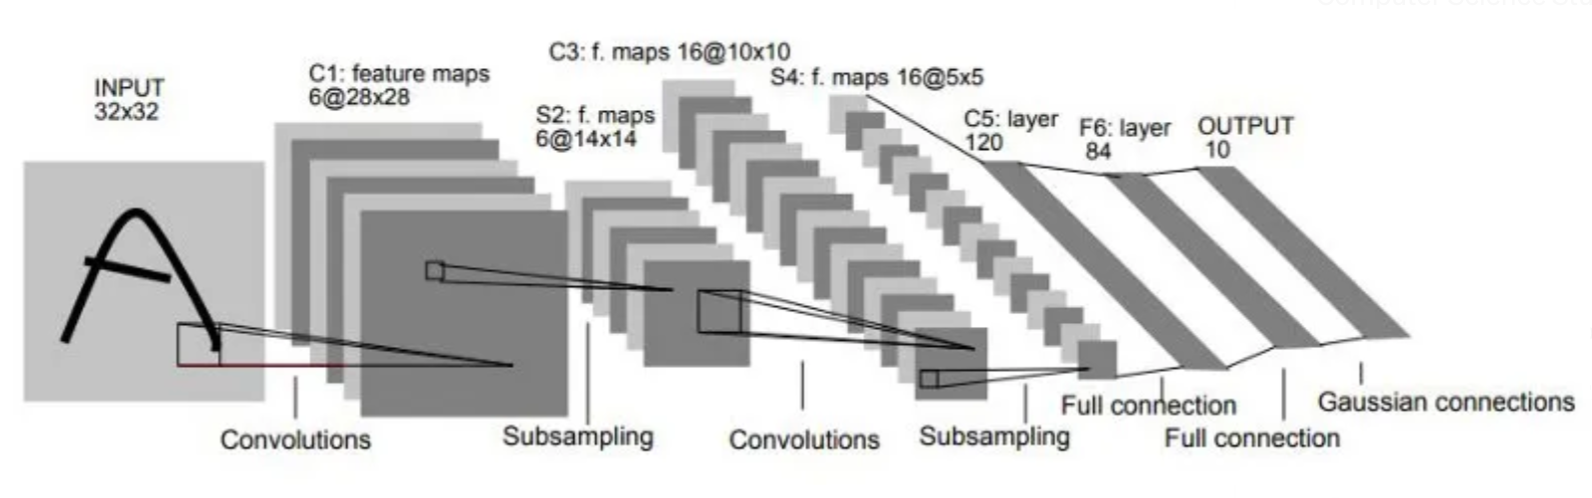
\includegraphics[scale=.5]{figures/lenet.png}
    \caption{Example structure of a CNN~\cite{lecun1995convolutional}. }
    \label{fig:lenet}
\end{figure}

Advantages of CNNs include Parameter Efficiency, which refers to the reduced parameters due to shared weights in convolutional layers; Translation Invariance, highlighting the ability of CNNs to recognize patterns regardless of their position in the input; and Hierarchical Feature Learning, where deep architectures extract layered features, moving from basic to more complex patterns.

% Visualization idea for CNN: A diagram showing how an image is passed through convolutional layers, pooling layers, and fully connected layers.

\subsubsection*{Transformer Networks}
Introduced in the "Attention Is All You Need" paper by Vaswani et al. in 2017~\cite{vaswani2023attention}, Transformers have since dominated various sequence-based tasks, especially in natural language processing. Instead of relying on recurrence, they use self-attention mechanisms to weigh the importance of different parts of the input data.\\

\textbf{Advantages of Transformer Networks:}
\begin{itemize}
    \item \textit{Parallel Processing:} Lack of recurrence allows simultaneous processing of sequence data, leading to speed gains.
    \item \textit{Long-Distance Dependencies:} Captures relationships in data regardless of the distance between elements.
    \item \textit{Scalability:} Easily scales to handle vast datasets and offers state-of-the-art results in many domains.
\end{itemize}

\textbf{Applications:}
\begin{itemize}
    \item Natural Language Processing tasks like translation, summarization, and question-answering.
    \item Time-series forecasting.
    \item Some computer vision tasks leveraging the Vision Transformer architecture.
\end{itemize}

% Visualization idea for Transformer: A diagram showcasing the self-attention mechanism, highlighting how different parts of an input sequence contribute to the output.
\subsection{Applications of Deep Learning}

Deep learning, an advanced subset of machine learning, has fostered a plethora of innovations across numerous domains due to its unparalleled proficiency in handling vast datasets and extracting intricate patterns. The applicability of deep learning transcends sectors, enabling tasks that were once considered the realm of science fiction. For a comprehensive understanding and deeper insights into deep learning and its applications, we refer the reader to the seminal work of Dong et al.~\cite{DONG2021100379}.\\

% \todo[inline]{Visualization: Montage or grid showcasing various applications of deep learning.}
\begin{itemize}
    \item \textbf{Computer Vision:} From basic image classification to advanced tasks like object detection, segmentation, and facial recognition, deep learning, particularly through Convolutional Neural Networks (CNNs), has redefined the boundaries of what machines can perceive. Autonomous vehicles, medical image analysis, and augmented reality are just a few sectors harnessing the power of deep learning-driven computer vision.
    
    \item \textbf{Natural Language Processing (NLP):} Transformer architectures, most notably the BERT and GPT series, have drastically improved machines' ability to understand and generate human language. This has led to improvements in machine translation, sentiment analysis, and chatbots.
    
    \item \textbf{Speech Recognition:} Voice assistants like Siri, Alexa, and Google Assistant are a testament to the prowess of deep learning in understanding and synthesizing human speech, making voice-activated systems more accurate and ubiquitous.
    
    \item \textbf{Healthcare:} From diagnosing diseases with medical imaging to predicting patient trajectories, deep learning is assisting medical professionals by providing tools that can spot symptoms and patterns often too subtle for the human eye.
    
    \item \textbf{Finance:} In the world of finance, algorithms can predict stock market fluctuations, detect fraudulent activities, and automate trading by leveraging deep learning models.
    
    \item \textbf{Entertainment:} Deep learning-driven recommendation systems, such as those employed by Netflix and Spotify, personalize content suggestions, enhancing user experience. Also, Generative Adversarial Networks (GANs) have been used for art creation, game design, and even music generation.
\end{itemize}

While each of these domains has been transformed by the introduction of deep learning, our primary focus will be on \textbf{Computer Vision}. In the subsequent sections, we will delve deep into its intricacies, methodologies, and advancements, painting a comprehensive picture of how machines `see' and `interpret' visual data.
\section{Computer Vision}

Computer Vision (CV) is an interdisciplinary field that seeks to enable machines to interpret and make decisions based on visual data. Drawing inspirations from human vision, pattern recognition, and computational intelligence, CV has emerged as one of the most significant application areas for deep learning. As \textit{Hubel and Wiesel} pointed out in their groundbreaking studies 
on the visual cortex~\cite{Hubel1962ReceptiveFB}, understanding vision is quintessential to understanding intelligence itself.

\begin{figure}[htbp]
    \centering
    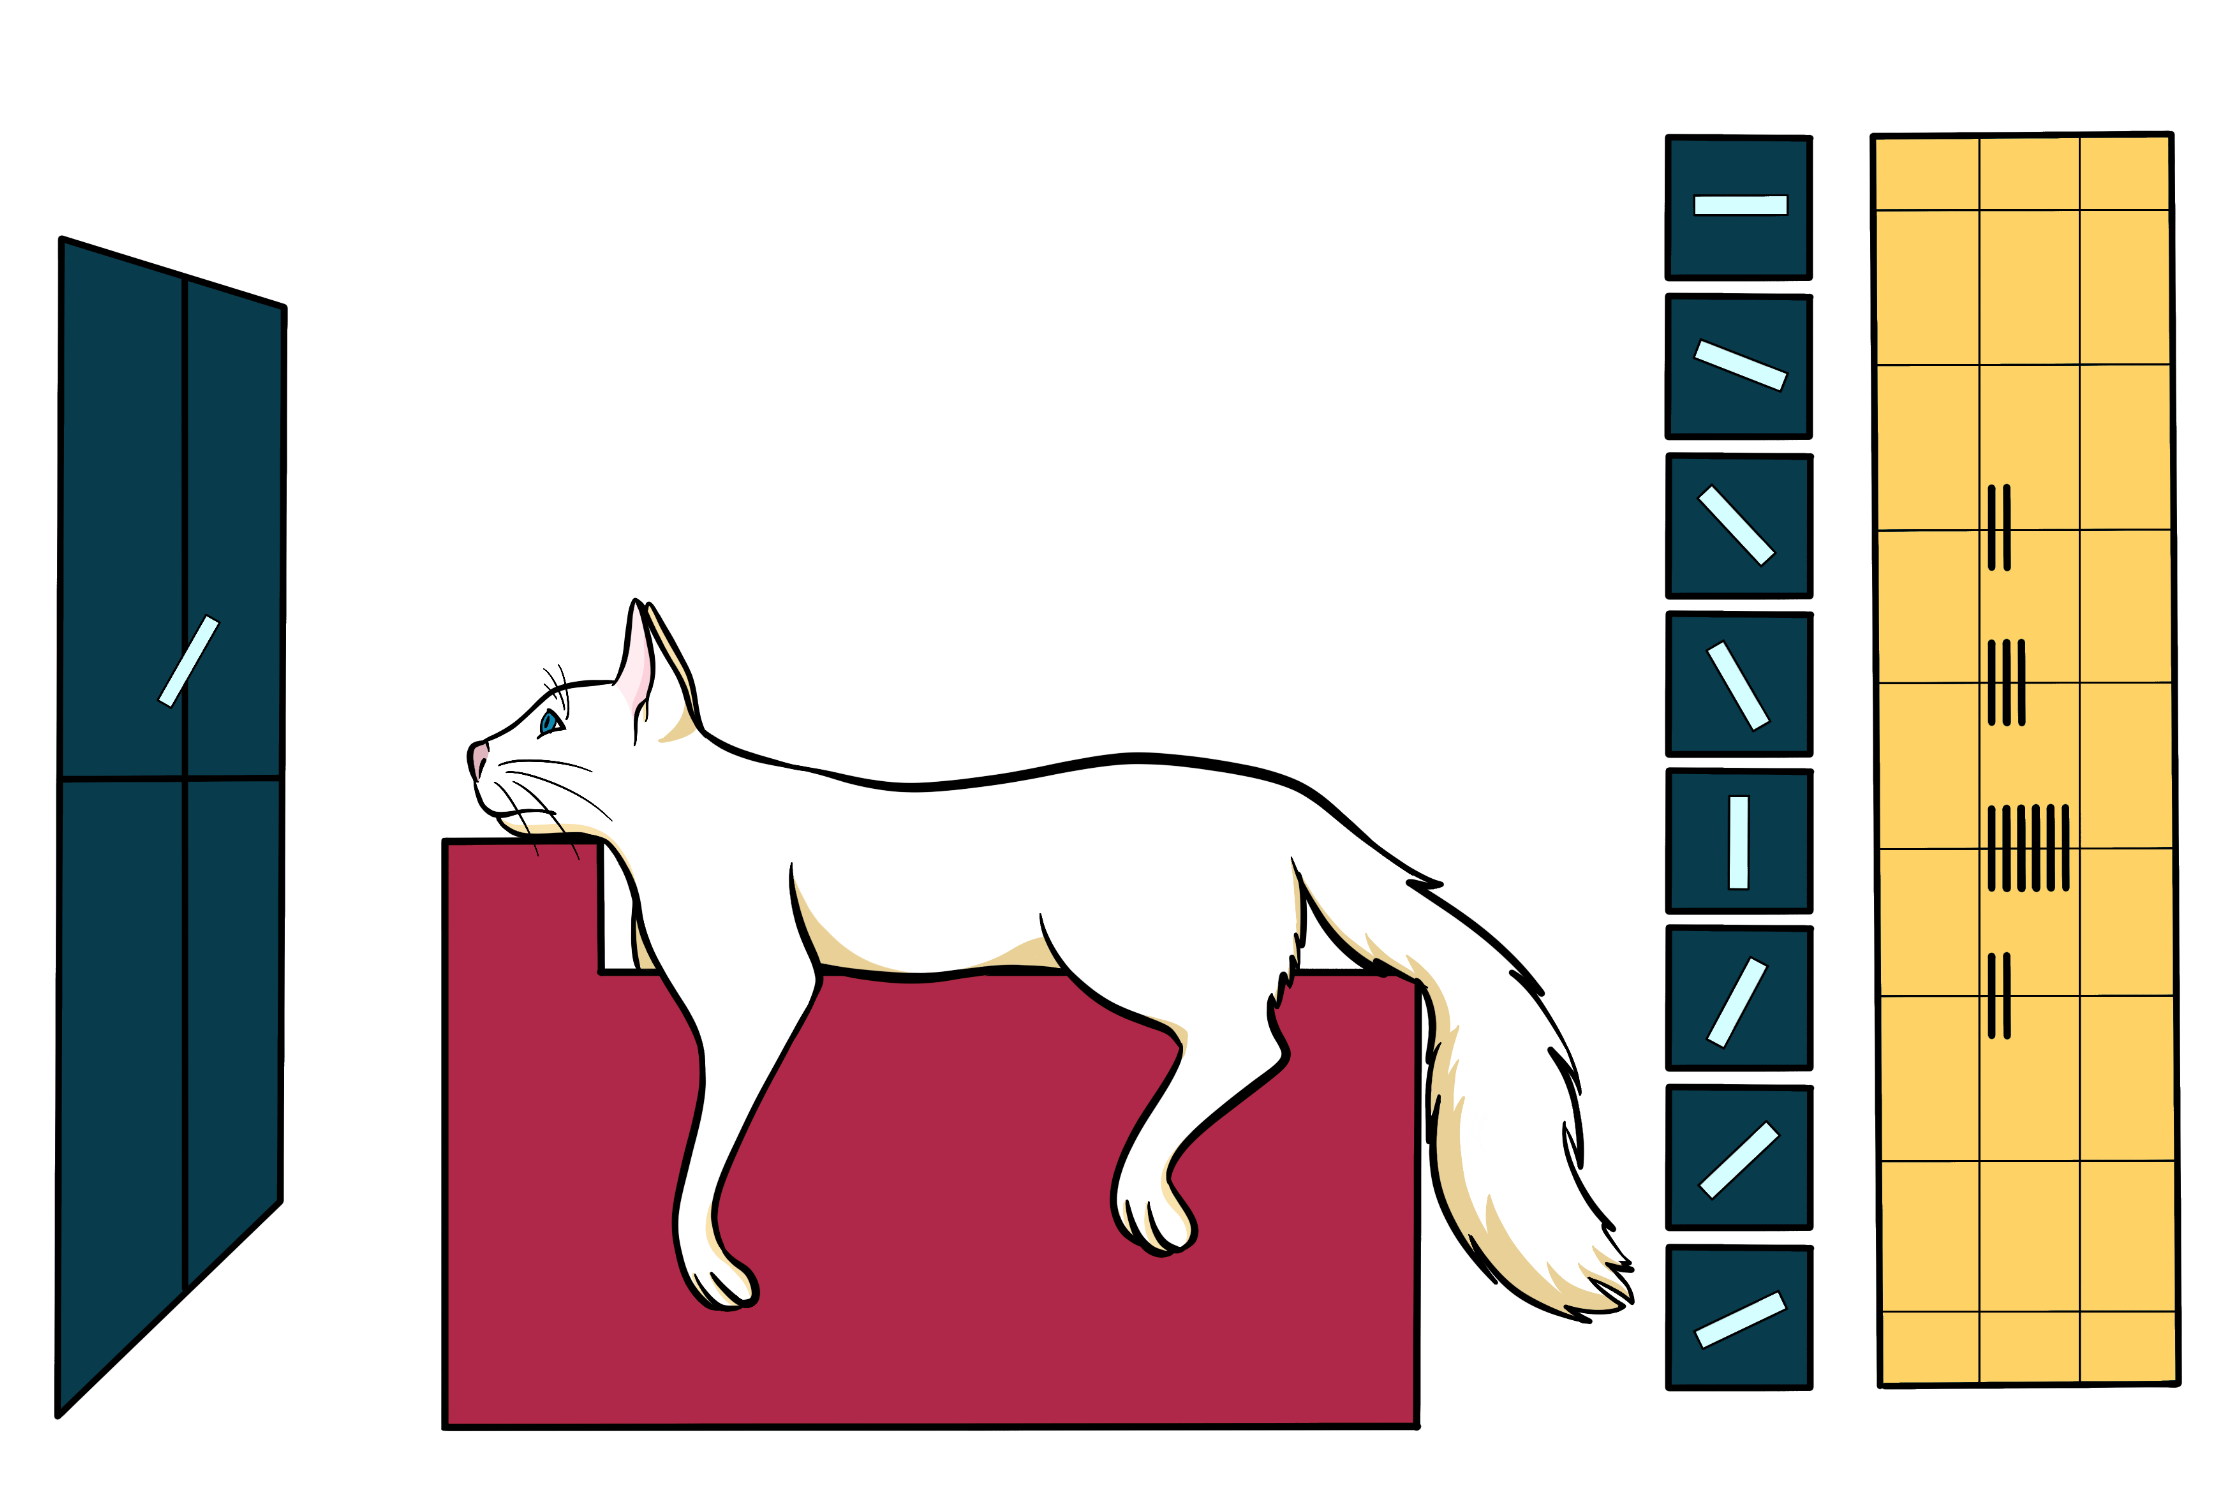
\includegraphics[scale=.3]{figures/cat_experiment.png}
    \caption{Simplified representation of Hubel and Wiesel’s findings on the visual cortex of cats.~\cite{futurelearn2023} }
    \label{fig:lenet}
\end{figure}

\subsection{Image Classification}

At its core, Image Classification is one of the fundamental tasks in computer vision. It involves assigning a predefined label to an input image, usually based on its primary content. For instance, an image containing predominantly a dog would be labeled "dog", irrespective of the breed or its position in the image. In mathematical terms, given an image \(I\), a classifier function \(f\) assigns it a label \(l\) from a set of predetermined labels \(L\):

\[ l = f(I) \]
where \( l \in L \).\\

\begin{figure}[htbp]
    \centering
    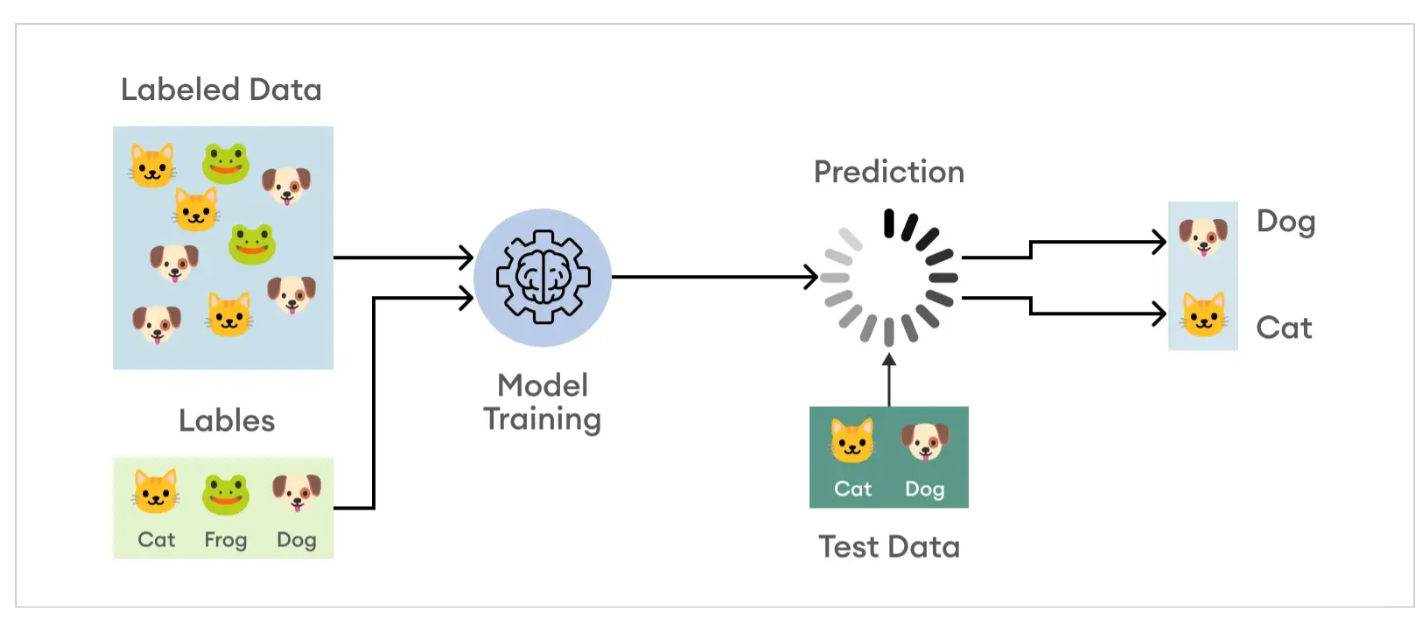
\includegraphics[scale=.5]{figures/image_classification.png}
    \caption{Simple illustration of image classification.~\cite{superannotate2023}}
    \label{fig:lenet}
\end{figure}

\textbf{Applications of Image Classification:}
While the rudimentary idea behind image classification might seem simple, its applications have profound impacts on various sectors:

\begin{itemize}
    \item \textit{Medical Imaging:} Diagnosing diseases by classifying medical images into categories like 'tumor' or 'no tumor'.
    \item \textit{Structural Health Monitoring:} Detecting defects or damages in structures like bridges, buildings, and dams by processing and analyzing images or videos. 
    \item \textit{Agriculture:} Identifying unhealthy plants or predicting the type of crops in satellite imagery.
    \item \textit{Security:} Automated surveillance systems detecting unauthorized or suspicious individuals.
    \item \textit{Retail:} Assisting in automated checkout processes by identifying products.
    \item \textit{Automotive:} In autonomous driving, classifying objects helps vehicles make informed decisions, e.g., distinguishing between pedestrians and lampposts.
    \item \textit{Smart Cities:} Analyzing satellite or drone imagery to plan urban development, detect changes in land use, or estimate population densities.
    \item \textit{Finance:} Document classification to identify types of financial statements or bills.
    \item \textit{Social Media:} Content recommendation based on user's photo uploads or identifying inappropriate content.
\end{itemize}

\textbf{Challenges in Image Classification:}

Despite advances, several challenges remain in image classification:

\begin{itemize}
    \item \textit{Intra-class Variation:} Objects of the same class can appear different under varying lighting, angles, or occlusions.
    \item \textit{Scalability:} As the number of categories increases, distinguishing between them becomes harder.
    \item \textit{Data Imbalance:} Some classes might have fewer training samples than others, leading to biased predictions.
    \item \textit{Transferability:} A model trained on one dataset might not perform well on another due to domain shifts.
\end{itemize}


\section{Reproducibility in Scientific Research}

Reproducibility stands as the foundational pillar upon which the foundation of the scientific method has been built. It functions as a strict check, ensuring that scientific findings remain steady and consistent, regardless of who conducts the experiment.\\

In research, methodological variability often appears as a major challenge. The slightest changes in methodology or experimental procedure can significantly change outcomes. For instance, an experiment conducted at a slightly different temperature or using a slightly different concentration of a reagent can produce different results. As we delve further into research, especially in areas overflowing with big data and high-throughput technologies, the challenges increase. Managing and processing such large amounts of data to ensure reproducibility is a challenging task.\\

Today's research isn't just about test tubes and microscopes; it's closely tied with software. However, as software changes and updates, it introduces another source of inconsistency. An older experiment rerun on a newer software version might yield different results, making reproducibility unclear. This reliance on software, along with the bias towards publishing positive or novel results, means that a significant portion of research, especially those with negative results, remains unpublished.\\

Furthermore, the complexity of the reproducibility issue is highlighted by a survey conducted by Nature, where more than 70\% of the surveyed researchers admitted to having faced challenges in reproducing another scientist's experiments, and over half encountered difficulties reproducing their own experiments. Despite this, most still trust the published literature, showing mixed feelings about reproducibility in the scientific community~\cite{PMID:27225100}.\\

However, the consequences of irreproducible research extend beyond the academic world. The impact of irreproducible research is felt throughout society, leading to wasted resources as other researchers unknowingly follow paths based on incorrect findings. Even more serious, in fields like medicine, the risks are high. Irreproducible research can lead to misguided clinical practices, resulting in wrong treatment methods that can harm patients.\\

\subsection{Irreproducibility in Deep Learning}

Deep within the neural networks of deep learning lies an inherent stochastic nature that brings with it both challenges and opportunities. This randomness, while fundamental to the training processes of deep learning, also introduces a level of unpredictability that can be both a boon and a bane.\\

At the heart of this randomness is the initialization of weights in neural networks. Starting a model's training journey, these weights are often set to random values, acting as the initial step in a long journey towards optimization. Yet, like setting out on a hike from different starting points, these varied initializations can lead the model to different local optima, influencing the final model's performance.\\

Data augmentation, a technique employed to artificially expand training datasets, further introduces variability. By applying transformations like random cropping or rotation, each epoch of training might expose the model to subtle variations of the same data. While this enhances model robustness, it's another source of randomness.\\

Yet, the landscape of randomness in deep learning isn't just about data and weights. Algorithms like Stochastic Gradient Descent (SGD) introduce their own flavor of unpredictability. By using a random subset of data for weight updates, SGD ensures that the model doesn't just memorize data but learns the underlying patterns. However, this very strength is also a source of variability.\\

Beyond these, computational intricacies, such as floating-point precision in digital computations, especially on GPUs, add their own minute variations. Over millions of operations, these tiny discrepancies accumulate, causing significant variability in outcomes.\\

The randomness issue in deep learning is being actively researched. 
Several studies have approached the issue from various angles. 
For instance, Gundersen et al.~\cite{gundersen2022sources}, identified the sources of irreproducibility. 
They found that non-technical sources, such as the initial conditions and the environment of the experiments, affect reproducibility. 
These causes are often related to the mindset and the thinking of the researchers as well as financial constraints. Fig \ref{fig:sources} shows
the non-technical factors that make harder to reproduce any scientific results. These factors indeed valid for deep learning tasks.
Detailed \emph{documentation} with instructions to reproduce to results will help with the reproducibility
and \emph{transparency} on this process would certainly contribute to this cause. Lastly, some \emph{ethics and privacy} regulations could also prevent researchers
to reveal sensitive information, especially in medical domain.
\\

We examine the randomness in this master thesis, which is a technical factor. There are implementation factors and algorithmic factors. These are generally
related with the tooling and the methodology of the experiments. These factors introduce randomness on different level of deep learning process
as a result, variance in the performance occurs. According to Pham et al.~\cite{pham2020problems}, accuracy of the models varies up to \emph{10.8\%}. They conducted a survey as well and
find out that \emph{83.8\%} of the participants unaware of or unsure about implementation level variance. 
Thus, it is reasonable to approach implementation level randomness interrogatively and investigate some standard processes in DL. 
\begin{figure}[htbp]
    \centerline{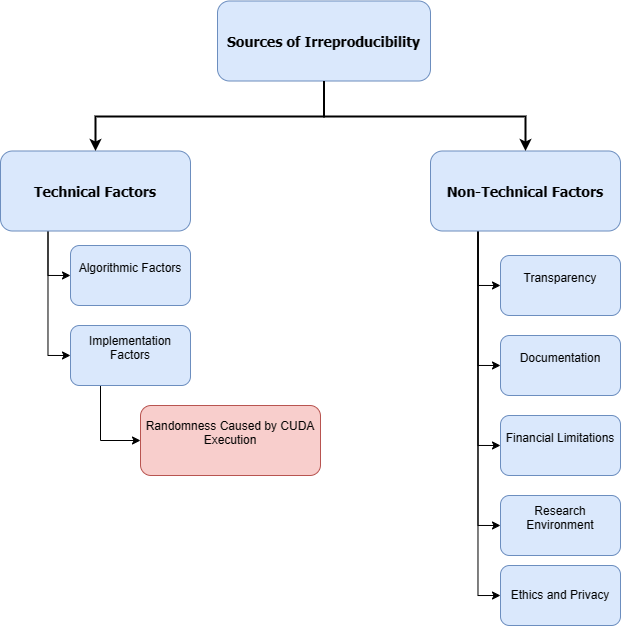
\includegraphics[scale=.5]{figures/Sources.png}}
    \caption{Investigation area of the study.}
    \label{fig:sources}
    \end{figure}
\\
\\
The ripples of this randomness in deep learning extend far and wide. As AI systems become ever more pervasive, from diagnosing diseases to driving cars, unpredictability can pose substantial challenges. Models that yield varying results across runs can complicate evaluations, making direct comparisons challenging. In high-stakes scenarios, like medical diagnoses, this unpredictability can have dire ramifications. Hence, while randomness is an intrinsic aspect of deep learning, understanding, managing, and sometimes mitigating it becomes paramount to harness the true potential of AI.\\
\\

\subsection{Sources of Randomness}
Table \ref{tab:randomness_factors} presents a full list of algorithmic and implementation factors that introduces randomness~\cite{pham2020problems}~\cite{gundersen2022sources}~\cite{zhuang2022randomness}:

\begin{table}[h]
    \centering
    \renewcommand{\arraystretch}{1.5} % Increase row height
    \setlength\tabcolsep{10pt} % Increase space between columns
    \begin{tabular}{|m{0.45\textwidth}|m{0.45\textwidth}|}
    \hline
    \rowcolor{lightgray}
    \textbf{Algorithmic Factors} & \textbf{Implementation Factors} \\
    \hline
    Nondeterministic DL layers that introduce stochasticity & Used framework \\
    \hline
    Random initialization of the weights & Used framework version \\
    \hline
    Hyperparameter optimization & Nondeterministic floating point arithmetic \\
    \hline
    Data augmentation & Parallel execution \\
    \hline
    Data shuffling and ordering & Auto selection of primitive operations \\
    \hline
    Batch ordering & Unpredictability of processing unit \\
    \hline
    \end{tabular}
    \caption{Algorithmic and Implementation Randomness Factors in Deep Learning.}
    \label{tab:randomness_factors}
\end{table}

\subsection{Floating-Point Arithmetics and Parallel Execution}

In the high-performance computing, GPUs have emerged as game-changers. With their vast array of parallel processing units, they have brought unprecedented computational capabilities to the fingertips of developers. NVIDIA's CUDA platform harnesses this power, providing a framework for parallel computing on CUDA-capable GPUs \cite{chetlur2014cudnn}. At the heart of this acceleration lies the intricate dance between floating-point arithmetic and parallel execution.\\

\subsubsection*{Floating-Point Arithmetic: A Double-Edged Sword}

Floating-point arithmetic provides a method to represent and perform operations on real numbers using a finite number of bits. This mathematical framework is fundamental for a multitude of scientific calculations, including those prevalent in deep learning (DL) networks. The primary challenge is that the finite precision of floating-point arithmetic can lead to errors. Although these errors are generally minuscule, their effects can accumulate, notably in iterative algorithms.\\

The IEEE 754 standard delineates the specifics of floating-point arithmetic, fostering consistency across various platforms. This consistency is indispensable, especially given the increasing use of computational methods in scientific research. However, one limitation of the IEEE 754 standard is that, while it prescribes the precision and behavior of singular operations, it doesn't fully govern the sequence of operations or their compound effects. This issue becomes particularly pronounced in parallel computing environments. Here, operations can run concurrently or in an unpredictable sequence, leading to the propagation and magnification of these inherent errors, sometimes resulting in non-deterministic outcomes.

\paragraph{Understanding the Limitations:}

\begin{enumerate}
    \item \textit{Representation Limits:} Not all real numbers can be precisely represented due to the fixed number of bits allocated for floating-point numbers. For instance, the fraction \( \frac{1}{3} \) is a recurring decimal, and its binary representation is similarly recurring. As a result, it's truncated, introducing an error.\\
    
    \item \textit{Rounding Errors:} Numbers that can't be accurately represented lead to rounding errors during operations. For a practical demonstration, in an ideal scenario, \( 0.1 + 0.2 = 0.3 \). Yet, in floating-point arithmetic, this sum might manifest as \( 0.30000000000000004 \) due to inherent representation errors.\\
    
    \item \textit{Error Accumulation:} The cumulative effect of small errors can be significant in iterative processes. Consider an algorithm that repeatedly adds a minuscule value. If the algorithm adds \( 0.0000001 \) a million times, the expected result is \( 0.1 \). However, in floating-point arithmetic, the final sum might diverge slightly from this value.\\
    
    \item \textit{Catastrophic Cancellation:} Subtraction between nearly equivalent floating-point numbers can obliterate significant digits. As an illustrative example, for numbers \( a = 1.0000001 \) and \( b = 1.0000002 \), the difference \( b - a \) should be \( 0.0000001 \). If the precision limits of the system coerce both numbers to round to \( 1.000000 \), the resultant difference becomes zero—a stark contrast to the true value.
\end{enumerate}

In summary, while floating-point arithmetic is a cornerstone of computational methodologies, particularly in DL, its limitations necessitate meticulousness and often compensatory strategies in algorithm design and execution.
\subsubsection*{Parallel Execution in CUDA}

CUDA's parallel execution model divides tasks into threads that are executed across the multiple cores of a GPU. These threads are grouped into blocks, and these blocks are, in turn, organized into grids \cite{chetlur2014cudnn}. This hierarchy allows CUDA to scale computations across different GPU architectures effectively. The figure below illustrates this structure:\\

\begin{figure}[htbp]
\centerline{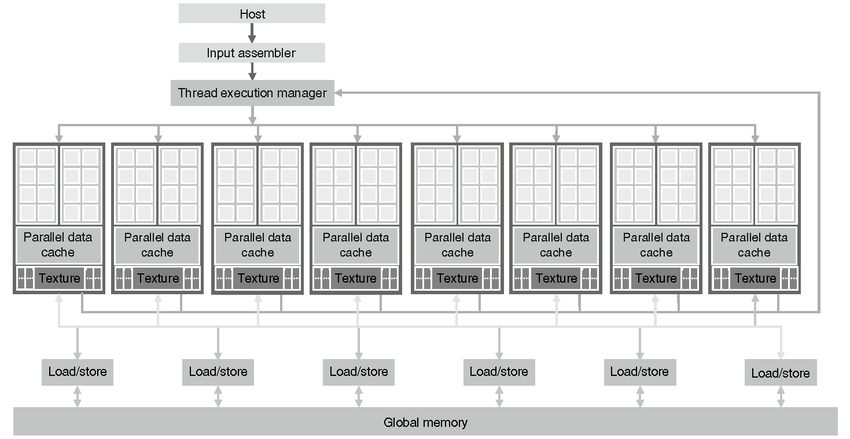
\includegraphics[scale=.5]{figures/cuda.png}}
\caption{CUDA compatible GPU (graphic processor unit) architecture.~\cite{cuda2023} }
\label{fig:cuda}
\end{figure}

However, the inherent nature of parallel execution introduces randomness due to the unpredictable order in which threads are completed. This randomness is exacerbated when combined with the nuances of floating-point arithmetic. Two runs of the same parallel operation can produce slightly different results due to the varying order of execution and the consequent accumulation of floating-point errors.

\subsubsection*{cuDNN: Leveraging CUDA and Introducing Nondeterminism}

cuDNN is a deep neural network GPU-accelerated library that builds upon CUDA \cite{chetlur2014cudnn}. While it greatly boosts the efficiency of DL networks, some of its operations, such as the CUDA convolution benchmarking, are nondeterministic. This nondeterminism stems from both the scheduling of parallel tasks and the intricacies of floating-point precision. Deterministic execution schemes have been proposed to counteract this issue \cite{chou2020deterministic}. However, these schemes can potentially introduce computational overhead.

\subsubsection*{The Trade-Off: Performance vs. Reproducibility}

There's a delicate balance between performance and reproducibility in parallel computing. Deterministic execution schemes increase the reproducibility and credibility of DL networks, making results more trustworthy and comparable across runs. However, they may come at the cost of increased computational time, which could be a significant drawback in time-sensitive applications or large-scale computations. It is, therefore, essential to analyze and understand these trade-offs carefully, tailoring solutions to specific use-cases and experimental setups.\\

In conclusion, the interplay between floating-point arithmetic and parallel execution in CUDA is a complex one. While it offers immense computational power, it also brings forth challenges in reproducibility. As researchers and developers, it's our responsibility to approach these challenges head-on, understanding their roots and implications, and crafting solutions that balance both performance and reproducibility.

\section{Frameworks and Tools}
The success and efficiency of any scientific study often hinge on the careful selection and proficient use of the right computational tools and frameworks. In the scope of this study, several tools and frameworks have been adopted, each with its unique benefits and contributions to the overall experiment. Here, we provide a brief overview of these tools and their significance in the research.

\begin{table}[h]
    \centering
    \renewcommand{\arraystretch}{1.5}
    \begin{tabular}{|l|p{10cm}|}
    \hline
    \textbf{Framework/Tool} & \textbf{PyTorch} \\
    \hline
    \textbf{Publisher} & Facebook's AI Research lab (FAIR) \\
    \hline
    \textbf{Overview} & An open-source deep learning framework with a dynamic computational graph, PyTorch is versatile and suited for research. It allows on-the-fly graph modifications. \\
    \hline
    \textbf{Role in the Experiment} & PyTorch was central to our study, aiding in the design, training, and evaluation of deep learning models. Its adaptability supported quick prototyping and its extensive library eased the deployment of various architectures and methodologies. \\
    \hline
    \end{tabular}
    \caption{Overview of PyTorch}
\end{table}

\begin{table}[h]
    \centering
    \renewcommand{\arraystretch}{1.5}
    \begin{tabular}{|l|p{10cm}|}
    \hline
    \textbf{Framework/Tool} & \textbf{Weights and Biases (W\&B)} \\
    \hline
    \textbf{Publisher} & Weights \& Biases, Inc. \\
    \hline
    \textbf{Overview} & W\&B is crafted to assist researchers in tracking and visualizing ML experiments. It encapsulates features like hyperparameter tuning, model visualization, and performance tracking. \\
    \hline
    \textbf{Role in the Experiment} & W\&B was integral for experiment management, used for logging results, visualizing model dynamics, and comparing architectures and hyperparameters. \\
    \hline
    \end{tabular}
    \caption{Overview of Weights and Biases}
\end{table}

\begin{table}[h]
    \centering
    \renewcommand{\arraystretch}{1.5}
    \begin{tabular}{|l|p{10cm}|}
    \hline
    \textbf{Framework/Tool} & \textbf{SLURM} \\
    \hline
    \textbf{Publisher} & SchedMD \\
    \hline
    \textbf{Overview} & SLURM is an open-source job scheduler, pivotal for resource allocation in multi-user clusters. It's a mainstay in high-performance computing due to its scalability. \\
    \hline
    \textbf{Role in the Experiment} & Given the computational demands of deep learning, SLURM managed our job submissions. It optimized resource allocation, enabling parallel experiment execution without contention. \\
    \hline
    \end{tabular}
    \caption{Overview of SLURM}
\end{table}

The synergy of these tools and frameworks enabled a seamless, efficient, and insightful experimental process. PyTorch offered the foundational deep learning capabilities; Weights and Biases ensured that experiments were tracked, visualized, and optimized; and SLURM managed the computational resources effectively. Together, they ensured that the research was conducted in a structured, efficient, and reproducible manner.
 
\section{Mathematical Evaluation}

In the thesis, several mathematical tools and methods are used to evaluate the results. In this section, we explain these tools and methods.

\subsection*{Standard Variance}
Standard Variance, denoted as \( \sigma^2 \), is calculated using the formula:
\[ \sigma^2 = \frac{1}{n-1} \sum_{i=1}^n (x_i - \bar{x})^2 \]
where:
\begin{itemize}
    \item \( n \) is the number of observations,
    \item \( x_i \) is each individual observation,
    \item \( \bar{x} \) is the mean of all observations.
\end{itemize}
Standard Variance is crucial in machine learning and statistics to understand the dispersion and to normalize the data. It's also vital for gauging the accuracy and the reproducibility of models by analyzing the variance in predictions.

\subsection*{Cosine Similarity}
Cosine Similarity is a metric used to measure how similar two vectors are, regardless of their size. The formula for cosine similarity \( S_C \) between two vectors \( A \) and \( B \) is given as:
\[ S_C(A,B) = \frac{{\mathbf{A} \cdot \mathbf{B}}}{{\|\mathbf{A}\|\|\mathbf{B}\|}} = \frac{{\sum_{i=1}^{n}{A_iB_i}}}{{\sqrt{\sum_{i=1}^{n}{A_i^2}}\sqrt{\sum_{i=1}^{n}{B_i^2}}}} \]
where \( n \) is the dimension of the vectors.
Cosine similarity is extensively used in machine learning for understanding the similarity between vectors or entities, which is fundamental in algorithms like nearest neighbors, clustering, and also in recommendation systems.

\subsection*{T-Test with Population Mean}
The One Sample T-Test is a statistical method used to determine whether the mean of a single sample is significantly different from a known or hypothesized population mean. The formula for the one-sample t-test is given by:
\[ t = \frac{( \bar{x} – \mu)}{(s / \sqrt{n})} \]
where:
\begin{itemize}
    \item \( \bar{x} \) is the sample mean,
    \item \( \mu \) is the theoretical population mean,
    \item \( s \) is the sample standard deviation,
    \item \( n \) is the sample size.
\end{itemize}
The population mean can also be estimated as:
\[ \text{Population mean} = \text{Sample mean} + T \times (\text{Standard error of the mean}) \]

\subsection*{Kruskal-Wallis Test}
The Kruskal-Wallis test is a non-parametric method for testing whether samples originate from the same distribution. It is used for comparing more than two samples that are independent, or not related. The formula for the Kruskal-Wallis test is:
\[ H = \left(N-1\right)\frac{\sum_{i=1}^g n_i(\bar{r}_{i\cdot} - \bar{r})^2}{\sum_{i=1}^g\sum_{j=1}^{n_i}(r_{ij} - \bar{r})^2} \]
where:
\begin{itemize}
    \item \( N \) is the total number of observations across all groups,
    \item \( g \) is the number of groups,
    \item \( n_{i} \) is the number of observations in group \( i \),
    \item \( \bar{r}_{i\cdot} \) is the average rank of group \( i \),
    \item \( \bar{r} \) is the average rank of all the data,
    \item \( r_{ij} \) is the rank of observation \( j \) in group \( i \).
\end{itemize}

\subsection*{ANOVA Test}
Analysis of Variance (ANOVA) is a statistical method used to test differences between two or more means. It divides the variance in a dataset into component parts associated with different sources of variation. In its simplest form (One-Way ANOVA), it can be used to compare the means of three or more independent groups. ANOVA partitions the total sum of squares into components related to the effects used in the model, as expressed in:
\[ SS_{\text{Total}}=SS_{\text{Error}}+SS_{\text{Treatments}} \]
The F-test statistic in ANOVA is calculated as:
\[ F = \frac{MS_{\text{Treatments}}}{MS_{\text{Error}}} = \frac{SS_{\text{Treatments}}/(I-1)}{SS_{\text{Error}}/(n_{T}-I)} \]
where:
\begin{itemize}
    \item \( MS \) is the mean square,
    \item \( I \) is the number of treatments,
    \item \( n_T \) is the total number of cases.
\end{itemize}


\chapter{Literature Review}
\label{chapter:03_literature_review}

This empirical study examines reproducibility and randomness in the AI field. In our review of existing literature, we found limited work that allows for a direct comparison with our results. Nevertheless, a number of relevant studies have addressed aspects of these topics, offering insights and methodologies that are pertinent to our investigation. Below, we provide a concise overview of these works, setting the stage for our own contributions.\\

Goodman et al.~\cite{goodman:2016ca} defined the term reproducibility that we use in this study.
Raste et al.~\cite{Raste} conducted an empirical study to investigate the impact of Randomness 
in several machine learning algorithms. They concluded that transparency in used methods and
datasets is a crucial part to create reproducible results. Chen et al.~\cite{chenetal} listed the challenges 
to reproduce any result of a deep learning model. They emphasized the importance of the reproducible
DL models. They also introduced their approach and solution to mitigate the challenges.
Furthermore, they supported their approach with case studies and presented guidelines. Scarpadane et al.~\cite{scardapane2017randomness} gave an overview of randomness and how they applied in deep learning research.
Dirnagl et al.~\cite{dirnagl2019rethinking} introduced a different 
perspective on research reproducibility in different research areas.
It can be understood that in the past years,
researchers have been investigating reproducibility and randomness from different perspectives. 
There are guidelines on how to achieve reproducibility. Some studies emphasize the importance
of the problem. Enhancing the transparency, accountability, and trustworthiness of AI models requires a focus on Reproducibility in AI research. In this case, this research area aligns with the principles of explainable artificial intelligence (XAI). For an in-depth discussion on XAI, readers can refer to the paper by Arrieta et al.~\cite{arrieta2019explainable}.
\\
\\
However, reproducibility in the AI research area could also be considered as a separate topic from XAI 
if the goal is to improve the methods and practices of conducting and reporting AI 
experiments.
For example, Pranava et al.~\cite{madhyastha2019model}
stated that deep neural network-based models are sometimes vulnerable to randomness during the training
of the models. They investigated the random-seed-based perturbations and proposed a solution
to mitigate standard deviations of the model performance.
Pham et al.~\cite{pham2020problems} analyzed the variance in deep learning software systems. With the immense amount of GPU time,
they use widely-used datasets and models with core DL libraries to perform experiments. Their core contributions are the variance in performance that can be up to 10.8\% and a survey which results suggested that a high percentage of researchers in the area
are not aware of the variances. 
Another valuable empirical study is made by Summers et al.~\cite{summers2021nondeterminism}. Their core contribution is that the nondeterminism factors
result in similar levels of variability.
Snapp et al.~\cite{snapp2021synthesizing} conducted another empirical study with simple models to analyze the irreproducibility in deep networks.
They found out that even with the simplest model reproducibility can be a challenge.
Shallue et al.~\cite{shallue2018measuring} demonstrated the properties of the batch size number and its relation with out-of-sample error. They found that max useful batch size depends on 
the properties of the model, training algorithm and dataset. 
Fellicious et al.~\cite{fellicious2020effects} investigated the different optimizers and architectures with respect to varying initial weights.
As can be seen, there are numerous empirical studies conducted by researchers in recent years.
Their findings and methods to limit or control randomness will be used in this thesis to test the use cases. 
We plan to use deterministic execution methods from the literature. It is not our goal to propose a new method. 
\\
\\
A notable contribution to the discourse on reproducibility and the role of randomness was made by Zhuang et al.~\cite{zhuang2022randomness}, who established a benchmark setup to delineate the attributes of tooling in managing randomness. They posited a binary stance on nondeterminism, advocating for its comprehensive control, failing which, they argue, any control exerted becomes moot. Their investigation further revealed a differential sensitivity to randomness across various subsets of datasets. Moreover, they highlighted the substantial overhead incurred by deterministic approaches. An in-depth exploration into hardware and CUDA-induced randomness was undertaken, wherein the sources of randomness were categorized and analyzed in groups relative to different architectures. The distinct factors of implementation and algorithm were individually regulated and juxtaposed against varying architectures, providing a nuanced understanding of the interplay between these elements and randomness.
In a parallel vein, Chou et al.~\cite{chou2020deterministic} presented a proposition for deterministic execution on GPU platforms, identifying it as a facilitator of reproducibility. This feature will be harnessed in this study to attain deterministic executions whenever there's a necessity to regulate CUDA-induced randomness. Such deterministic controls are instrumental in isolating and understanding the variations in the outcomes, thereby enhancing the reproducibility and interpretability of the results.
\\
\\
In the medical sector, reproducibility is a significant concern, especially in Machine Learning for Health (MLH). McDermott et al.~\cite{mcdermott2021reproducibility} conducted a study to understand the reproducibility challenges in MLH, proposing a taxonomy and defining the broad goals and challenges surrounding reproducibility in this domain. Likewise, Beam et al.~\cite{beam2020challenges} outlined the specific challenges faced when attempting to reproduce machine learning models in healthcare.
In this thesis, one of the use cases is derived from the medical domain. Although a public dataset is employed for this use case, many tasks in the medical domain are hindered by the lack of publicly available datasets. The accessibility of data is a common issue as, oftentimes, datasets in the medical domain are private due to the sensitive nature of medical data. To investigate such tasks from a reproducibility standpoint, special permissions are required to access the necessary data.
The unavailability of public datasets not only hampers the reproducibility and validation of machine learning models but also inhibits collaborative research efforts within the community.





\chapter{Research Methodology}
\label{chapter:04_research_methodo}
To investigate the issue of irreproducibility empirically, we built an experimental setup and a working pipeline. Consistency across runs should be maintained as much as
possible by using the same settings and established methods for control. By accounting for other sources of randomness,
we aim to isolate and document the impact of CUDA execution-related randomness. 
This will involve analyzing performance variance for patterns and correlations. The credibility of the results will be ensured by the correct isolation of the randomness.
we execute the multiple runs while carefully managing all sources of randomness. 
The exact number of runs is depend on factors such as GPU capabilities and environmental conditions, 
but we anticipated 180 independent runs overall. The reasoning for this number will be explained later in this chapter.

\section{Experiment Design and Objectives}
Our investigation revolves around the question of the influence of CUDA-induced randomness on the reproducibility and robustness of deep learning applications, specifically within the realm of computer vision. We have termed this central investigation as the Main Question (MQ):

\begin{quote}
\textbf{MQ:} \textit{What is the overarching impact of CUDA randomness on the reproducibility and performance of deep learning tasks in computer vision?}
\end{quote}

To dissect this question and gain a more granular understanding, we have broken it down into three specific sub-questions:

\begin{enumerate}
    \item Our first sub-question addresses the performance variation in deep learning tasks when we control for other potential sources of randomness but deliberately allow the inherent randomness from CUDA execution. The aim here is to gauge the degree to which CUDA randomness alone can influence the outcome. To this end, we execute five identical runs in each configurations to record the variance and ensure the reliability of our findings. This is encapsulated in:
    \begin{quote}
    \textbf{SQ1:} \textit{What is the extent of performance variability when controlling for other sources of randomness, while allowing for randomness from CUDA execution to be present?}
    \end{quote}

    \item The second sub-question explores the implications of using deterministic settings within CUDA. While deterministic approaches may provide reproducibility, they might come with their own set of trade-offs. By having deterministic CUDA execution in some configurations, we intend to shed light on any potential performance or computational costs associated with such an approach. This is summarized in:
    \begin{quote}
    \textbf{SQ2:} \textit{What is the cost of using deterministic approaches in CUDA randomness?}
    \end{quote}

    \item Lastly, our third sub-question addresses the practical implications of CUDA randomness in specific real-world domains. By utilizing two domain-specific datasets — one from Civil Engineering and the other from Medicine — we aim to unearth the nuances of how CUDA randomness might differentially affect performance and computation costs in these specialized areas. This practical aspect of our research is framed as:
    \begin{quote}
    \textbf{SQ3:} \textit{How does the randomness in Computer Vision impact the task performance and computation cost for specific applications, such as Civil Engineering and Medicine?}
    \end{quote}
\end{enumerate}

By investigating these sub-questions, we hope to provide a comprehensive answer to our main research query, bridging the gap between theoretical understanding and practical implications of CUDA randomness in computer vision-based deep learning tasks.\\

One main solution to reduce the randomness in deep learning applications is fixing the seeds.
Seeding is a fundamental practice in deep learning that allows the random number generator to produce same random numbers everytime. As mentioned, inherent randomness arises from, for example, initialization of weights, data shuffling, and data augmentation. This randomness can lead to variations in model performance and outcomes, even when the model is trained with the exact same parameters and data. By fixing the seed value, often referred to as "setting the seed", we can ensure up to some point that these random operations produce consistent results every time the model is run. This deterministic behavior is crucial when we wish to reproduce results, compare the efficacy of different models, or ensure consistent behavior across runs. 
For experiments, we think that different seed configurations might show different results and sensitivity
to CUDA-caused randomness. Thus, we have five different seed configurations and these are chosen randomly. \\

The strategy detailed above can be better understood through the experimental structure illustrated in the figure \ref{fig:runs_exp}.\\
      
\begin{figure}[htbp]
    \centerline{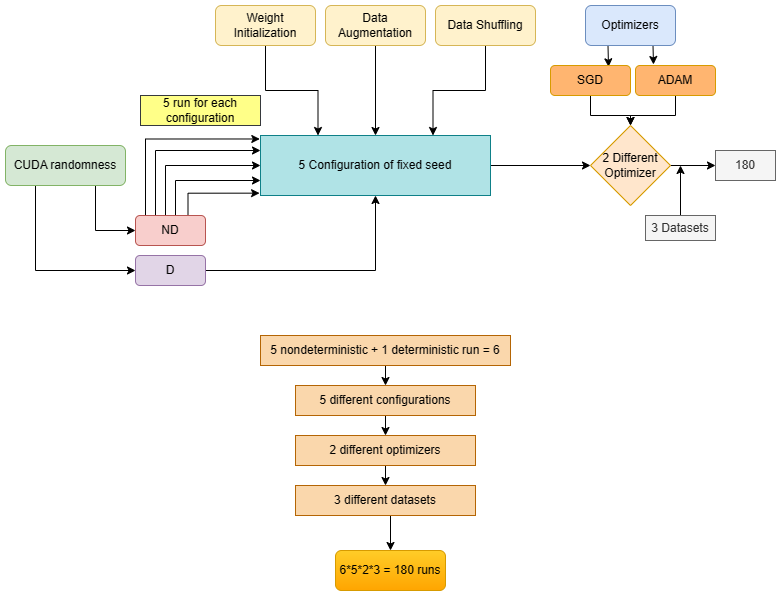
\includegraphics[scale=.5]{figures/runs.png}}
    \caption{Structure of the experimentation}
    \label{fig:runs_exp}
    \end{figure}
 
As can be seen from the figure \ref{fig:runs_exp}, there are \emph{two} options available for randomness settings in CUDA: nondeterministic and deterministic.
There are \emph{five} separate runs using fixed seed configurations
with nondeterministic CUDA settings while controlling all other sources of randomness. That means in the experiments,
framework, used libraries and versions, hardware and other environmental factors will be kept the same.
Additionally, we have \emph{one} run using deterministic CUDA settings.
Ultimetaly, We use \emph{two} commonly used optimizers to find out the optimizer influence and conduct the tests on \emph{three} different datasets,
resulting in a total of \emph{6*5*2*3 = 180}  runs.

\section{Datasets}

In this work, we use only publicly available sources. As a start, CIFAR-10~\cite{krizhevsky2009learning} dataset is used. Experiments on CIFAR-10 will 
provide neutral analysis that would represent the image classification tasks generally and help build the experimentation setup. Additionally,
two different datasets from two different domains will be taken into account. Investigating these two use cases will unlock the 
opportunity to answer the fourth question. 
We use SDNET2018~\cite{maguire2018sdnet2018} as the use case from Civil Engineering. There are several papers that for comparisons and validations. One example is the
work of Dorafshan et al.~\cite{dorafshan2018sdnet2018}.
The researchers showcased their crack detection algorithm's performance by conducting a series of tests using the aforementioned dataset.
The algorithm was developed based on the AlexNet Deep Convolutional Neural Network (DCNN) architecture~\cite{krizhevsky2017imagenet}, which enabled it to achieve accurate results. The dataset is publicly available and usable. 
In the Medical domain, the well-known breast cancer dataset CBIS-DDSM~\cite{spanhol2015dataset} is used.  
The choises of the datasets are made based on some criterias such as ease of applicability, availability, ease of implementation and the number of papers that use the dataset.
\\
\\
\subsection{Overview of the Datasets}

The CIFAR-10 dataset comprises 60,000 32x32 colour images categorized into 10 distinct classes. Each class encapsulates 6,000 images, aggregating to 50,000 training images and 10,000 testing images. The dataset is partitioned into five training sets and a singular testing set. Each training set contains 10,000 images, while the test set encompasses exactly 1,000 randomly chosen images from every category. The training sets exhibit a random order of images, with some sets potentially harboring a higher count of images from a particular category than others. However, cumulatively, the training sets possess an equal distribution with 5,000 images from each category. Table \ref{tab:Cifar-10 labels} delineates the labels within the dataset.\\

\begin{table}[h]
    \centering
    \begin{tabular}{ |c|c| }
        \hline
        Labels & Type \\
        \hline
         0 & Airplane \\
         1 & Automobile \\
         2 & Bird\\
         3 & Cat \\
         4 & Deer \\
         5 & Dog \\
         6 & Frog \\
         7 & Horse \\
         8 & Ship \\
         9 & Truck \\
        \hline
    \end{tabular}
    \caption{Labels in the CIFAR-10 Dataset}
    \label{tab:Cifar-10 labels}
\end{table}

Figure \ref{fig:cifar_10_eda} exhibits a selection of images from each class of the CIFAR-10 dataset, generated using a Python script. The figure elucidates the variability and characteristics inherent in each class, which is instrumental in understanding the complexity of the dataset. It's conspicuous that the dataset encapsulates a diverse range of features and attributes within each class, which underscores the necessity for robust machine learning models capable of discerning nuanced differences and similarities among the images.

\begin{figure}[h]
    \centering
    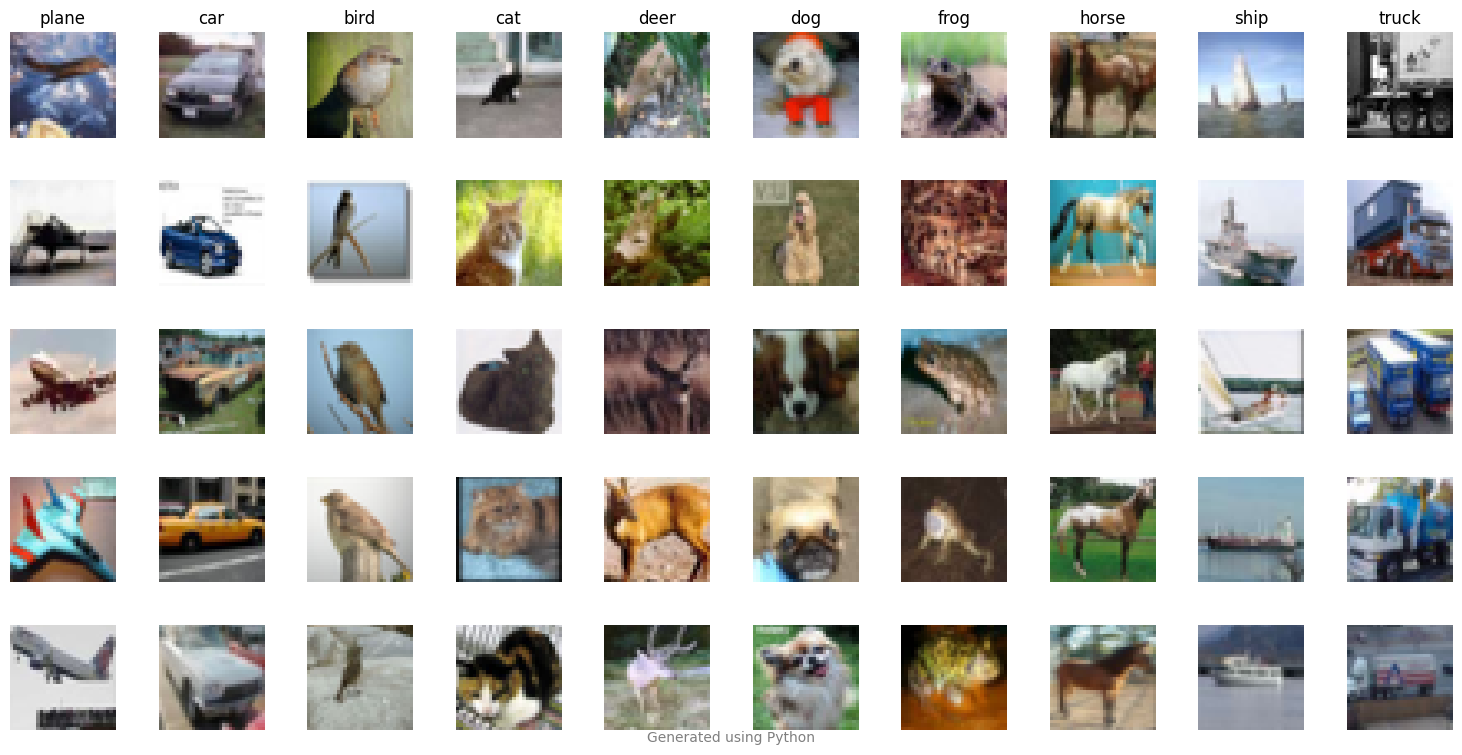
\includegraphics[width=0.8\textwidth]{figures/cifar_10_eda.png}
    \caption{Example images from each class of the CIFAR-10 dataset.}
    \label{fig:cifar_10_eda}
\end{figure}



The SDNET2018 dataset is a comprehensive collection of labeled images specifically designed to aid in the development and evaluation of AI algorithms for detecting cracks in concrete structures. Comprising over 56,000 images, this dataset provides a diverse representation of concrete structures, including walls, pavements, and bridge decks. These images capture both the presence and absence of cracks, with crack widths ranging from a minuscule 0.06mm to a prominent 25mm.\\

What makes SDNET2018 particularly valuable for training machine learning models is its inclusion of images that depict various real-world challenges. These challenges include obstructions such as shadows, surface roughness, scaling, edges, holes, and background debris. Such complexities make the task of automated crack detection more intricate, mirroring the actual challenges faced in real-world scenarios.\\

The ultimate goal of utilizing this dataset is to leverage machine learning and computer vision techniques to pinpoint and localize cracks across diverse structural backgrounds and amidst various obstructions. This is not just a technical challenge but also a matter of public safety. Accurate crack detection is pivotal for assessing the structural health of urban infrastructure, ensuring its longevity, safety, and cost-effective maintenance.\\

A glimpse into the SDNET2018 training set can be seen in Figure \ref{fig:output}, which was generated using a Python script. This figure highlights the varied conditions under which the AI algorithms are expected to operate. The labeled images in the dataset are categorized into two primary labels: "cracked" and "non-cracked". These images display a spectrum of crack appearances and obstructions, emphasizing the real-world intricacies of automated crack detection. Given the variability in crack width, orientation, and the presence of background interferences, there's a pressing need for the creation of robust algorithms. These algorithms should be adept at identifying even the most subtle structural discrepancies in a plethora of cluttered environments.\\

\begin{figure}[h]
    \centering
    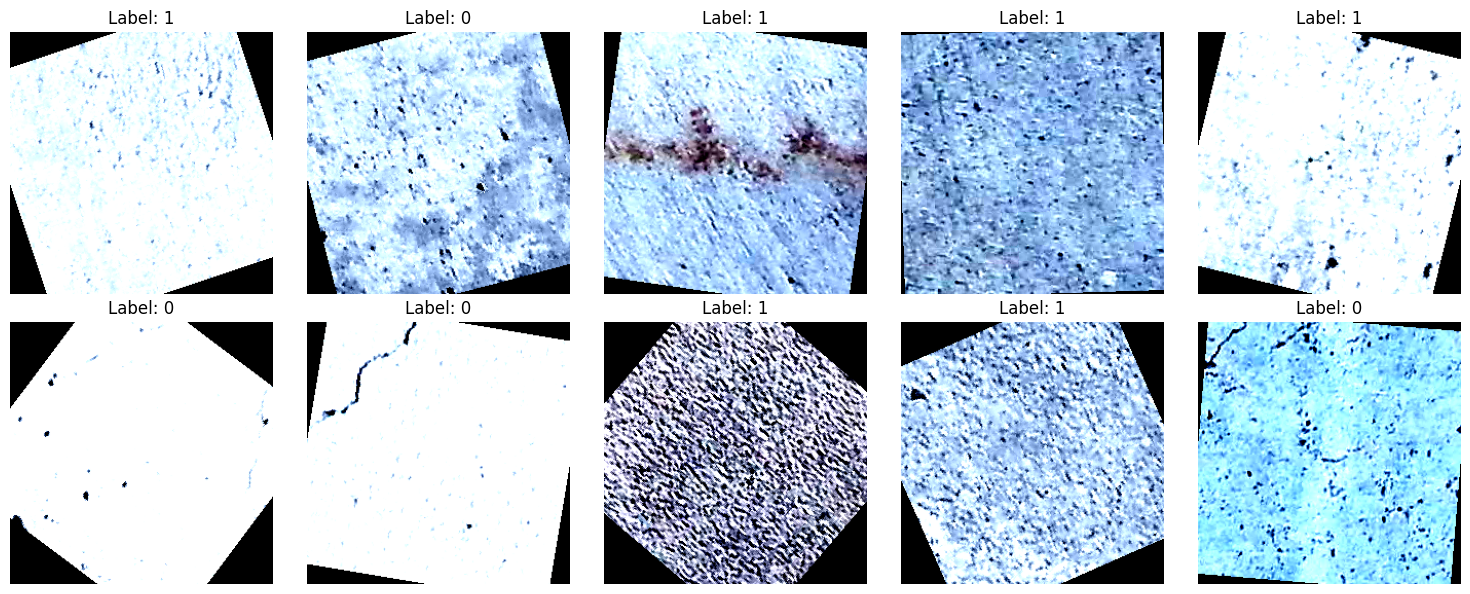
\includegraphics[width=0.8\textwidth]{figures/output.png}
    \caption{Random example images from the SDNET2018 training set with labels.}
    \label{fig:output}
\end{figure}

The CBIS-DDSM (Curated Breast Imaging Subset of DDSM) is a distinguished dataset in the domain of digital mammography research. It originates from the Digital Database for Screening Mammography (DDSM) and is curated to be more accessible for contemporary machine learning and computer vision applications.\\

The core of CBIS-DDSM is composed of mammographic images, encompassing both benign and malignant cases. The images are further categorized based on the type of lesion visible, such as masses or calcifications. The images in CBIS-DDSM have been converted to a more standard format to facilitate modern research, featuring improved lesion annotations and consistent metadata. Each image is accompanied by associated metadata, which may include the patient's age, the type of lesion, its location, and other relevant clinical details.\\

Due to its comprehensive nature and the diversity of cases it presents, the CBIS-DDSM has become an invaluable resource for researchers aiming to develop and validate breast cancer detection algorithms, especially those leveraging machine learning and computer vision.\\

The composition of the CBIS-DDSM dataset is detailed in Table \ref{tab:dataset-composition}, illustrating the distribution of images across different categories. The table segregates the images into benign and malignant cases, and further breaks down the data based on the type of lesions, i.e., masses and calcifications. It is evident from the table that the dataset provides a balanced representation of both benign and malignant cases, which is crucial for training machine learning models to recognize and differentiate between various types of lesions. Moreover, the distinct categorization of lesions into masses and calcifications aids in understanding the diverse nature of mammographic abnormalities present in the dataset, thereby enriching the scope of research in breast cancer detection.\\

% Table showing dataset composition
\begin{table}[h]
\centering
\caption{Composition of CBIS-DDSM Dataset}
\label{tab:dataset-composition}
\begin{tabular}{|l|c|}
\hline
\textbf{Category} & \textbf{Number of Images} \\
\hline
Benign & 1429 \\
Malignant & 1457 \\
Masses & 891 \\
Calcifications & 735 \\
\hline
\end{tabular}
\end{table}

Figure \ref{fig:breast_cancer} displays random example raw images from the CBIS-DDSM dataset, generated using a Python script. The images showcased serve as a stark reminder of the challenges inherent in mammographic image analysis. At a glance, it is difficult, especially for the untrained eye, to ascertain the precise location of cancerous lesions. The subtlety of mammographic abnormalities and the often-ambiguous nature of malignant versus benign indicators render the task of accurate identification and localization exceedingly challenging without substantial domain knowledge and expertise. Moreover, the visual similarity between benign and malignant lesions can further confound accurate classification, underscoring the necessity for sophisticated machine learning and computer vision algorithms capable of teasing apart these nuanced differences to aid in early and accurate breast cancer detection.

\begin{figure}[h]
    \centering
    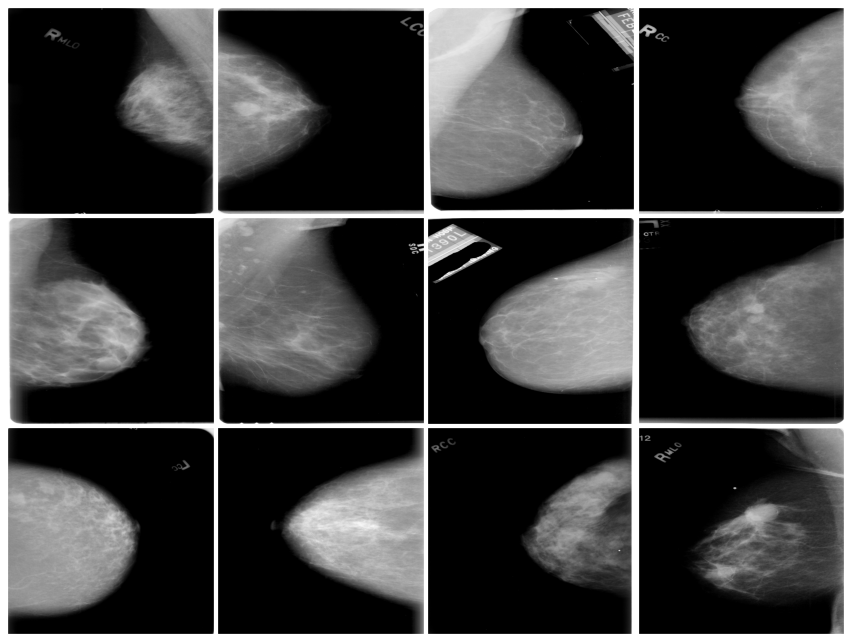
\includegraphics[width=0.8\textwidth]{figures/breast_cancer.png}
    \caption{Random example raw images from the CBIS-DDSM dataset.}
    \label{fig:breast_cancer}
\end{figure}


\section{Model Architectures}

The three tasks at hand involve classifying images and are of particular importance in the fields of civil engineering and medicine,
where they have real-world applications and deal with critical domains. In order to accurately represent real-world scenarios,
there is a strong inclination to achieve high performance on these tasks, which necessitates the use of recent and deep CNN~\cite{lecun1995convolutional} models. 
CNNs extract features from images through convolutional and pooling layers.
Convolutional layers apply filters to small regions of the image, producing feature maps that highlight patterns.
Pooling layers downsample the feature maps to reduce their dimensionality.
This hierarchical feature extraction enables CNNs to learn complex representations of the image, which can be used to classify the image into different categories.
It is important to use CNN models that are commonly used in the scientific community in order to ensure that the results can be validated.
However, hardware and time constraints must also be taken into consideration when selecting models for these tasks, as each run must complete 
in a reasonable amount of time to allow for the timely completion of the experiments. Ultimately, the choice of model will be based on these factors.\\

Three architectures used in this study are PreActResNet~\cite{DBLP:journals/corr/HeZR016}, ResNet~\cite{he2015deep} and MobileNet~\cite{DBLP:journals/corr/HowardZCKWWAA17}. These are used in CIFAR-10, CBIS-DDSM and SDNET datasets, respectively. Below is the short overview of these architectures:\\

\textbf{ResNet (Residual Network)}:
Introduced by Microsoft Research in 2015, ResNet brought the novel concept of "residual blocks" to tackle the vanishing gradient problem in deep networks. This innovation permits the training of considerably deeper networks by introducing shortcut or skip connections that bypass one or more layers. The architecture has several variants including ResNet-18, ResNet-34, ResNet-50, ResNet-101, and ResNet-152, where the numbers indicate the network's depth.\\

\textbf{PreActResNet}:
A variant of ResNet, PreActResNet employs pre-activation within its residual blocks, placing activation functions before weight layers, which has shown improved performance over the original design.\\

\textbf{MobileNet}:
Designed by Google, MobileNet is tailored for efficiency, making it suitable for devices with computational limitations, like mobiles. The architecture's defining feature is its use of depth-wise separable convolutions which substantially reduce the number of parameters, rendering the network lightweight and swift. MobileNet has seen several improvements with versions like MobileNetV1, MobileNetV2, and MobileNetV3, each refining the design to enhance efficiency.\\

The architectures for the three task at hand by chosen their usability, availability and implementation easiness as well as popularity in the community. Another aspect is the limitation of time and hardware. We see that for concrete crack detection we need robust and lightweight architectures as seen in the work of Zhang et al.~\cite{ZHANG2023131941}. Usage of ResNet architectures are so common there are lots of paper that uses these architectures for benchmarks.

\section{Experiment Pipeline}

Our experimental pipeline is based on the the \emph{HPC} infrastructure at IKIM, which is specifically optimized for the computational demands of deep learning. This robust setup ensures that extensive model training and evaluations are conducted seamlessly, harnessing the full potential of modern deep learning methods.\\

Resource allocation and task scheduling are handled by the \emph{SLURM} job scheduler. SLURM's design guarantees that each experiment's computing processes don't overlap with others, ensuring dedicated and consistent computational power. Within this managed environment, our experiments run on Python, primarily utilizing the PyTorch framework. This choice is driven by PyTorch's flexibility in model design, its efficient tensor computations, and its vast library of tools and functions that expedite the deep learning process.\\

Access to \emph{Data} is facilitated via the Network File System (NFS), known for its speed and reliability. During the model training phase, PyTorch dataloaders play a pivotal role by efficiently batching and loading data, optimizing the GPU utilization. To maintain transparency and facilitate analysis, all experimental metrics are logged systematically. Additionally, \emph{Weights \& Biases} (W\&B) provides a platform for real-time visualization and monitoring, giving a clear insight into model performance, convergence rates, and other vital metrics. This structured approach ensures our research remains rigorous, consistent, and informed, as will be shown in the subsequent figure.\\



\begin{figure}[htbp]
    \centerline{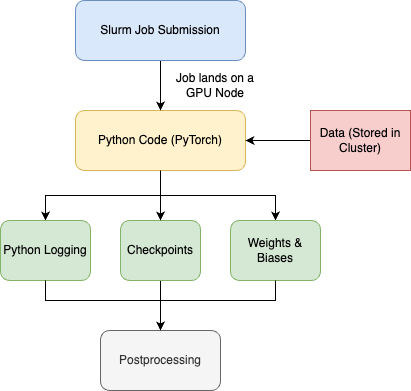
\includegraphics[scale=.5]{figures/Experiments_method.png}}
    \caption{Experiment pipeline}
    \label{fig:exp_pipeline}
\end{figure}


% todo: In-depth explanation of scientific method and how it is applied in our experiments. For example, every data augmentation or anything that is applied to increase the accuracy of the tasks should be mentioned here. Add also how similarities and variances calculated.

\section{Application of Certain Mathematical Methods}

Various mathematical methods have been employed as elucidated in the background chapter, each chosen for specific reasons to align with the objectives of this study. Below, the rationale behind the selection and application of each method is presented.\\

\textbf{Standard Variance:} 
Standard Variance is utilized to assess the dispersion in the outcomes and in the weight matrices, with particular attention to the variance within the last layer of the network. This focus is premised on the pivotal role the last layer plays in classification, embodying the cumulative contributions from all preceding layers. A component-wise standard variance is computed for each checkpoint, yielding a matrix mirroring the original in dimensions but encapsulating the variances in individual weights. The mean of this resultant matrix furnishes the standard variance for a specific configuration at a particular checkpoint. Replicating this process across all checkpoints and configurations facilitates a graphical representation, enabling insightful interpretations of the variance trends.\\

\textbf{Cosine Similarity:} 
Cosine similarity is employed to compare the weights of machine learning models in our study, following the approach of Fort et al. (2020), who utilized this metric for a similar purpose. Cosine similarity is a direct and intuitive measure, providing insight into how the weights diverge, particularly under the influence of CUDA-randomness, during training.\\

The method is applied to examine the similarity among weight matrices. However, a limitation arises as cosine similarity inherently facilitates pairwise comparisons, while our objective is to determine the mutual similarity across five separate runs. To address this, we compute pairwise similarity values for every possible pairing among the five runs, and subsequently average these values to derive a consolidated similarity metric for a given configuration. The procedure is as follows: similarities are computed between the first and second run, first and third run, and so forth, until the final pairing of fourth and fifth run. The mean of these values yields the aggregate similarity for the specific configuration. Further analysis entails extracting the mean, maximum, and minimum values from these computed similarities, which are then visualized to furnish a comprehensive overview of the similarity metrics across various configurations and checkpoints.\\

Referring to the visualizations below, for each distinct configuration, we construct a \(5 \times 5\) matrix showcasing similarity values. The indices within this matrix denote run pairs. By focusing on the lower triangular matrix, we can extract the unique pairs, which are pivotal for subsequent calculations.

\[
\begin{bmatrix}
    (1,1) & (1,2) & (1,3) & (1,4) & (1,5) \\
    (2,1) & (2,2) & (2,3) & (2,4) & (2,5) \\
    (3,1) & (3,2) & (3,3) & (3,4) & (3,5) \\
    (4,1) & (4,2) & (4,3) & (4,4) & (4,5) \\
    (5,1) & (5,2) & (5,3) & (5,4) & (5,5) \\
\end{bmatrix}
\]

The lower triangle, represented as a vector, encapsulates only the unique pairs:

\[
\begin{bmatrix}
    (2,1) 
    (3,1) 
    (3,2) 
    (4,1) 
    (4,2) 
    (4,3) 
    (5,1) 
    (5,2) 
    (5,3) 
    (5,4) 
\end{bmatrix}
\]



\chapter{Experiment Results}
\label{chapter:05_experiment_results}
% !TeX root = ../main.tex

In this section, the reader will be provided with a comprehensive presentation of the results derived from our experiments. These results are juxtaposed not only amongst themselves but also with results from foundational studies, such as the base paper~\cite{zhuang2022randomness}, to highlight differences and commonalities.\\

Throughout this results section, accompanying each set of findings will be explanatory text. This narrative is designed to guide readers, helping them navigate through the figures and understand the salient points. While interpretations and deeper discussions on implications will be reserved for subsequent sections, this portion is instrumental in building a foundational understanding of our experimental outcomes.


\section{Aggregated Results}

In this section, we illuminate the comprehensive performance metrics across diverse configurations and datasets. For contextual clarity, we juxtapose our findings with established results from extant literature. The primary objective of providing these metrics was to offer readers a foundational understanding of the experimental landscape and the inherent complexities involved.\\

It is imperative to underscore that our investigations did not prioritize achieving state-of-the-art outcomes. Instead, our primary objective centers around exploring the underlying randomness inherent in the models. Therefore, our resource allocation primarily emphasized this investigation over optimizing performance benchmarks.\\

For each experiment, we adopt conventional baselines, ensuring minimal modifications in terms of performance enhancement. Our methodologies mainly deviate from these baselines in the realm of experimental design and the integration of reproducibility protocols. A noteworthy adaptation is our incorporation of an additional optimizer into the pipeline. While the baseline configurations predominantly rely on a singular optimizer, we introduce a secondary one, necessitating minimal adjustments in hyperparameter tuning.
\clearpage
Shifting focus to the CIFAR-10 dataset, Table \ref{tab:cifar10_updated} delineates the accuracy scores we achieved across various seeds and optimizers. Deterministic columns shows the mean of the five runs for that spefific configuration. We also present the difference between that mean and non-deterministic run in percentage. Owing to the equitably distributed classes in the CIFAR-10 dataset, accuracy remains the predominant metric within the research community.\\

Upon examination of the results, there's a discernible trend where the SGD optimizer consistently outperforms the ADAM optimizer in terms of accuracy, regardless of the seed. Specifically, the highest accuracy we observe with SGD is approximately 94.81\% with a seed value of 42 in the deterministic setting. In contrast, ADAM's performance peaks around 93.07\% with a seed value of 180698 in the non-deterministic mode.\\

This differential further underscores the nuanced behavior of optimizers and their sensitivities to factors like initialization seeds. Notably, our findings resonate with benchmark data from extant literature~\cite{zhuang2022randomness}, affirming the reliability of our evaluations. It should be emphasized that our approach towards CIFAR-10 predictions strictly followed established methodologies, ensuring no employment of advanced techniques.
\begin{table}[h!]
  \centering
  \caption{Results for CIFAR-10 (Accuracy with Difference from Non-deterministic Mean)}
  \label{tab:cifar10_updated}
  \begin{tabularx}{\textwidth}{XlS[round-mode=places, round-precision=2]S[round-mode=places, round-precision=2]S}
  \toprule
     Seed & Optimizer & {Non-deterministic} & {Deterministic} & {Difference from Mean (\%)} \\
  \midrule
    0 & ADAM & 92.662 & 92.19 & -0.509 \\
       & SGD & 94.804 & 94.96 & 0.164 \\
  \midrule
    180698 & ADAM & 93.068 & 92.22 & -0.910 \\
       & SGD & 94.746 & 94.93 & 0.194 \\
  \midrule
    314 & ADAM & 92.178 & 92.17 & -0.009 \\
       & SGD & 94.814 & 94.71 & -0.110 \\
  \midrule
    3407 & ADAM & 92.568 & 92.72 & 0.164 \\
       & SGD & 94.726 & 94.59 & -0.144 \\
  \midrule
    42 & ADAM & 92.536 & 92.71 & 0.188 \\
       & SGD & 94.756 & 94.81 & 0.057 \\
  \bottomrule
  \end{tabularx}
\end{table}

From the data presented in Table \ref{tab:cifar10_updated}, it is evident that the choice of optimizer plays a important role in the observed outcomes. Previous studies in the literature have posited that SGD tends to outperform ADAM when applied to the CIFAR-10 dataset~\cite{gupta2021adam}. Our empirical findings corroborate this assertion. In experiments it is understood that, the ADAM optimizer demonstrates a protracted convergence trajectory, necessitating an increased number of epochs to approach an optimum. Intriguingly, the global optima identified by ADAM diverges from that ascertained by SGD.
In our analysis, when comparing our findings with the results presented in He et al.~\cite{he2016identity}, which employed a more extensive layer architecture, it is evident that our outcomes are consistent and fall within a similar performance range.\\

    
\begin{table}[h!]
  \centering
  \caption{Results for SDNET (F1-Score with Difference from Non-deterministic Mean)}
  \label{tab:sdnet_updated}
  \begin{tabularx}{\textwidth}{XlSSS}
  \toprule
     Seed & Optimizer & {Non-deterministic} & {Deterministic} & {Difference from Mean (\%)} \\
  \midrule
    0 & ADAM & 0.9328 & 0.9370 & 0.449 \\
       & SGD & 0.9249 & 0.9264 & 0.162 \\
  \midrule
    180698 & ADAM & 0.9345 & 0.9382 & 0.395 \\
       & SGD & 0.9233 & 0.9212 & -0.227 \\
  \midrule
    314 & ADAM & 0.9323 & 0.9314 & -0.096 \\
       & SGD & 0.9242 & 0.9158 & -0.909 \\
  \midrule
    3407 & ADAM & 0.9347 & 0.9329 & -0.192 \\
       & SGD & 0.9185 & 0.9203 & 0.196 \\
  \midrule
    42 & ADAM & 0.9322 & 0.9337 & 0.161 \\
       & SGD & 0.9264 & 0.9231 & -0.356 \\
  \bottomrule
  \end{tabularx} 
\end{table}

    
    
For detecting concrete cracks, we use the F1-score as our main metric, and the outcomes are shown in Table \ref{tab:sdnet_updated}. We notice differences in performance based on the optimizer used. However, it's not clear-cut which optimizer is better, and that's not our main focus anyway. Additionally, just like with the CIFAR-10 data, our results for concrete crack detection which is achieved by a light model are sufficient for real-world situations. 
Furthermore, our results demonstrate improved performance compared to the foundational paper associated with the dataset~\cite{dorafshan2018sdnet2018}, attributable to our selection of more recent and superior model.
% For example, Meng et. al.~\cite{meng2023real} talk about using a model on a drone to spot cracks in real time.
% Our results can be compared with those from (source).\\
\\
\\
\\
\begin{table}[h!]
  \centering
  \caption{Results for CBIS-DDSM (AUC-Score with Difference from Mean)}
  \label{tab:cbis-ddsm_updated}
  \begin{tabularx}{\textwidth}{XlS[round-mode=places, round-precision=4]S[round-mode=places, round-precision=4]S[round-mode=places, round-precision=4]}
  \toprule
     Seed & Optimizer & {Non-deterministic} & {Deterministic} & {Difference from Mean (\%)} \\
  \midrule
    0 & ADAM & 0.7926 & 0.7817 & -1.376 \\
       & SGD & 0.7669 & 0.7735 & 0.859 \\
  \midrule
    180698 & ADAM & 0.7814 & 0.7716 & -1.257 \\
       & SGD & 0.7642 & 0.7773 & 1.714 \\
  \midrule
    314 & ADAM & 0.7775 & 0.7936 & 2.073 \\
       & SGD & 0.7718 & 0.7770 & 0.674 \\
  \midrule
    3407 & ADAM & 0.7969 & 0.7877 & -1.152 \\
       & SGD & 0.7723 & 0.7656 & -0.866 \\
  \midrule
    42 & ADAM & 0.7838 & 0.7965 & 1.619 \\
       & SGD & 0.7724 & 0.7695 & -0.376 \\
  \bottomrule
  \end{tabularx}
\end{table}


Table \ref{tab:cbis-ddsm_updated} showcases the AUC scores obtained for the CBIS-DDSM dataset across various seed values and using two distinct optimizers: ADAM and SGD. The AUC (Area Under the Curve) score is a crucial metric in medical imaging as it provides insights into the model's ability to distinguish between positive and negative classes, with a score closer to 1 indicating superior discriminative power.
Our findings align with those presented in the work of~\cite{DBLP:journals/corr/abs-2002-07613}, albeit without employing GMIC (Globally-aware Multiple
Instance Classifier), which is known for its low-memory consumption while enabling higher resolution. From the table, we observe a close competition between the ADAM and SGD optimizers across different seed values. While certain seeds yield slightly higher AUC scores for the ADAM optimizer in the non-deterministic setting, others favor the SGD optimizer in the deterministic mode.\\

Such variances underscore the significance of random seed initialization in the training process and how it can influence the performance of different optimizers. Furthermore, the results highlight the importance of considering both deterministic and non-deterministic settings in model evaluations, especially in critical applications like medical imaging.\\    

In general, out of a total of 180 runs, the table below summarizes the worst, average, and best performance metrics obtained across the three tasks at hand.

\begin{table}[htbp]
  \centering
  \caption{Summary of Performance Metrics}
  \label{tab:performance_summary}
  \begin{tabular}{lccccc}
      \toprule
      Dataset & Metric & Minimum Value & Mean Value & Maximum Value  \\
      \midrule
      CIFAR-10 & Accuracy (\%) & 91.5 & 93.9 & 95.1  \\
      CBIS-DDSM & AUC Score & 0.750 & 0.775 & 0.805  \\
      SDNET & F1-Score & 0.912 & 0.928 & 0.938 \\
      \bottomrule
  \end{tabular}
  \vspace{1em}  % adds some space between the table and the legend
  \begin{minipage}{\textwidth}
    \small
    Note: The metrics presented do not differentiate between the optimizers used. 
  \end{minipage}
\end{table}

Best values in CIFAR-10 and CBIS-DDSM are from non-deterministic runs, indicating a beneficial impact of randomness. Conversely, in SDNET, the highest F1-Score is achieved with a fixed seed of 180698. However, the minimum performance metrics were observed in non-deterministic runs, suggesting that these instances were adversely impacted by the inherent randomness.

\section{Variances in Results}

In this section, we present the variances in the results. We calculate the variance by calculating the standard deviation using the 
following formula. 

\begin{equation}
  \sigma = \sqrt{\frac{1}{N} \sum_{i=1}^{N} (x_i - \mu)^2}
  \end{equation}
  
  Where:
  \begin{itemize}
      \item \( \sigma \) represents the standard deviation.
      \item \( N \) denotes the number of observations.
      \item \( x_i \) signifies each individual observation.
      \item \( \mu \) is the mean of the observations.
  \end{itemize}

Calculating the standart deviation informs us that how much the results deviate from the mean. Higher 
standart deviation indicates that the reproducibility is less and thus the credibility of the results are endangered. It is important here to note that
higher number of samples used in the standart deviation calculation can help better estimate the variances and covers all the possible extremum values thus increases scientific validity. 
Due to limitations, we use five identical runs to calculate the standart deviation. We can look at the variances
in performance metrics, weights and runtimes. Each could give us the different aspects and affects of the reprodubility on deep learning tasks. We present the results of the weight analysis in the next section.


\subsection{Performance Variance}

For each task, distinct pipelines and performance metrics are employed, rendering direct performance comparisons infeasible. Nonetheless, by comparing the variances, we can infer the sensitivities of these tasks to inherent randomness. The subsequent discussion presents the variances in performance metrics across three distinct tasks.

\begin{figure}[h!]
      \centering
      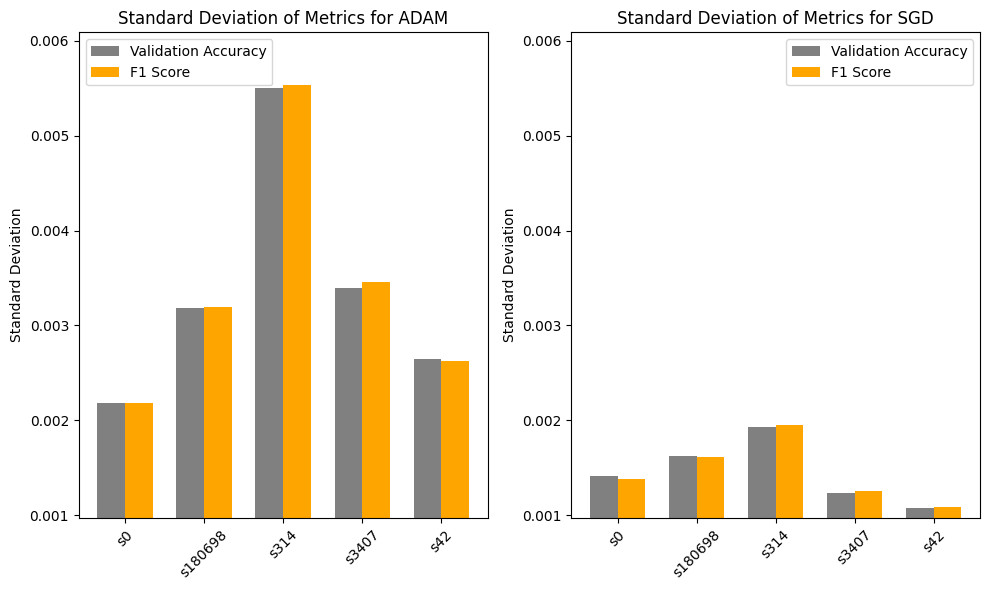
\includegraphics[width=0.8\textwidth]{figures/cifar_std_results.png}
      \caption{Standard Deviation of Performance Metrics for CIFAR-10}
      \label{fig:cifar10_var}
\end{figure}

Referring to Figure \ref{fig:cifar10_var}, the CIFAR-10 task showcases variances in both the F1-Score and Accuracy metrics across two different optimizers. Distinct seed configurations yield varying variance values. A notably higher variance is observed with the ADAM optimizer, suggesting that this optimizer might exhibit greater sensitivity to initial conditions or inherent randomness. The variance values span a range between 0.001 and 0.006, with the peak variance observed for the configuration using seed 314, approximating 0.0055. A close examination of the data also reveals negligible differences in variance between the F1-Score and Accuracy metrics, indicating their congruence in this context.\\


\begin{figure}[h!]
  \centering
  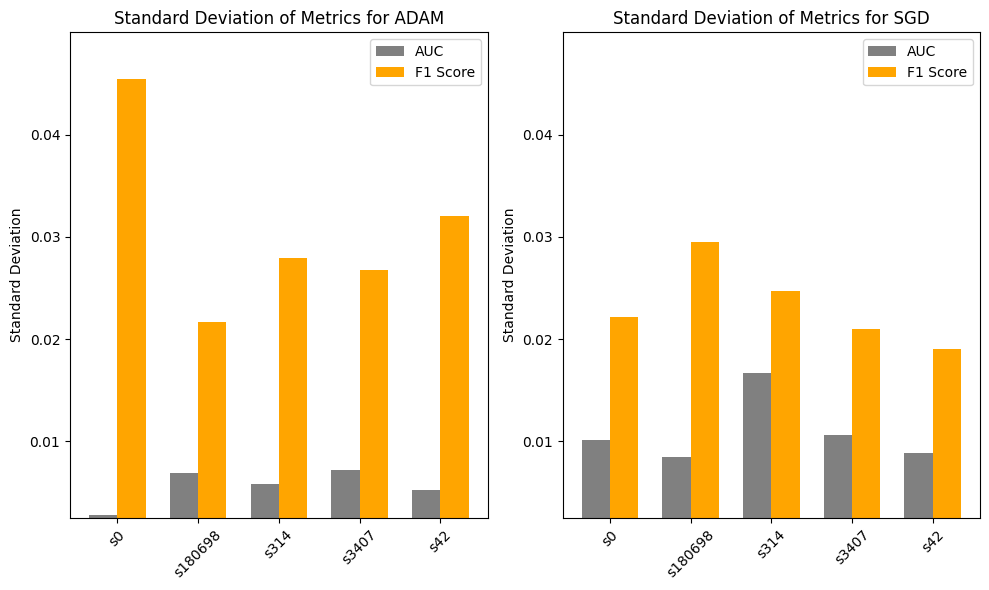
\includegraphics[width=0.8\textwidth]{figures/mammo_results_std.png}
  \caption{Standard Deviation of Performance Metrics for CBIS-DDSM}
  \label{fig:cbisddsm_var}
\end{figure}

Figure \ref{fig:cbisddsm_var} illustrates the standard deviation values for the CBIS-DDSM task. The SGD optimizer exhibits pronounced variances in the AUC score, whereas the ADAM optimizer demonstrates heightened variances in the F1-score. Notably, the overall variance in the F1-score surpasses that of the AUC scores. Moreover the stability of the SGD optimizer against variance appears more consistent, given the relatively minor differences in variances between performance metrics compared to the ADAM optimizer. Moreover, the range of standard deviation values is approximately an order of magnitude greater than observed in the CIFAR-10 task, with the maximum value reaching 0.05 and the minimum at 0.009, particularly evident for the ADAM optimizer with seed 0.\\

\begin{figure}[h!]
  \centering
  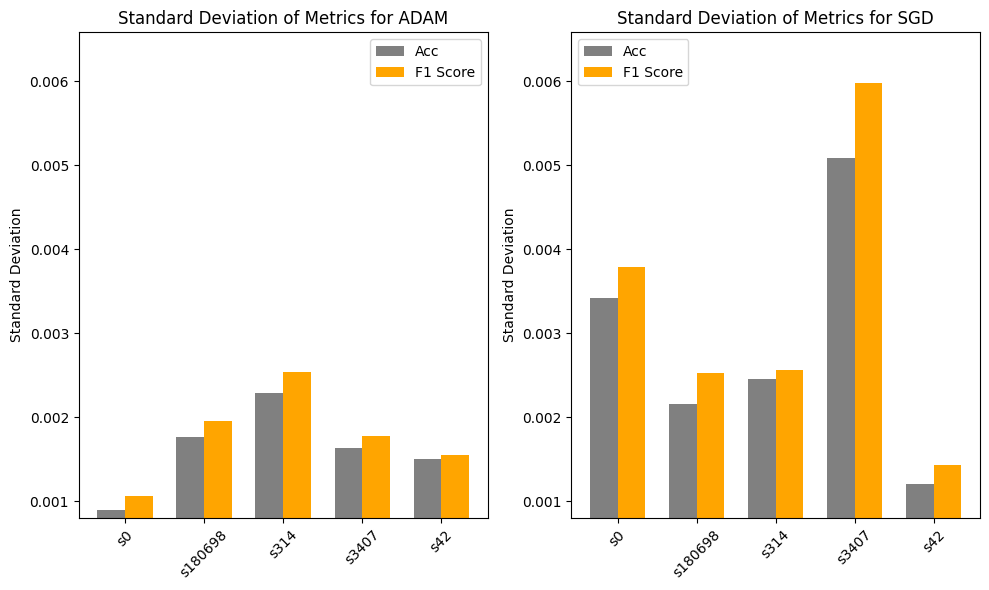
\includegraphics[width=0.8\textwidth]{figures/crack_results_std.png}
  \caption{Standard Deviation of Performance Metrics for SDNET}
  \label{fig:sdnet_var}
\end{figure}

Figure \ref{fig:sdnet_var} presents the variances in performance metrics for the concrete crack detection task. A relatively larger disparity between the F1-score and Accuracy is observed compared to the CIFAR-10 task. Contrary to the previous tasks, the SGD optimizer exhibits higher overall variances for this task. However, the variance range aligns closely with that of the CIFAR-10 task. The apex of variance is identified with seed 3407 using the SGD optimizer.\\

In our analysis of performance variances across tasks, we discerned distinct variability ranges and sensitivities to CUDA-induced randomness. These findings facilitate a deeper understanding of the ramifications of CUDA-related randomness on model performance.\\

\subsection{Runtime and Performance Tradeoff between Deterministic and Non-deterministic Execution}

Since for each seed and optimizer configuration we have one fully deterministic configuration. It would be wise to look at the performances and runtimes to determine the tradeoffs.\\

\begin{figure}[h!]
  \centering
  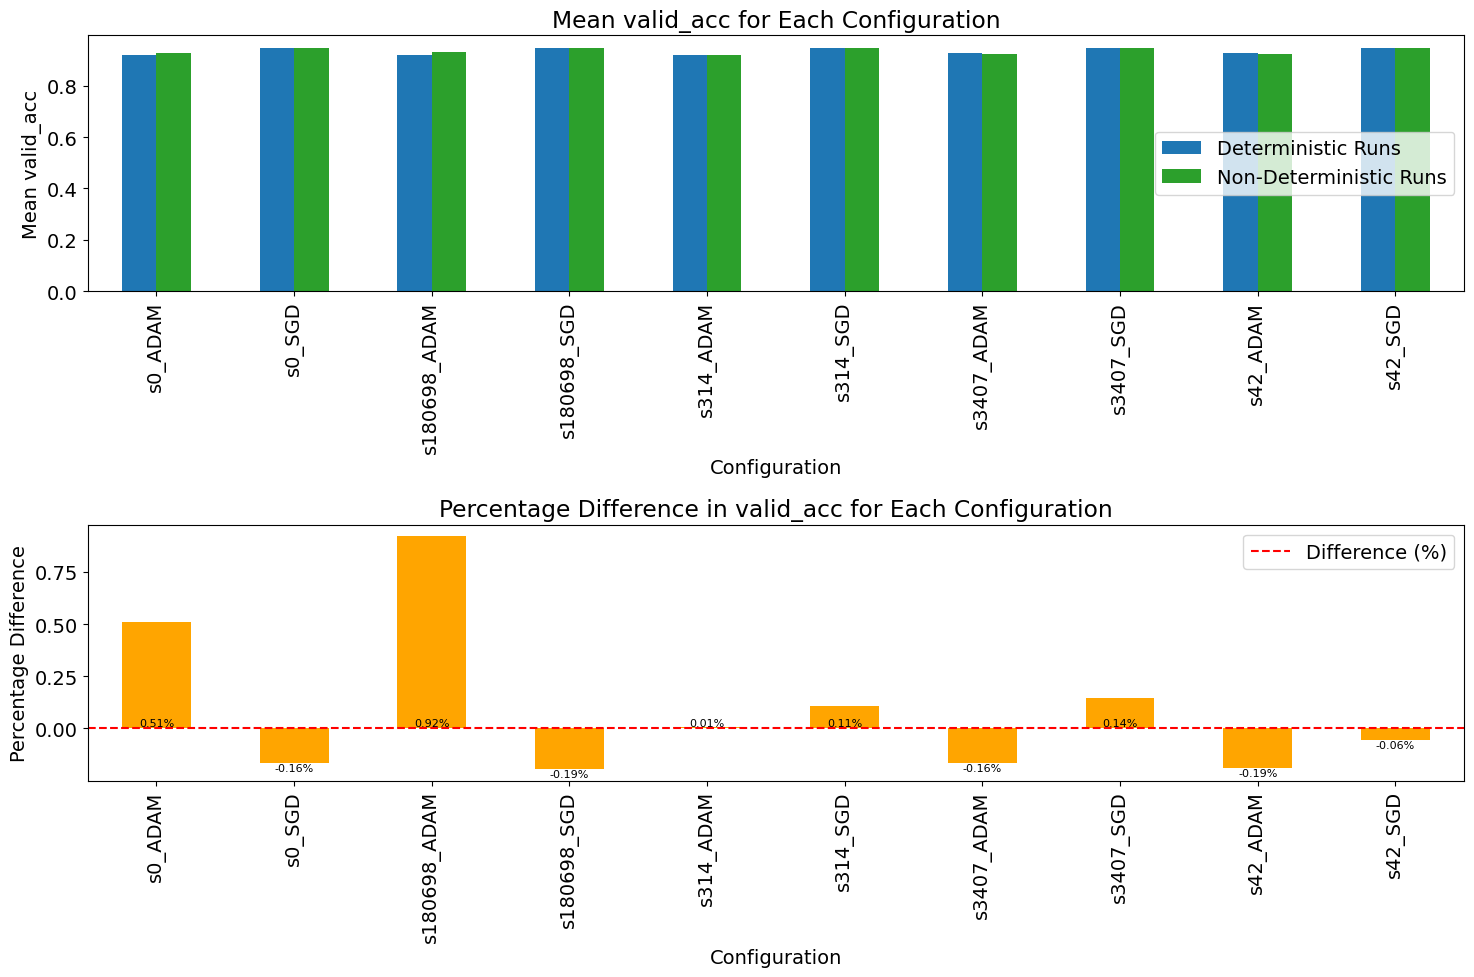
\includegraphics[width=1\textwidth]{figures/cifar_performance.png}
  \caption{CIFAR-10 Differences in Performance between Deterministic and Non-deterministic}
  \label{fig:cifar10_dif_per}
\end{figure}

Above we see the performance difference for CIFAR-10 task, it is clear that at first look there is no jump in performance but on some cases non deterministic execution can benefit from randomness and produce higher results.\\
We observe up to 1\% performance increase in Adam optimizer when using seed value as 180698. From the figures, there is no clear signs that would show that fully deterministic execution increases performance or vice versa.\\

\begin{figure}[h!]
      \centering
      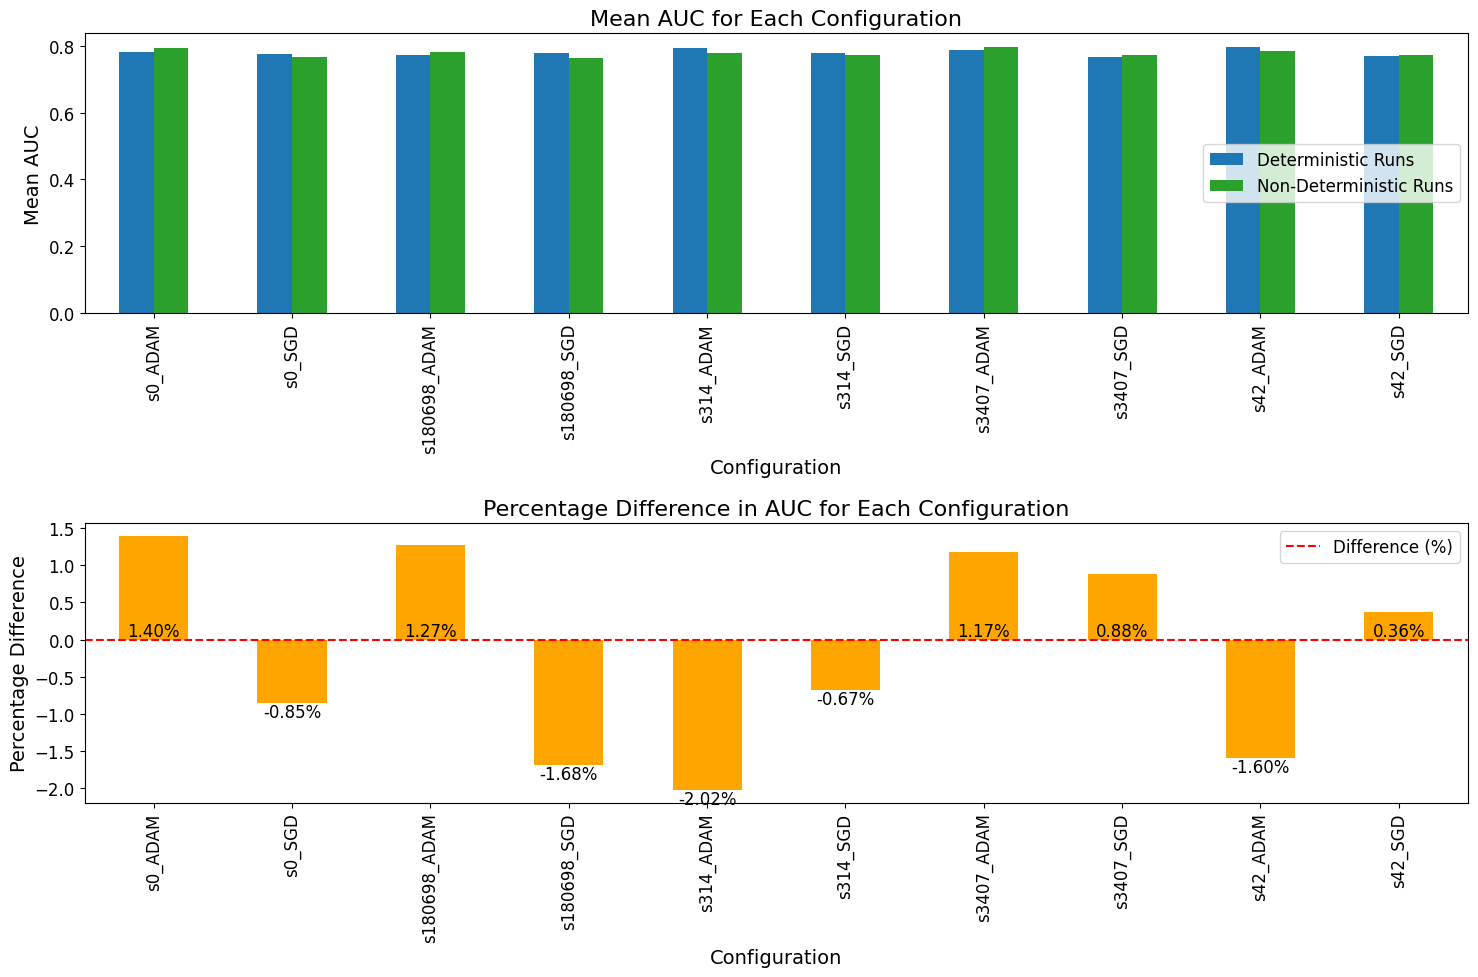
\includegraphics[width=1\textwidth]{figures/mammo_performance.png}
      \caption{CBIS-DDSM Differences in Performance between Deterministic and Non-deterministic}
      \label{fig:cbisddsm_dif_per}
\end{figure}

For the CBIS-DDSM dataset we observe relatively higher differences in AUC scores. There is no clear direction but fully deterministic execution reduced the performance by up to 2 for the seed 314 and increased up to 1.4 for the seed 0.
We observe these extremum values in ADAM optimizer indicating a less stability.\\

\begin{figure}[h!]
      \centering
      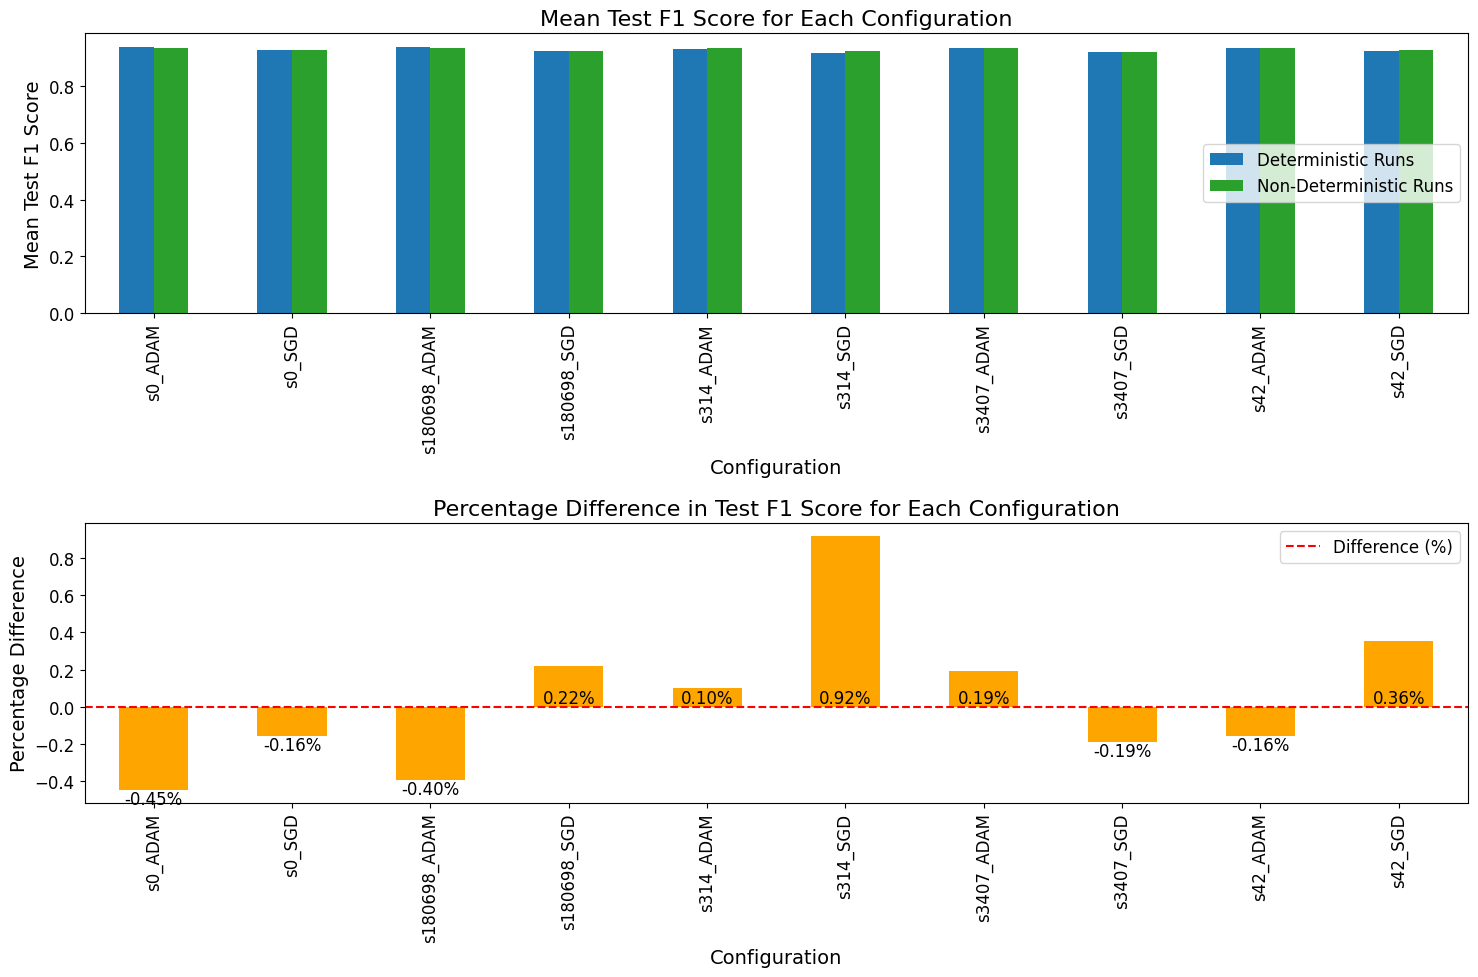
\includegraphics[width=1\textwidth]{figures/crack_performance.png}
      \caption{SDNET Differences in Performance between Deterministic and Non-deterministic}
      \label{fig:sdnet_dif_per}
\end{figure}
In concrete crack detection experiments, like others, we see no visible direction. The range of increase and decrease also similar like CIFAR-10 task. Unlike CIFAR-10, however, highest benefit gained in SGD optimizer with seed as 314. 

\clearpage

\subsection{In Runtime}
\begin{figure}[h!]
      \centering
      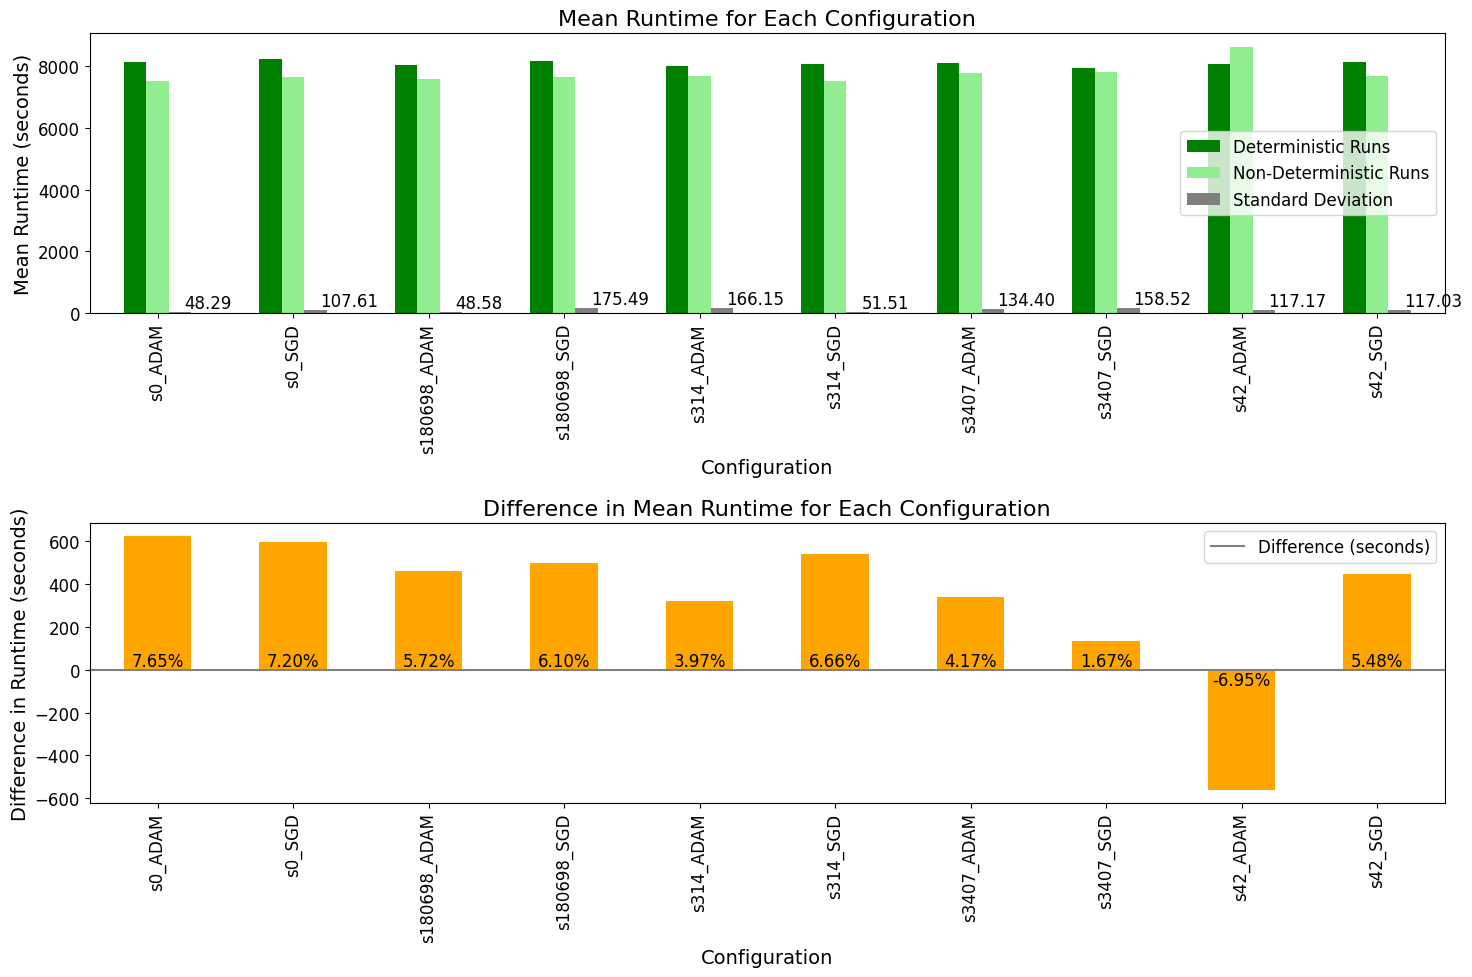
\includegraphics[width=1\textwidth]{figures/cifar_runtime.png}
      \caption[CIFAR-10 Differences in Runtime between Deterministic and Non-\\deterministic]{CIFAR-10 Differences in Runtime between Deterministic and Non-deterministic}
      \label{fig:cifar10_dif_run}
\end{figure}

In runtimes, calculated in seconds, we observe from the figure that deterministic execution takes longer up to 7.65 percent which is in seed value 0 and optimizer as ADAM. 
Note that, longer execution time heavily dependend on the used algorithm change due to deterministic algorithm choices by PyTorch.


\begin{figure}[h!]
    \centering
    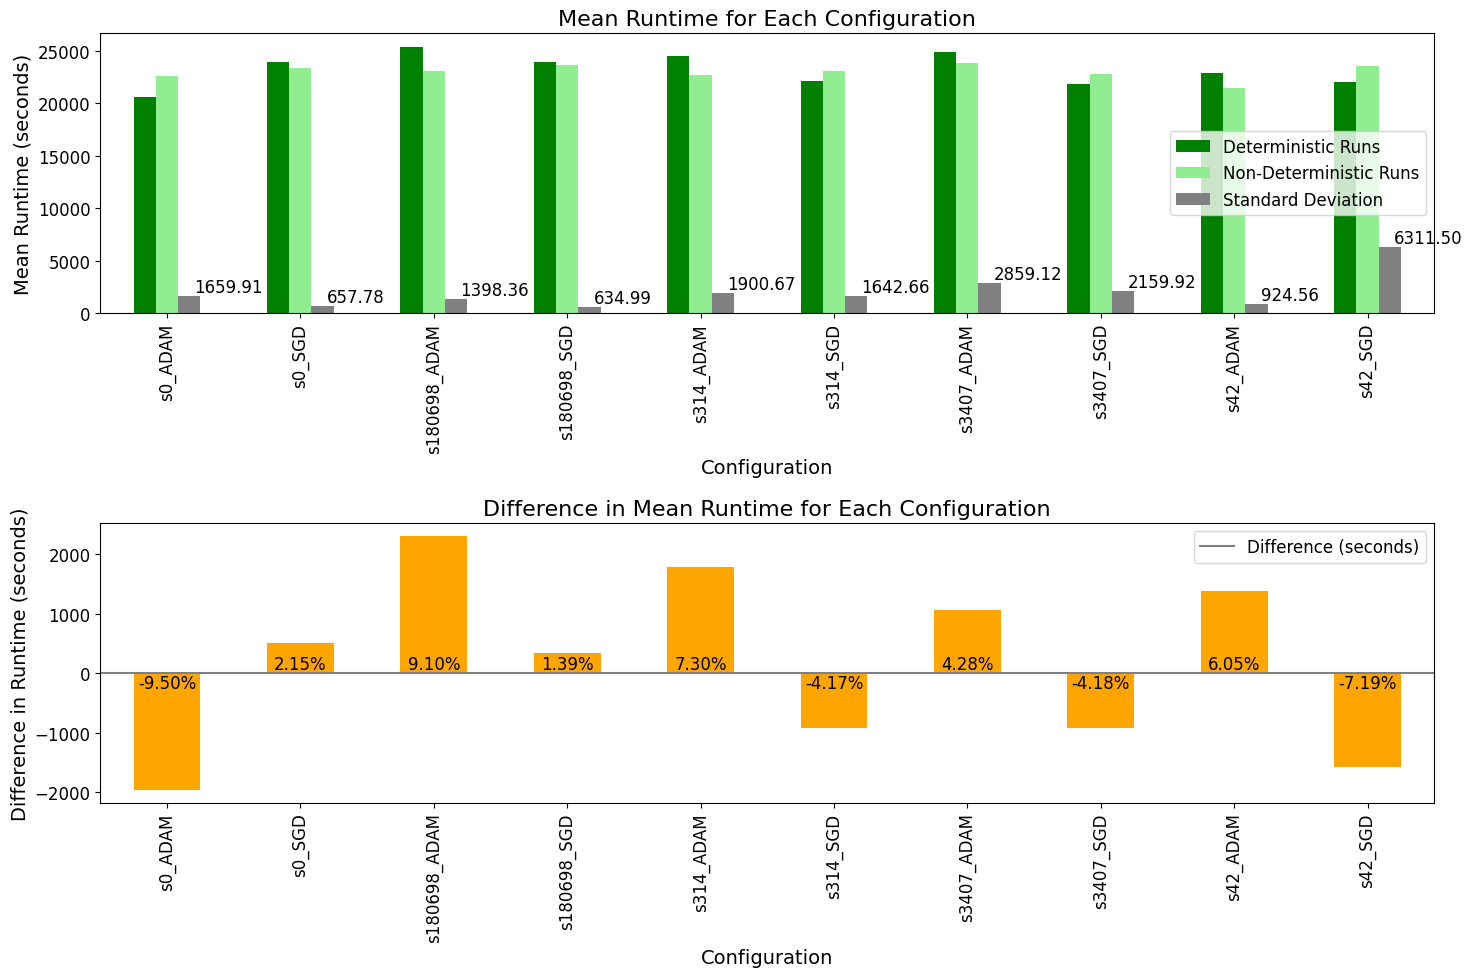
\includegraphics[width=1\textwidth]{figures/mammo_runtime.png}
    \caption{CBIS-DDSM Differences in Runtime between Deterministic and Non-deterministic}
    \label{fig:cbisddsm_dif_run}
\end{figure}

Runtime difference for CBIS-DDSM dataset presented above. Unlike the CIFAR-10, we observe different pattern and no clear direction of runtime tradeoff for the deterministic execution. According the figure, deterministic execution could increase the runtime up to 9 and decrease as well. We observe this extremums in ADAM as seed 0 and ADAM as 180698, respectively. The differences in SGD optimizer are less than the ones in the ADAM. 

\begin{figure}[h!]
    \centering
    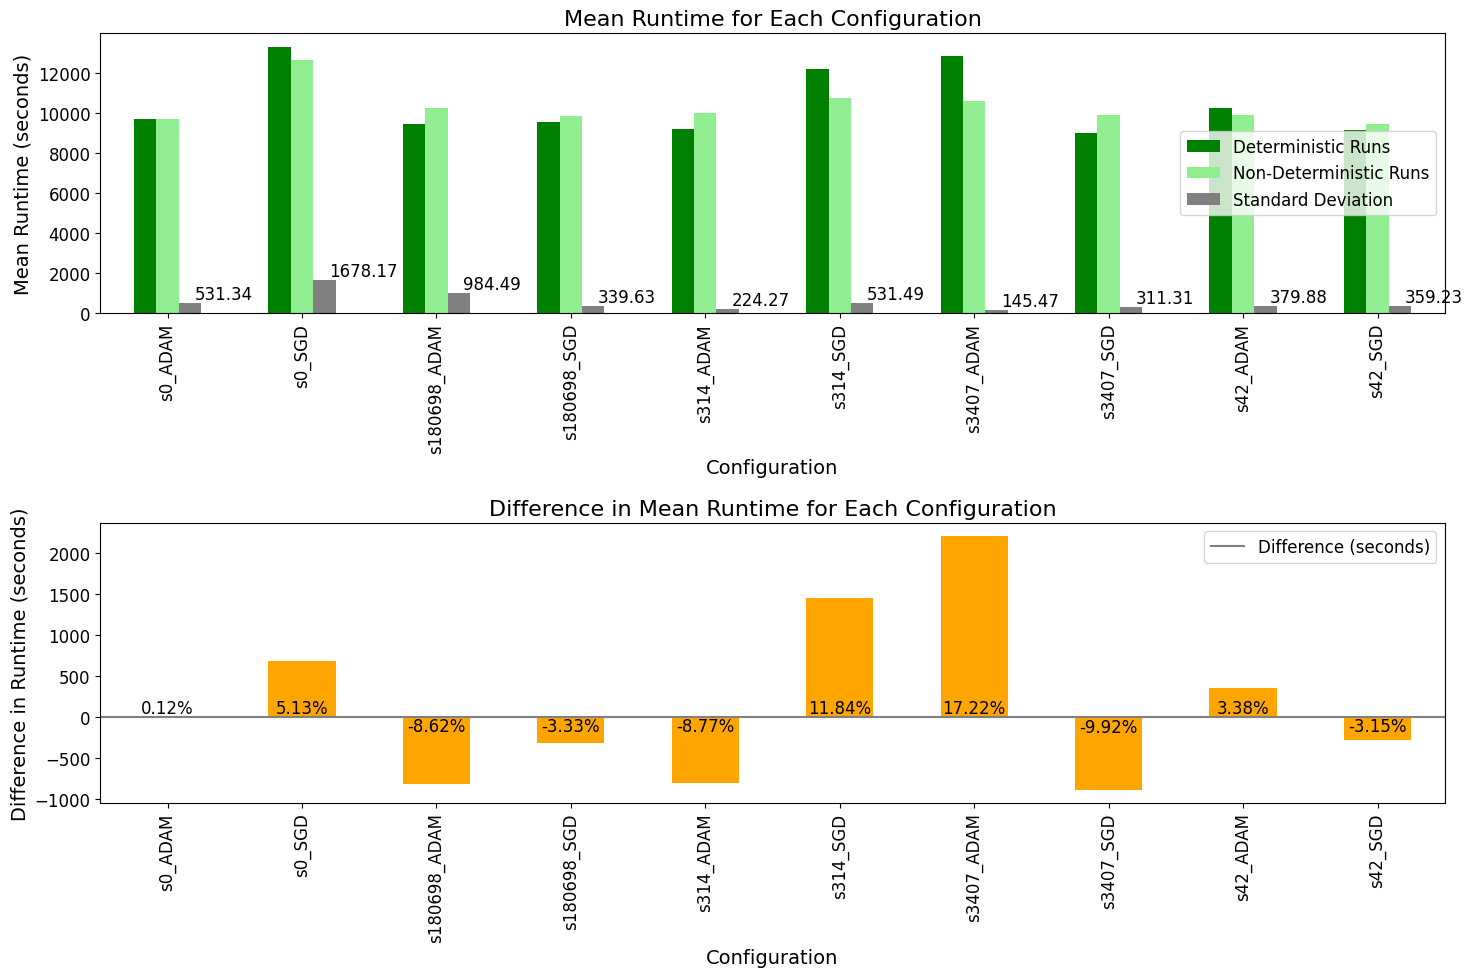
\includegraphics[width=1\textwidth]{figures/crack_runtime.png}
    \caption{SDNET Differences in Runtime between Deterministic and Non-deterministic}
    \label{fig:sdnet_dif_run}
\end{figure}

As for the concrete crack detection, deterministic execution increased the execution time up to 17 in ADAM configuration while second high is 11,84 in SGD. These extremums achieved with seed values as 314 and 3407, respectively.\\

Overall, we observe no clear direction of the runtime impact of the deterministic execution in cases of CBIS-DDSM and SDNET. This is heavily dependent on the used algorithms by the PyTorch framework which we have no direct influence. Also, one can observe from the figures that for each configuration standard variance of the non-deterministic executions are given. If these variances are in the same range then others, this imply that no one particular run one pulled the mean up or down.\\

\section{Weights Analysis} 

On this study,  looking at the performance metrics and runtime can already give lots of idea about the impact and influence the CUDA execution related randomness. However, looking at the weights might give more insight on the matter. Because trained weights are resulted from all mathematical operations and this introduced randomness are directly affecting these operations and ultimately the performances. 
The last layer which is the classification head of the model is what decides the output. We look at the weights on the classification head for this reason. Moreover, the classification head includes all the influence from the previous operations and thus the introduced randomness.\\

On this classification head, depending on the output style we can have a weight matrix of weight vector. By taking all the weights of non-deterministic runs, we can calculate the standart variation component wise and plot this in every checkpoint. With the same logic, we can use some similarity norms and investigate how similar the matrices are.\\

\subsection{Standart deviation of the Weights}

\begin{figure}[h!]
      \centering
      
      % CIFAR-10 Row
      \begin{subfigure}[b]{0.45\textwidth}
        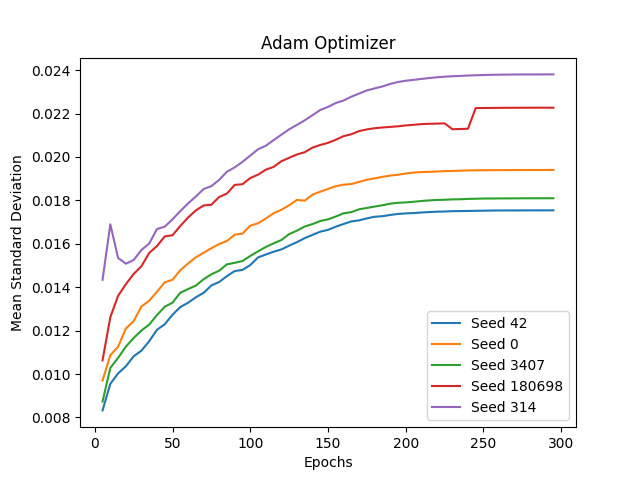
\includegraphics[width=\textwidth]{figures/cifar_adam_curves_std.png}
        \caption{CIFAR-10 Variances for ADAM Optimizer}
        \label{fig:cifar10_adam}
      \end{subfigure}
      \hfill
      \begin{subfigure}[b]{0.45\textwidth}
        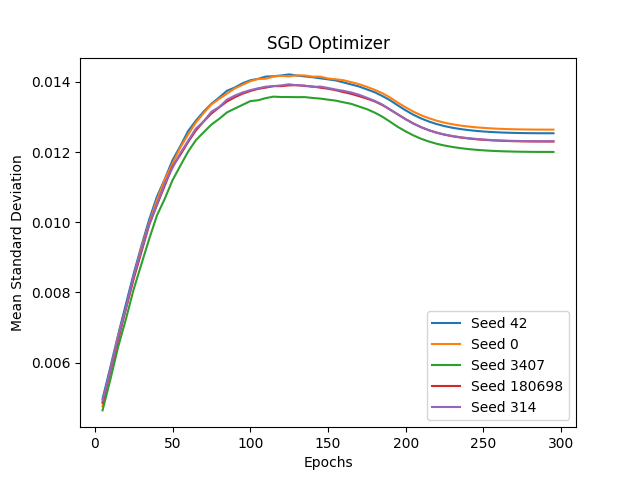
\includegraphics[width=\textwidth]{figures/cifar_sgd_curves_std.png}
        \caption{CIFAR-10 Variances for SGD Optimizer}
        \label{fig:cifar10_sgd}
      \end{subfigure}
      
      % CBIS-DDSM Row
      \begin{subfigure}[b]{0.45\textwidth}
        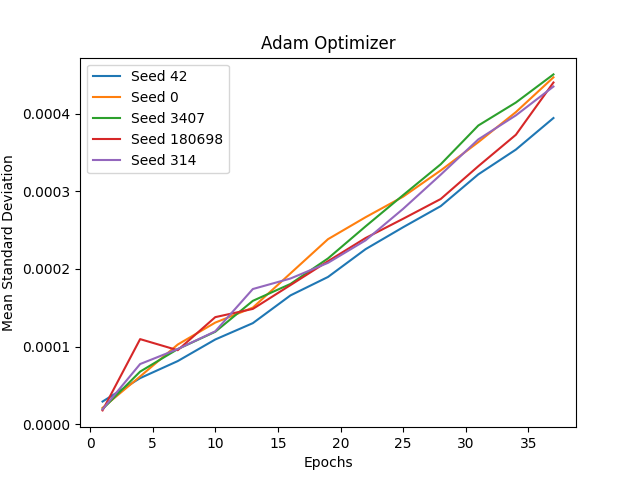
\includegraphics[width=\textwidth]{figures/mammo_adam_curvers_std.png}
        \caption{CBIS-DDSM Variances for ADAM Optimizer}
        \label{fig:cbisddsm_adam}
      \end{subfigure}
      \hfill
      \begin{subfigure}[b]{0.45\textwidth}
        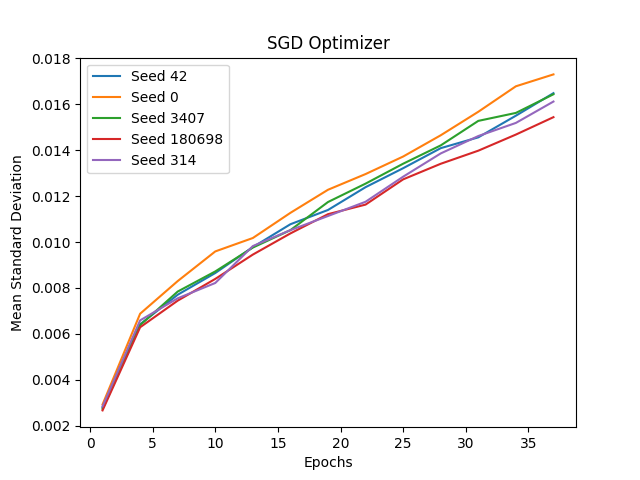
\includegraphics[width=\textwidth]{figures/mammo_sgd_curves_std.png}
        \caption{CBIS-DDSM Variances for SGD Optimizer}
        \label{fig:cbisddsm_sgd}
      \end{subfigure}
      
      % SDNET Row
      \begin{subfigure}[b]{0.45\textwidth}
        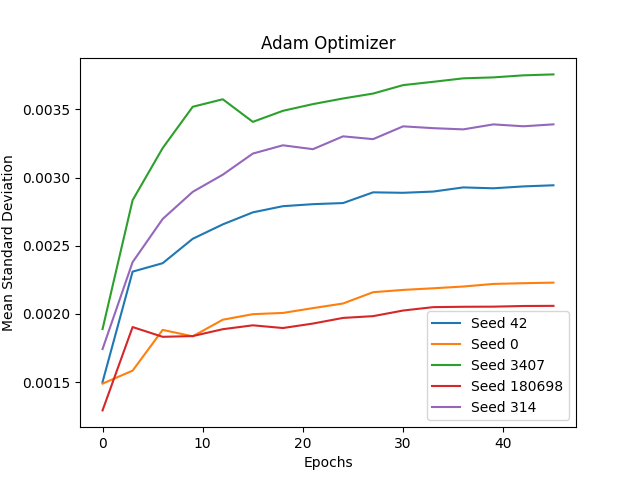
\includegraphics[width=\textwidth]{figures/crack_adam_curves_std.png}
        \caption{SDNET Variances for ADAM Optimizer}
        \label{fig:sdnet_adam}
      \end{subfigure}
      \hfill
      \begin{subfigure}[b]{0.45\textwidth}
        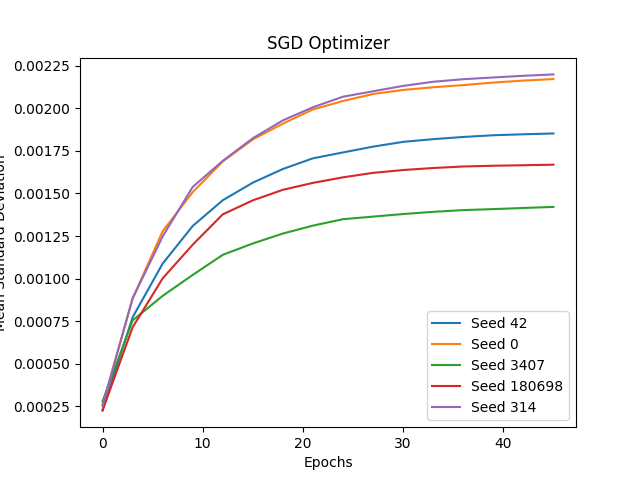
\includegraphics[width=\textwidth]{figures/crack_sgd_curves.png}
        \caption{SDNET Variances for SGD Optimizer}
        \label{fig:sdnet_sgd}
      \end{subfigure}
      
      \caption{Variance plots for different datasets and optimizers}
      \label{fig:variance_plots}
    \end{figure}

\clearpage    
By calculating the standart deviation, we aim to see how diverse is the particular weight index comparing the other identical runs that have inherent cuda randomness.
At a specific epoch, we take the weights from the five non-deterministic matrix and calculate the standart deviation componentwise. We end up with standart deviation matrix with the same dimensions.
Then first we take the mean in first direction then in second direction. As a result for each checkpoints we end up with one value that shows the mean standart variation in that specific epoch.
Below, we present the graphs for the three tasks.\\

In the figure \ref{fig:cifar10_adam}, mean standart deviations accros checkpoints are presentend. We observe
an increasing trend accross epochs. First standart variation values is calculated at fifth epochs so we have already weight updates and thus already far away from the initialization. But the reason that
it increases because we are fixing seed so in first steps weights are actually close to each other then with the CUDA randomness involved with each weight update it gets far away. Whenever the model converges and weights are not updated, we observe constant weights after approximately 200 epochs.
We also observe different seed values resulting in different variances. Seed values 314 and 180698 show less stable trends then the other and we observe some jumps during the training.\\

From the performance metrics we already observed that in CIFAR-10 dataset SGD optimizer shows more stable performance. Figure \ref{fig:cifar10_sgd} also supporst this claim as we see accros seed values similar variances. 
The curves are smoother than the ones with ADAM optimizer as well. Furthermore, unlike ADAM optimizer, with SGD optimizer we achieve decline in variances as the model converges then shows constand trend again.\\
Ultimately, we see lower variances than in the figure \ref{fig:cifar10_adam}\\

In mammography task which results shown in figures \ref{fig:cbisddsm_adam} and \ref{fig:cbisddsm_sgd}, some difficult situations arise and here we only have 40 epochs due to limitations. The model also does not show any concrete improvements after the 40. epoch. However, we see from the figures variances increase during training and we do not know whether they converges or not.
Important point here is that variance values, namely the range of variances are far less then CIFAR-10 dataset. We also see no distinct differences accros different seed values.\\

In the figures \ref{fig:sdnet_adam} and \ref{fig:sdnet_sgd}  we see the mean standart deviations accros epochs for concrete crack detection task for ADAM optimizer.
Unlike other two datasets, seed configurations seems to be more sensitive to the variances. From the start we see upward trend but variances tends to not drastically change after 15.epoch.
We observe the highest variance overall in seed as 3407.\\

For the SGD optimizer, stability seems to be better than the ADAM. Interestingly, we saw in the previous figures related to this task that ADAM optimizer was more stable.
The range of variances and the difference between seed values are also less than ADAM optimizer.
% (fix the labels on the y-axis)\\



\subsection{Similarities}

Apart from the variances, similarities between the weights in the last layer can be calculated. These similarity values can help
identify how much the matrices got far away from each other. Detailed information on how similarities calculated can be found in the previous section.\\

In the below figures that shows these similarities accros datasets and optimizers, we show minimum and mean similarities. While the mean similarities shows us the general trend. 
Minimum similarity indicates the extremum points of two runs that have inherent CUDA execution randomness. We understand from the minimal similarity the maximum potential that this randomness could have.
In the figures, 1 means the matrixes were identical and 0 means their subspace vectors completely orthogonal.
\clearpage

\begin{figure}[h!]
      \centering
      \begin{subfigure}[b]{0.3\textwidth}
        \includegraphics[width=\textwidth]{figures/cifar_similarities_Adam_V2.png}
        \caption{CIFAR-10 Similarities}
        \label{fig:cifar10_adam}
      \end{subfigure}
      \hfill % this will create horizontal space between figures
      \begin{subfigure}[b]{0.3\textwidth}
        \includegraphics[width=\textwidth]{figures/mammo_similarities_Adam_V2.png}
        \caption{CBIS-DDSM Similarities}
        \label{fig:cbisddsm_adam}
      \end{subfigure}
      \hfill
      \begin{subfigure}[b]{0.3\textwidth}
        \includegraphics[width=\textwidth]{figures/crack_similarities_Adam_V2.png}
        \caption{SDNET Similarities}
        \label{fig:sdnet_adam}
      \end{subfigure}
      \caption{Similarities in the Last Layer for ADAM Optimizer}
      \label{fig:similarities_adam}
\end{figure}


Figure \ref{fig:similarities_adam} illustrates the last layer similarities for the ADAM optimizer across various datasets. For the \textbf{CIFAR-10} dataset, the similarities commence at higher values, suggesting that the weights are initially alike. As training advances, these similarities predominantly decrease, indicating a divergence in weights. However, there's a subtle uptrend in the latter epochs, suggesting a resurgence in weight similarity. This trend is more pronounced in CIFAR-10 compared to other datasets. In the \textbf{CBIS-DDSM} dataset, there is a consistent decline in similarity. This consistent reduction may be attributed to the effects of finetuning from ImageNet-initialized weights rather than training from scratch. For the \textbf{SDNET} dataset, a pronounced initial drop is observed, indicating a swift divergence of weights. Yet, the similarities in subsequent epochs decline more gradually, hinting at a plateau in weight divergence. \\

Figure \ref{fig:similarities_sgd} represents the SGD optimizer's performance. The \textbf{CIFAR-10} dataset showcases stability in weight similarities throughout its training. There's a mild upward trend post-convergence, and notably, the weights remain more similar throughout this training phase compared to their ADAM optimizer counterparts. For the \textbf{CBIS-DDSM} dataset, the similarity curve is relatively stable, with a deceleration in the reduction of similarity as training matures. This trend hints at the potential stabilization of weights if training were to be extended. The \textbf{SDNET} dataset, although reminiscent of the ADAM optimizer in trend, is discernibly smoother. As training progresses, the weights tend to maintain their similarity, diverging less than with the ADAM optimizer.\\


\clearpage

\begin{figure}[h!]
      \centering
      \begin{subfigure}[b]{0.3\textwidth}
        \includegraphics[width=\textwidth]{figures/cifar_similarities_SGD_V2.png}
        \caption{CIFAR-10 Similarities}
        \label{fig:cifar10_sgd}
      \end{subfigure}
      \hfill % this will create horizontal space between figures
      \begin{subfigure}[b]{0.3\textwidth}
        \includegraphics[width=\textwidth]{figures/mammo_similarities_SGD_V2.png}
        \caption{CBIS-DDSM Similarities}
        \label{fig:cbisddsm_sgd}
      \end{subfigure}
      \hfill
      \begin{subfigure}[b]{0.3\textwidth}
        \includegraphics[width=\textwidth]{figures/crack_similarities_SGD_V2.png}
        \caption{SDNET Similarities}
        \label{fig:sdnet_sgd}
      \end{subfigure}
      \caption{Similarities in the Last Layer for SGD Optimizer}
      \label{fig:similarities_sgd}
\end{figure}


\clearpage




\section{Statistical Tests} 

Statistical tests are essential tools in research, enabling scientists to infer or deduce properties about a population based on a sample. These tests provide a framework to make decisions or judgments about parameters or datasets by considering the likelihood that an observed outcome would happen due to chance alone.

\subsection{T-Test with Population Mean} 
The t-test is a statistical procedure used to determine whether there is a significant difference between the means of two groups. In this specific application, the t-test is being used to compare the performance values from non-deterministic runs with a known population mean.
The idea behind using the deterministic run as the population mean is grounded in the assumption that the deterministic run will consistently produce the same results regardless of the number of times it is executed. This makes it an appropriate stand-in for the "true" population mean.

Given this setup, the t-test is framed as:

\begin{enumerate}
    \item \textbf{Null Hypothesis ($H_0$)}: There is no significant difference between the performance values of the non-deterministic runs and the deterministic run (population mean).
    \item \textbf{Alternative Hypothesis ($H_1$)}: There is a significant difference between the performance values of the non-deterministic runs and the deterministic run.
\end{enumerate}

The resultant p-value from the t-test signifies the probability of observing the given data (or more extreme data) if the null hypothesis holds true. Conventionally, a threshold of $p < 0.05$ is used to denote statistical significance. A p-value below this threshold implies that the observed data is inconsistent with the null hypothesis, leading to its rejection in favor of the alternative hypothesis.

\begin{table}[h!]
      \centering
      \caption{Statistical Test Results for all datasets}
      \label{tab:stat_results}
      \begin{tabular}{|l|r|l|c|c|c|}
      \toprule
      \textbf{Seed} & \textbf{Optimizer} & \textbf{CIFAR-10 P-Value} & \textbf{CBIS-DDSM P-Value} & \textbf{SDNET P-Value} \\
      \hline
       0 & ADAM & \cellcolor{myred} 0.008406 & \cellcolor{myred} 0.000976 & \cellcolor{myred} 0.000889 \\
      \hline
       0 & SGD & \cellcolor{myyellow} 0.069109 & \cellcolor{mygreen} 0.218819 & \cellcolor{mygreen} 0.429838 \\
      \hline
      180698 & ADAM & \cellcolor{myred} 0.004008 & \cellcolor{myred} 0.033590 & \cellcolor{myred} 0.013022 \\
      \hline
       180698 & SGD & \cellcolor{myyellow} 0.063953 & \cellcolor{myred} 0.026436 & \cellcolor{mygreen} 0.147029 \\
      \hline
       314 & ADAM & \cellcolor{mygreen} 0.975627 & \cellcolor{myred} 0.003490 & \cellcolor{mygreen} 0.463445 \\
      \hline
       314 & SGD & \cellcolor{mygreen} 0.295095 & \cellcolor{mygreen} 0.522252 & \cellcolor{myred} 0.001812 \\
      \hline
       3407 & ADAM & \cellcolor{mygreen} 0.373808 & \cellcolor{myred} 0.046387 & \cellcolor{myyellow} 0.088054 \\
      \hline
       3407 & SGD & \cellcolor{myyellow} 0.069981 & \cellcolor{mygreen} 0.230912 & \cellcolor{mygreen} 0.543679 \\
      \hline
       42 & ADAM & \cellcolor{mygreen} 0.215843 & \cellcolor{myred} 0.005721 & \cellcolor{mygreen} 0.102999 \\
      \hline
       42 & SGD & \cellcolor{mygreen} 0.326455 & \cellcolor{mygreen} 0.516847 & \cellcolor{myred} 0.006795 \\
      \hline
      \end{tabular}
\end{table}


Examining the table, it's evident that different configurations yield varying levels of statistical significance across the datasets. We'll break down the observations dataset by dataset:


\begin{enumerate}
      \item \textbf{CIFAR-10 Dataset}:
      \begin{itemize}
          \item Of the 10 configurations, a mere 2 employing the ADAM optimizer manifest statistically significant results, as evinced by their p-values being beneath 0.05.
          \item A majority of the configurations, notably those using the SGD optimizer, seem congruent with the deterministic run, implying the reliability of results from these configurations.
      \end{itemize}
      
      \item \textbf{CBIS-DDSM Dataset}:
      \begin{itemize}
          \item All configurations that harness the ADAM optimizer have been marked as statistically significant, suggesting potential unreliability of results from these configurations.
          \item A solitary configuration with the SGD optimizer points towards statistical significance.
          \item This insinuates that while the SGD optimizer is predominantly consistent with the deterministic run for this dataset, configurations with the ADAM optimizer might necessitate additional runs or enhanced reproducibility protocols.
      \end{itemize}
      
      \item \textbf{SDNET Dataset}:
      \begin{itemize}
          \item Both the ADAM and SGD optimizers have a pair of configurations each that are flagged as statistically significant.
          \item The remaining configurations seem to be in harmony with the deterministic run, indicating their reliability for the concrete crack detection task.
      \end{itemize}
  \end{enumerate}

In summary, the results highlight the importance of reproducibility and consistency in experiments, especially when working with non-deterministic configurations. The choice of optimizer, as well as other experimental parameters, can significantly influence the reliability of results. It's crucial to consider these factors and conduct appropriate statistical tests to ensure the robustness of findings.

\subsection{ANOVA and Kruskal-Wallis Tests}

In the T-Test with population mean we investigated the the statistical significance for
each configurations. But we can direct our focus on the optimizer sensitivity and use the ANOVA (Analysis of Variance) and Kruskal-Wallis tests. These tests stand out as important tools. Both are designed to determine if there are any statistically significant differences between the means of three or more independent (unrelated) groups. ANOVA, being parametric, is apt for data that is normally distributed. On the other hand, the Kruskal-Wallis test, a non-parametric method, comes into play when the assumption of normality isn't met.\\

For our study's context, these tests offer invaluable insights. They help discern performance differences between various optimizers across multiple datasets. By comparing the means of different configurations for each optimizer, we can determine if an optimizer consistently outperforms others or if the observed differences are mere products of random chance.\\

The results of both tests for the optimizers ADAM and SGD, evaluated across three datasets: Cifar-10, Mammography, and Crack Detection, are presented in Table~\ref{tab:anova_kruskal_results}. The F-Value (for ANOVA) and the test statistic (for Kruskal-Wallis) provide the test's outcome, while the P-Value is our key to determining the significance of these results.\\

\begin{table}[h!]
      \centering
      \caption{ANOVA and Kruskal-Wallis Test Results for Optimizers across Datasets}
      \label{tab:anova_kruskal_results}
      \begin{tabularx}{\textwidth}{
            l
            l
            S[table-format=2.5]@{\hspace{0.65em}}
            S[table-format=1.4]
            S[table-format=2.2]@{\hspace{0.65em}}
            S[table-format=1.4]
            S[table-format=1.2]@{\hspace{0.65em}}
            S[table-format=1.3]
      }
            \toprule
            \multirow{2}{*}{Test} & \multirow{2}{*}{Optimizer} & \multicolumn{2}{c}{Cifar-10} & \multicolumn{2}{c}{Mammography} & \multicolumn{2}{c}{Crack Detection} \\
            \cmidrule(lr){3-4} \cmidrule(lr){5-6} \cmidrule(lr){7-8}
             & & {F-Value} & {P-Value} & {F-Value} & {P-Value} & {F-Value} & {P-Value} \\
            \midrule
            ANOVA          & ADAM & 3.24    & 0.027  &  9.56 & 0.0001 & 2.11 & 0.117 \\
            Kruskal-Wallis & ADAM & 7.73    & 0.101  & 16.78 & 0.0021 & 7.28 & 0.121 \\
            ANOVA          & SGD  & 0.63    & 0.6438 &  0.53 & 0.7086 & 3.43 & 0.026 \\
            Kruskal-Wallis & SGD  & 2.06    & 0.7246 &  2.36 & 0.6693 & 8.66 & 0.069 \\
            \bottomrule
      \end{tabularx}
\end{table}
      
\textbf{ADAM Optimizer:} For the Cifar-10 dataset, the ANOVA test's P-Value stands at 0.027, hinting at significant differences between the means of the groups. However, the Kruskal-Wallis test suggests no significant difference with a P-Value of 0.101. For the Mammography dataset, both tests indicate significant differences between the groups, with P-Values of 0.0001 (ANOVA) and 0.0021 (Kruskal-Wallis). On the Crack Detection dataset, neither test shows a significant difference with P-Values of 0.117 (ANOVA) and 0.121 (Kruskal-Wallis).\\

\textbf{SGD Optimizer:} For the Cifar-10 dataset, both tests converge on the same conclusion: no significant difference in the means of the groups with P-Values of 0.6438 (ANOVA) and 0.7246 (Kruskal-Wallis). Similarly, for the Mammography dataset, both tests indicate no significant difference. However, for the Crack Detection dataset, ANOVA suggests a significant difference with a P-Value of 0.026, while the Kruskal-Wallis test doesn't corroborate this, presenting a P-Value of 0.069.\\

\clearpage




\chapter{Environmental Impact}
\label{chapter:06_enviromental_impact}
% !TeX root = ../main.tex

In scientific research, it is crucial to consider not only the direct results of experiments but also the broader implications and consequences of the research process. While the following environmental assessment is not directly tied to our primary results, it represents an essential facet of our experiments. We believe it is our responsibility to report on the environmental footprint of our work, given the increasing global emphasis on sustainability and the environmental impact of computational practices. Furthermore, we posit that the environmental implications of computational experiments are becoming increasingly significant in the context of sustainable research practices. This perspective aligns with the findings of Ulmer et al.,~\cite{ulmer-etal-2022-experimental}, emphasizing the importance of understanding and reporting the environmental consequences of experimental work.\\

Our experiments were conducted using High-Performance Computing (HPC) resources located in Essen, Germany. The region's electricity generation has a carbon efficiency of \(0.385 \, \text{kgCO}_2\text{eq/kWh}\)~\cite{ourworldindata2023}, with approximately \(43\%\)~\cite{statista2022energy} of the electricity being sourced from fossil fuels. To estimate the carbon footprint of our experiments, we utilized the Machine Learning Impact calculator, as presented by Lacoste et al.,~\cite{DBLP:journals/corr/abs-1910-09700}. This calculator provides a comprehensive framework to quantify the carbon emissions associated with machine learning experiments, considering both the energy consumption of computational resources and the carbon efficiency of the electricity source.

\begin{table}[htbp]
    \centering
    \caption{Energy Consumption and \(\text{CO}_2\) Emission for Different Tasks}
    \label{tab:energy_consumption}
    \begin{tabularx}{\textwidth}{lXXXXX}
        \toprule
        Run Type & Cifar-10 (kWh) & CBIS-DDSM (kWh) & SDNET (kWh) & SUM (kWh) & CO2 (kg) \\
        \midrule
        Experiment runs & 23.42 & 33.02 & 21.25 & 77.69 & 29.91 \\
        All runs & 85.16 & 109.91 & 38.07 & 233.141 & 89.86 \\
        \bottomrule
    \end{tabularx}
  \end{table}
  

From Table \ref{tab:energy_consumption}, it is evident that while the energy consumption and associated carbon emissions for the reported experiments (``Experiment runs'') are significant, the overall environmental impact is considerably higher when accounting for all computational activities, including tests, debugging, and experimental setups (``All runs''). This highlights the broader environmental cost of the entire research process, not just the final reported results. It underscores the importance of energy-efficient algorithms and practices in machine learning research, especially in regions heavily reliant on fossil fuels for electricity generation.


\chapter{Discussion}
\label{chapter:07_discussion}
% !TeX root = ../main.tex
In this chapter, we discuss the implications of our findings, comparing them with existing literature and interpreting their significance in the broader context of safety in AI. The results presented in Chapter 5 provide insights into CUDA-randomness, laying a foundation for further research and potential applications. Additionally, the analysis in Chapter 6 on environmental impact extends the scope of our discussion beyond the technical domain, highlighting the broader implications of our work. As we progress through this discussion, references to visual representations from the preceding chapters will be made to enhance the interpretation and understanding of our results. This discussion aims to provide a deeper understanding of our empirical findings, linking them to the larger narrative of reproducibility and sustainability in AI, and thereby underlining the multi-dimensional significance of this study.\\

In conclusion, we would like to point out that we try to provide some guidelines or suggestions for future research and applications in the field of AI safety. Drawing from our empirical findings and the existing literature, we propose a set of best practices and recommendations that can be adopted by researchers, developers, and policymakers alike. These guidelines not only address the technical challenges identified in our study but also emphasize the ethical and environmental considerations that are crucial for the sustainable development of AI technologies. By integrating these insights into the design, implementation, and evaluation of AI systems, we believe that the AI community can move towards a more responsible and informed approach to innovation. In the subsequent sections, we will delve into these guidelines in detail, providing a roadmap for ensuring that the advancements in AI are both reproducible and sustainable.
\section{Interpretation of Results}

\subsection{Aggregated Results}
In the chapter 5, we presented the results from total 180 runs for each configurations
along with the difference from the mean for all the datasets. We can how the specific configurations
performed on each dataset and how different seeds and optimizers affected the performance of the model and influenced 
by the CUDA-randomness. Apart from the observations made in the chapter 5, we can discuss the 
outcome of the results in the following manner.\\

Table \ref{tab:cifar10_updated} provides an in-depth evaluation of performance metrics on the CIFAR-10 dataset. The SGD optimizer, when initialized with seed 0 in deterministic mode, stands out by achieving an accuracy of 94.96\%. This deterministic behavior implies that the model, under these conditions, consistently predicts the exact same 94.96\% subset of the 10,000 test images across all runs. Conversely, the ADAM optimizer's performance is less consistent. Specifically, when initialized with seed 314 in deterministic mode, it registers the lowest accuracy of 92.17\%. Interestingly, the non-deterministic variant of this configuration trails by a mere 0.01\%. Chapter 5 had previously highlighted the suboptimal performance of the ADAM optimizer on the CIFAR-10 dataset when compared to SGD.\\

The difference from the non-deterministic mean offers further insights. A notable deviation of -0.910\% is observed for the ADAM optimizer with seed 180698, suggesting that its non-deterministic mode has a slight edge, potentially benefiting from inherent randomness. In comparison, the SGD optimizer's maximum deviation is a modest 0.194\%. This data underscores the consistent performance of the SGD optimizer and the relative variability of ADAM, emphasizing the significance of optimizer selection and configuration for achieving optimal results on specific datasets.\\

In Table \ref{tab:sdnet_updated}, the highest accuracy is observed when using the ADAM optimizer with a seed value of 180698 in deterministic mode, achieving an F1-score of 0.9382. In contrast, the lowest score recorded is 0.9158, which is associated with the SGD optimizer and a seed value of 314. Notably, one configuration displayed a significant performance difference, nearly 1\%, between its deterministic and non-deterministic modes. On aggregate, there is an equal number of instances where deterministic configurations outperformed or underperformed their non-deterministic counterparts. However, this variance might be attributed to the inherent benefits of randomness.\\

For the mammography task results presented in Table \ref{tab:cbis-ddsm_updated}, the disparities between deterministic and non-deterministic modes are more pronounced compared to the other two datasets. In the deterministic setting, the ADAM optimizer with a seed value of 42 yielded the second-highest performance, ensuring consistent results. However, the mean performance over five runs with seed 3407 might be lower if additional runs were conducted. The most significant performance gap between the two modes, approximately 2\%, was observed with seed 314 using the ADAM optimizer in deterministic mode with CUDA execution. This difference is deemed substantial within the computer vision community. Intriguingly, the deterministic configuration outperformed the non-deterministic mean by approximately 2\%.\\

Overall, while the aggregated results provide a broad overview of the performance metrics across different configurations, they do not offer granular insights into the nuances of each configuration's behavior. We have presented and briefly discussed these aggregated outcomes to provide an initial understanding. However, it is essential to delve deeper into the trade-offs associated with each configuration, which we will explore in the subsequent subsections. From our preliminary observations, it is evident that individual configurations exhibit optimal performance on specific datasets. Furthermore, the efficacy of the chosen hyperparameters for a given optimizer cannot be understated. Their selection and tuning play a pivotal role in determining the overall performance, a topic we will address in more detail later in this chapter.

\subsection{Variations in Performance}

In this section, we will discuss the variations in performance observed across different configurations. The visualizations are presented for each configuration and for each configuration we reported the two different metrics for the non-deterministic results to test whether different metrics would cause different variability in the performance with CUDA randomness is being free.\\

Starting with the figure \ref{fig:cifar10_var}, the obvious interpretation is that ADAM optimizer introduces 2 to 3 times more variance than the SGD optimizer indicating the less stability in ADAM optimizer in this case. We observe almost zero difference in variance between the two different metric. Additionall, our findings indicate that seed value 314 introduced more variance than others seeds for both optimizer pointing out that regardless of optimizer and hyperparameter selection some specific seeds may produce more variance than others.\\

In the foundational paper~\cite{zhuang2022randomness}, standard variances of 0.001 are observed for the Cifar-10 Dataset when using Resnet18 on an RTX5000. It's noteworthy that they report their results in terms of implementation-level randomness, which primarily encompasses CUDA randomness. In contrast, our study, conducted on an RTX A6000, focuses exclusively on reporting the CUDA randomness. The validity of this comparison is somewhat constrained due to a slight difference in model selection (PreActResnet18). Nevertheless, the best configuration in our study, in terms of standard variances, aligns closely with the results from the base paper. All other variances we observed are higher, with some instances being up to five times greater. At this point, it is important to acknowledge that different seed configuration could yield far more different outcomes so that they can not be ignored when reporting the variability in performance.\\

In Figures \ref{fig:cbisddsm_var} and \ref{fig:sdnet_var}, we present the standard deviation of performance metrics across two distinct metrics. For the CBIS-DDSM dataset, it becomes evident that the F1-score is significantly influenced by randomness. This pronounced variance underscores the relative unreliability of the F1-score for the CBIS-DDSM dataset, especially when juxtaposed with the consistent performance of the AUC score. Additionally, the variance observed across metrics may be attributed, in part, to the choice of optimizer.\\

For the SDNET dataset, a similar trend is observed, with the F1-score exhibiting a marginally higher variance.

In summary, from the three figures presented to elucidate the impact of CUDA-randomness on performance variability across three datasets and two optimizers, we can deduce the following:

\begin{itemize}
    \item The effect of the optimizer is contingent upon the specific dataset in question.
    \item Different performance metrics can manifest varying degrees of variability.
    \item The seed value can also introduce variability in performance metrics.
    \item Notably, the performance variance in the mammography task is markedly greater than that observed in the other two datasets.
\end{itemize}

\subsection{Tradeoffs between Deterministic and Non-deterministic Mode}

In this section, we will discuss the tradeoffs in performance observed across different configurations and provide valuable context for our second research subquestion. We investigate the runtime and performance difference. Before running the experimentations, it is expected that deterministic mode would increase higher runtime than non-deterministic mode ~\cite{zhuang2022randomness}~\cite{pytorch_randomness}. To test this hypothesis, we have plotted the runtime of each configuration in the figures \ref{fig:cifar10_dif_run}, \ref{fig:cbisddsm_dif_run} and \ref{fig:cbisddsm_dif_run}. We also plotted the performance differences in the figures \ref{fig:cifar10_dif_per}, \ref{fig:cbisddsm_dif_per} and \ref{fig:sdnet_dif_per} to see whether the performance difference between deterministic and non-deterministic mode is correlated with the runtime difference or whether there are general performance implications.

\subsubsection*{In Performance}

The performance trade-offs are more discernible in the visual representations compared to the aggregated results presented in Tables \ref{tab:cifar10_updated}, \ref{tab:sdnet_updated}, and \ref{tab:cbis-ddsm_updated}. Beyond the initial discussions, it is evident from the visualizations that certain configurations demonstrate more robust and stable performance than others. Specifically, the SGD optimizer initialized with seeds 42 and 0 exhibits minimal performance disparities between deterministic and non-deterministic modes.\\

Upon examining the three figures, there isn't a consistent trend in the performance differences between deterministic and non-deterministic modes. However, for both the CIFAR10 and crack detection datasets, the performance disparities remain within a 1\% margin. Given this observation, employing deterministic settings may be preferable to ensure reproducibility. In contrast, for the mammography task, the performance differences occasionally surpass the 1\% threshold, with the most pronounced difference being 2\% in favor of deterministic algorithms. It's crucial to note that this particular result is contingent upon a specific seed configuration and may not be universally applicable. Consequently, drawing a generalized conclusion about the performance trade-offs between deterministic and non-deterministic modes remains challenging.\\

\subsubsection*{In Runtime}

One potential limitation of employing fully deterministic settings to ensure complete reproducibility is the associated runtime. An extended runtime could significantly hinder the applicability of deterministic operations in wider contexts. In Figures \ref{fig:cifar10_dif_run}, \ref{fig:cbisddsm_dif_run}, and \ref{fig:sdnet_dif_run}, we illustrate the runtime disparities between deterministic and non-deterministic modes for each configuration. The runtime difference is computed by subtracting the non-deterministic mode's runtime from that of the deterministic mode.\\

For the CIFAR-10 dataset, as depicted in Figure \ref{fig:cifar10_dif_run}, the runtime difference is predominantly positive, suggesting that the deterministic mode incurs a delay of up to 7.65\%. However, this observation is not consistent across all datasets. Specifically, for the mammography dataset, six configurations are slower in deterministic mode, while four are faster. Similarly, for the concrete crack detection dataset, five configurations are slower, and five are faster in deterministic mode. It's crucial to highlight that there is no direct correlation between runtime and performance differences. Additionally, the distribution of slower and faster configurations is such that it leads to a singular observation: deterministic execution does not invariably result in prolonged training times for the mammography and concrete crack detection datasets. Naturally, the algorithms, architectures, and techniques employed play a pivotal role in this, as they influence the algorithmic choices made by PyTorch.\\

\subsection{Weights Analysis}
In previous analyses, we explored the variances and differences in performance, leading to several conclusions. It's recognized in deep learning that the performance of models is significantly influenced by their trained weights. Therefore, examining these weights, especially in the context of inherent CUDA-randomness, can provide a deeper insight into reproducibility and further support our findings.\\

In earlier chapters, we presented the variances and similarities observed in the weights and detailed the methods used for their calculation. In this section, we will discuss the implications of our weight analysis in terms of these variances and similarities. The primary objective is to determine the degree to which the weights are impacted by CUDA-randomness during training.

\subsubsection*{The Standard Deviation in the Weights}

The standard deviation of the weights is illustrated in the set of figures \ref{fig:variance_plots}. Our analysis reveals that the impact of different seed configurations varies across datasets and optimizers. For instance, in the mammography task, the variances with the ADAM optimizer are minimal compared to other variances. However, as observed earlier, the performance variances were notably high. This underscores the challenging nature of the task, where minor fluctuations in weights can significantly affect the model's classification capability. Another observation in this task is the proximity of seed configurations to one another, resulting in negligible differences. A plausible explanation for this could be the pretrained weights. Each model initialization uses the same weights, and fixing the seed predominantly affects other sources of randomness.\\

For the other two tasks, a distinct contrast is evident between the behaviors of the ADAM and SGD optimizers. SGD exhibits greater stability, with variances that are consistently lower than those of the ADAM optimizer. The disparities between seed values are also less pronounced. It's worth noting that, in the concrete crack detection task, the performance variability with ADAM was actually lower than with SGD. However, when examining figures \ref{fig:sdnet_adam} and \ref{fig:sdnet_sgd}, making direct comparisons is challenging since different seeds produce varying variances, and the overall range appears somewhat comparable. Nevertheless, it's unequivocal that the SGD optimizer offers greater stability in weight variances and achieves optimization more consistently. This is particularly evident with the CIFAR-10 dataset, where SGD outperforms in all discussed facets, and the variance further diminishes post-convergence. This suggests that the SGD optimizer is more adept at locating the global optimum compared to the ADAM optimizer.

\subsubsection*{The Similarity of the Weights}

The similarity of each configuration is represented by 30 mini-plots, grouped under two main figures (\ref{fig:similarities_sgd} and \ref{fig:similarities_adam}). Each figure displays the maximum, minimum, and mean similarity values for every epoch. Mirroring our variance analysis, our objective is to ascertain the extent to which the weights are influenced by CUDA-randomness during training. In this context, observing how similarity evolves over the course of training is more insightful than merely focusing on similarity ranges and values. This is because different tasks might exhibit vastly different similarity metrics, making intra-task comparisons more meaningful. It's also crucial to recognize that similarities are profoundly affected by hyperparameter choices. These hyperparameters are selected to optimize accuracy, which means that within a given task, we might encounter either slow or rapid optimization, both of which can significantly shape similarity trends.\\

Bearing these factors in mind, we can deduce that SGD consistently exhibits stable curves, characterized by fewer fluctuations and reduced similarities throughout training. Additionally, the disparity between maximum and minimum similarities in specific configurations is narrower with SGD. Even in the mammography task, we notice a trend towards convergence with potential for further training. In contrast, with the ADAM optimizer, despite the network's convergence, the similarity continues to display a declining trend. While the figures don't conclusively pinpoint which seed configuration offers superior similarity trends, they undeniably highlight the varying influence of different seed configurations on the training process.\\

In a broader context, seed configurations introduce variations in similarity, at times leading to disparities between mean and minimum values or unforeseen shifts in the trends. The choice of optimizer notably impacts this seed-induced sensitivity. Overall, SGD tends to produce more stable and smooth curves and introduces less similarity than ADAM. Furthermore, the selection of the dataset plays a significant role in determining the stability and sensitivity of similarity trends across different seed and optimizer combinations.

\subsection{Statistical Tests}

In our investigation, we analyzed the performance of various configurations, each determined by a unique combination of seed and optimizer. For each such configuration, we executed five runs incorporating randomness and compared these to a deterministic counterpart. Our goal was to ascertain if a specific seed-optimizer combination or more generally one particular optimizer results in performance that significantly diverges from its deterministic behavior or its counterpart.

\subsection*{T-test with Population Mean}

The one-sample t-test, also known as the t-test with population mean, is a statistical procedure employed to determine if a sample of observations could have been generated by a process with a specific mean. In the context of our investigation, we utilize this test to ascertain if the performance of a specific seed-optimizer combination significantly diverges from its deterministic counterpart. To ensure the validity and robustness of this test, it's crucial to understand and satisfy its underlying assumptions.

\begin{itemize}
    \item \textbf{Independence of Observations}: One of the foundational assumptions of the t-test is the independence of observations. In our deep learning experiments, this assumption implies that the outcome of one run of the model should not influence the outcome of another. Given the inherent and uncontrollable randomness introduced by GPU operations, especially the hardware scheduler and floating-point operations, each run's outcome is independent of any other run. This ensures that the results from different runs, even under identical conditions, are not influenced by prior runs.

    \item \textbf{Normality}: The t-test assumes that the differences between the sample means and the population mean are approximately normally distributed. Given the multitude of minute effects influencing each run, such as individual weight initializations, atomic operations, and floating-point arithmetic, the Central Limit Theorem suggests that our results would be approximately normally distributed. However, it's always prudent to conduct preliminary evaluations, such as Q-Q plots, to verify this assumption.

    \item \textbf{Ratio Scale of Measurement}: The accuracies derived from our machine learning models operate on a ratio scale. This means that an accuracy of 0\% signifies the complete absence of correct predictions, and the intervals between accuracy values are consistent and meaningful. As the t-test requires data that supports meaningful mathematical operations and comparisons, our accuracy measurements, being on a ratio scale, fit the requirements of the t-test.
\end{itemize}

It's also important to recognize the distinctiveness of each seed-optimizer combination. In statistical terms, while tests across configurations are independent, they also remain conceptually autonomous. Each combination delineates a separate, individual scenario we aimed to explore.\\

In many statistical analyses, when multiple tests are conducted simultaneously, there arises a concern known as the multiple comparison problem. This problem highlights the increased risk of observing a statistically significant result purely by chance, especially as the number of tests increases. Traditionally, to counteract this risk, corrections like the Bonferroni correction are applied. The Bonferroni method adjusts the significance level based on the number of tests, making the criteria for significance stricter and thereby reducing the chance of false positives.\\

However, given our experimental structure, these traditional concerns associated with the multiple comparison problem don't apply in the typical manner. Unlike many studies where results from different tests are aggregated to claim a single significant outcome or where multiple tests are used to reinforce a singular hypothesis, our approach is distinct. In our investigation, each test is treated as an independent entity, standing on its own merit. Rather than making broad claims, each test specifically addresses a unique question related to its corresponding seed-optimizer pairing. As such, the inherent independence of each test reduces the need for traditional multiple comparison corrections.\\

Furthermore, the practical ramifications of a Type I error (incorrectly rejecting the null hypothesis) in our context are moderate. Each conclusion drawn about a configuration is insulated from the others, ensuring that a potential error in one test doesn't cascade or amplify implications across the entire study.\\

Thus, considering the conceptual independence of tests, the satisfied assumptions, and the isolated implications of potential errors, we argue that the application of the t-test is appropriate for our scenario. Additionally, the Bonferroni correction or similar multiple comparison adjustments would be overly conservative and not scientifically warranted in our particular setup.\\

In the light of these considerations, in the table \ref{tab:stat_results} we present the results of the t-test with population mean for each configuration. 6 p-values out of 10 for the non-deterministic runs that belong the mammography task shows the results are statistically significant indicating that mammography task is heavily influenced by the CUDA-randomness. 
Overall, table indicates a distinct challenges accross different domains indicating the delicate analyses of randomness within the domains and even subdomains. Further analysing the table, we see the huge jumps in the p-values with different seed values. This means that seed value selection might be crucial for the reproducibility of the results and credibility of the findings.\\

\subsection*{ANOVA and Kruskal-Wallis Test}

In the same manner, we also conducted ANOVA and Kruskal-Wallis tests to determine if the performance of a specific optimizer significantly diverges from its counterpart. The same assumptions we made previously could be made in this case as well. The results of these tests are presented in the table \ref{tab:anova_kruskal_results}. We also presented the F-values which is the ratio of the variance between groups to the variance within groups. The F-value is used to determine the p-value which is not presented in the t-test due to space limitations. But the important metric here is the p-value. From the table, we see the p-values with the ADAM optimizer on mammography and CIFAR-10 tasks indicate the statisticaly significant results. Pointing out again that the ADAM optimizer is more
sensitive to the CUDA-randomness than the SGD optimizer. For the concrete crack detection, the p-values with SGD optimizer indicates the statistically significant result but the p-values for ADAM are still close the threshold.\\

\section{Implications of CUDA-Induced Randomness on Reproducibility}
The results of our investigations carry significant implications for the broader deep learning community. Our work aims to illuminate the often-overlooked influence of CUDA-induced randomness on the reproducibility of deep learning experiments. Notably, even in controlled environments, we observed varying sensitivities to CUDA-randomness across different seeds, optimizers, and datasets. Contrary to common belief, our findings indicate that fully deterministic settings don't always compromise performance or increase overhead. In some instances, deterministic configurations outperformed their non-deterministic counterparts, potentially due to the adverse effects of randomness. This phenomenon might be attributed to advancements in hardware, software updates, and sophisticated algorithms and operations introduced by platforms like PyTorch and Nvidia.

To foster a culture of reproducibility and robustness in deep learning research, we offer the following recommendations:

\begin{enumerate}
    \item \textbf{Embrace Deterministic Settings}: Researchers, practitioners, and developers should consider experimenting with fully deterministic settings in their work. The potential benefits, as our findings suggest, could be substantial.
    \item \textbf{Experiment with Multiple Seeds}: To understand the nuances of specific seed configurations, it's crucial to conduct experiments with a variety of seed values.
    \item \textbf{Full Disclosure of Experimental Settings}: For the sake of reproducibility, always report all settings, configurations, and versions used in experiments. This transparency ensures that others can replicate and validate findings.
    \item \textbf{Stay Updated}: With the rapid evolution of hardware and software, it's essential to stay updated. Newer versions might introduce changes that affect reproducibility.
    \item \textbf{Step-by-Step Documentation}: Detailed documentation of every step in the experimental process can significantly aid reproducibility. This includes documenting data preprocessing steps, model architectures, training procedures, and evaluation metrics.
    \item \textbf{Open Source Your Work}: Making your code, datasets, and models available to the public can greatly enhance reproducibility. Open-sourcing not only allows others to replicate your results but also fosters collaboration and accelerates research.
\end{enumerate}

\section{Limitations and Future Work}

Our study, while offering valuable insights into the challenges of reproducibility in deep learning, has certain inherent limitations. Each limitation also presents an opportunity for further research, allowing the community to delve deeper into the nuances of reproducibility and CUDA-induced randomness.

\begin{itemize}
    \item \textbf{Scope of Experiments}: The constraints of this being a master's thesis meant that the number of experiments for each configuration was limited to five. Future research with a more extensive set of runs would provide a more comprehensive understanding and potentially more robust findings.
    
    \item \textbf{Dataset Selection}: The datasets employed in this study were chosen for their representativeness and feasibility. Exploring more extensive datasets like ImageNet, CIFAR-100, or the recently introduced RSNA dataset in future studies might offer different perspectives. The RSNA dataset, as highlighted by Jafari et al.~\cite{jafari2023breast}, shows promise but requires a thorough reproducibility analysis.
    
    \item \textbf{Hyperparameter Selection}: While our hyperparameters were informed by prior studies, a more exhaustive search could be beneficial. The performance of different optimizers can vary based on hyperparameters and can exhibit dataset-specific sensitivities, making this a ripe area for future exploration.
    
    \item \textbf{Related Work on CUDA-Induced Randomness}: The focus of our study on CUDA-induced randomness and reproducibility has shown that there is limited directly-related work in this specific area. This gap indicates a need for further research. Future studies should address the theoretical challenges presented by the CUDA architecture, especially concerning parallel operations and their impact on computation consistency. It might be beneficial to develop mathematical methods to reduce the randomness in computations. Additionally, researching and implementing optimization techniques that have a reduced sensitivity to parallel operations in GPUs could lead to more consistent results in deep learning experiments.
    
    \item \textbf{Architectural Variations}: Different neural network architectures can introduce variability in results. Our study did not explore this potential source of variability, which means different architectures might exhibit distinct sensitivities to CUDA randomness.
    
    \item \textbf{Distributed Settings}: Our non-distributed experimental setup leaves room for investigating the interplay of distributed deep learning with CUDA-randomness, especially as distributed methodologies gain traction.
    
    \item \textbf{Framework-Specific Analysis}: While centered around PyTorch, other frameworks like TensorFlow might have different reproducibility characteristics. A cross-framework analysis, considering the nuances of isolating CUDA-randomness, can offer a broader view of the reproducibility landscape.
\end{itemize}


Our findings shed light on the difficult challenges of ensuring reproducibility in deep learning experiments, emphasizing the subtleties introduced by CUDA randomness. These identified limitations not only highlight areas of improvement for our study but also pave the way for future research directions. We hope this study serves as a catalyst for the research community, underscoring the need for meticulous research methodologies and emphasizing the opportunities that lie in addressing these challenges. The goal is to ensure the robustness and credibility of future deep learning research.


\chapter{Conclusion}
\label{chapter:08_conclusion}
% !TeX root = ../main.tex
% Now, make the conclusions, guidelines and list the main contributions of the thesis.

In the master's thesis, the primary focus was on addressing the reproducibility challenge prevalent in deep learning, with a specific emphasis on computer vision tasks. A unique aspect of the research was the isolation of CUDA randomness, a factor that often introduces variability in deep learning experiments. To provide a comprehensive understanding, a total of 180 training experiments were conducted across three distinct datasets, each representing different domains. The results of these experiments were meticulously analyzed, presented, and discussed to shed light on the complexities of reproducibility in the context of deep learning.\\

We have reached the following key findings:

\begin{enumerate}
    \item \textbf{Achievement of Full Determinism}: By employing fixed seed values, variability is mitigated, constraining randomness. Nevertheless, the randomness introduced by CUDA execution can still influence results significantly. Our experiments demonstrate that with deterministic settings and controlled conditions, complete determinism in deep learning experiments is attainable.
    
    \item \textbf{Determinism vs. Non-determinism Tradeoffs}: Our empirical studies indicate that deterministic execution introduces minimal computational overhead, making its adoption practically advantageous. However, in certain scenarios, a performance decline of up to 2\% was noted, which is significant for specific applications. The decision to employ full determinism should be based on the specific requirements and anticipated outcomes of the model.
    
    \item \textbf{Domain Specificity}: The influence of randomness during training varies with the dataset's domain. Specifically, the Breast Cancer Dataset exhibited a pronounced effect of randomness, underscoring the reproducibility challenges in medical imaging.
    
    \item \textbf{Role of Optimizers}: Different optimizers display distinct stability levels when confronted with randomness from CUDA execution. Notably, the ADAM optimizer showed reduced stability, indicating heightened sensitivity to such randomness.
    
    \item \textbf{Analysis of Model Weights}: While performance metric variations are insightful, they might not offer a holistic view of the randomness in the training. Analyzing the model's trained weights can yield deeper insights into the randomness's effect on training.
    
    \item \textbf{Metric Sensitivity}: The metrics' susceptibility to randomness might depend on the dataset's domain. For instance, in the breast cancer study, the F1-score was more vulnerable to randomness compared to the AUC score. Therefore, when selecting and reporting evaluation metrics, the metrics' sensitivity to randomness should be considered.
\end{enumerate}


\appendix
\chapter{Appendix}
% What kind of info can go here? Related to used materials, tools, and frameworks? 
% and some additional info that might not be related to results directly but details to the interested readers and to reproduce the results ?
% TODO: add more chapters here

\appendix{}

\printbibliography{}

\end{document}
